% ---- ETD Document Class and Useful Packages ---- %
\documentclass{ucetd}
\usepackage{subfigure,epsfig,amsfonts}
\usepackage{natbib}
\usepackage{amsmath}
\usepackage{amssymb}
\usepackage{amsthm}
% Add extra packages I need
% Packages used by pandoc when converting Markdown to LaTeX
\usepackage{longtable}
\usepackage{booktabs}
\usepackage{tabularx}
% Make cross-references hyperlinks (also format URLs with \url).
% Specify breaklinks so that titles in table of contents linewrap.
\usepackage[breaklinks]{hyperref}
% Fix to use hyperref with UCETD template (from Jason Torres)
\renewcommand{\etdChapterHeadFormat}[1]{\uppercase{#1}}
% Ability to split long captions across pages
\usepackage{ccaption}
% Crop figures
\usepackage{graphicx}
% Add footnote to List of Tables about the supplementary files
\renewcommand{\listtablename}{List of Tables
  \footnote{Note: Due to the large size of some tables, the tables
  have been provided in a supplementary file accompanying the
  dissertation. In such cases, the page number provided below directs
  the reader to a table's caption.
}}
% Nice tilde
% http://tex.stackexchange.com/questions/9363/how-does-one-insert-a-backslash-or-a-tilde-into-latex/9372#comment47661_9372
\newcommand{\mytilde}{\raise.17ex\hbox{$\scriptstyle\mathtt{‌​\sim}$}}
% Add packages to make list with multiple letters
% https://tex.stackexchange.com/questions/12279/outline-of-style-i-a-i-a-1
\usepackage{outlines}
\usepackage{enumitem}
\setenumerate[1]{label=\Roman*.}
\setenumerate[2]{label=\alph*.}
\setenumerate[3]{label=\roman*.}
\setenumerate[4]{label=\Alph*.}
% try rotating table
\usepackage{rotating}
\usepackage{graphicx}
% use tabulary for wrapping text in tables
\usepackage{tabulary}
% math short hyphen
\mathchardef\mhyphen="2D
% get accents in bibliography
\usepackage[utf8]{inputenc}
\usepackage[T1,T2A]{fontenc}
% declare alpha as
\DeclareUnicodeCharacter{3B1}{$\alpha$}

%% Use these commands to set biographic information for the title page:
\title{Investigating molecular mechanisms and dynamics of Ena/VASP and other actin binding proteins}
\author{Alyssa Justine Harker}
\department{Biochemistry and Molecular Biophysics}
\division{Biological Sciences}
\degree{Doctor of Philosophy}
\date{December 2018}

%% Use these commands to set a dedication and epigraph text
\dedication{Dedication Text}
\epigraph{Epigraph Text}

\begin{document}
%% Basic setup commands
% If you don't want a title page comment out the next line and uncomment the line after it:
\maketitle
%\omittitle

% These lines can be commented out to disable the copyright/dedication/epigraph pages
\makecopyright
%\makededication
%\makeepigraph


%% Make the various tables of contents
\tableofcontents
\listoffigures
\listoftables

% Enter Acknowledgements here
\acknowledgments
I am very thankful for all the support and assistance I've received during my PhD. None of these projects would have been possible without the work from my collaborators. In addition to my main project, I was able to add to many other people's projects  and, while doing so, learned many new topics and different techniques which I greatly appreciate. 

I was very fortunate to be able to work in such a great environment as the Kovar Lab. I would like to thank past and present members of the Kovar Lab, specifically Katie Homa, Alisha Morganthaler, Caitlin Anderson, Jenna Christensen, Glen Hocky, Patrick McCall, Dennis Zimmermann, Tom Burke, Kate Proudfoot, and Meghan O'Connell for their scientific insights and making the Kovar Lab a fun, collaborative, and productive place to do science. Furthermore, I would like to thank Jon Winkelman and Cristian Suarez for their training and guidance, especially when I first joined the lab. I would finally like to acknowledge my advisor David Kovar for his guidance and support throughout my entire graduate school career as well as the freedom to explore.

I would like to thank my committee Bob Keenan, Margaret Gardel, and Mike Rust for taking the time to meet with me and give me advice about my project. I appreciate the different persepectives and ideas that they brought during our meetings over the course of my PhD. I would also like to thank the administrators that make the cluster and departments run smoothly, specifically the administrators I worked closely with, Kristine Gaston and Lisa Anderson. 

I have also benefited from being part of the larger molecular biosciences community. I appreciate the support my molecular biosciences cohort has given me from when we started this journey during coursework and rotations through the stresses and celebrations that occur throughout graduate school. I would like to thank those who gave me scientific advice and insights, but specifically Ashley Rich and Ana Beiriger who also supported my hobbies and allowed me to maintain balance during graduate school. I would also like to thank my BMB year Katherine Leon, Chris Katanski, and Phil McGilvray who are an outstanding source of encouragement and laughter. Furthermore, Within the BMB community as a whole, I could rely on sharing of advice, reagents, and knowledge.

My friends and family have given me unending support through my time at University of Chicago. I would specifically like to thank my parents, Mark and Amy Harker, and my sister, Emily Harker, for their limitless encouragement and willingness to assist in any way. I would finally like to thank Corey Rodriguez who supports me in everything I do and is a constant source of motivation and encouragement.

% Enter Abstract here
\abstract
Many important cellular functions depend on the architecture of a dynamic actin cytoskeleton forming at the correct location and time during the cell cycle. Cellular division, motility, and endocytosis are a few examples of processes in which actin filaments must be nucleated, polymerized, severed, and depolymerized at the precise time and location in the cell.To create a complete picture of the dynamic actin cytoskeleton, it is vital to collect mechanistic information about diverse actin networks and their associated proteins. Actin networks gain their distinct properties from the subset of hundreds of actin binding proteins that localize to them. Some of these actin binding proteins, such as formin, have molecular mechanisms of how the singluar protein interacts with actin that are well-studied. However, how these proteins interact with other actin binding proteins and how this affect's their mechanisms and leads to complex actin networks is only just being appreciated. Nonetheless, it is important that we first discerned the molecular mechanism of these proteins on their own as this gives us a base mechanism to guide further experimentation. Understanding the mechanistic details of actin binding proteins allows us to determine how they can function collectively to create, maintain, and disassemble complex actin networks. 

Here I investigate the molecular mechanisms of various actin binding proteins and how they are affected by the presence of other actin binding proteins and actin-binding toxins. The main project focuses on Ena/VASP, which are tetrameric actin elongation factors that bind F-actin barbed ends continuously while increasing their elongation rate within dynamic bundled networks such as filopodia. However, we were also interested in how Ena/VASP's molecular mechanism is affected by the presence of different bundling proteins. We used single-molecule TIRFM and developed a kinetic model to dissect Ena/VASP’s processive mechanism on bundled filaments. The results demonstrate that Ena tetramers are tailored for enhanced processivity on fascin bundles and avidity of multiple arms associating with multiple filaments is critical for this process. 

I also was involved in many collaborations to investigate the dynamics and molecular mechanisms of various actin binding proteins. Many of these projects also surround the bundling proteins that I had studied in relation to Ena/VASP. I found that fascin, which is the main bundling proteins in filopodia and also an enhancer of Ena/VASP run lengths, also plays a role in reducing Arp2/3 complex-mediated branching. We also showed that fascin sorts with $\alpha$-actinin due to an intrinsic sorting mechanism dictated by filament spacing. We visualized this sorting by electon microscopy and observed the transition between a fascin domain and an $\alpha$-actinin domain. Further invesitgation into $\alpha$-actinin's bundling properties showed that tropomyosin increases $\alpha$-acintin dynamics. My other collaborations were focused on the pathogenic \textit{Vibrio} bacteria. We found that an excreted toxin formed actin oliogomers that inhibited Ena/VASP elongation and caused Ena/VASP to cap filaments. Furthermore, we investigated the molecular mechanism of a \textit{Vibrio} nucleation factor VopL/F and found that they nucleate filaments from the pointed end of F-actin and stay bound at the pointed end before releasing the filament. 

Overall, my work has shown the importance of not only characterizing the molecular mechanism of actin binding proteins, but also how these actin binding proteins work in concert with the multiple other actin proteins that are found within the cell. The gained knowledge from these studies are a step forward for the field to fully grasp the role each actin binding protein plays in the larger system of the actin cytoskeleton. 


\mainmatter
% Main body of text follows

% Chapter 01 - Introduction
% Chapter 01
% Insert figures: Ena/VASP and formin from review, bundler summary, cell depicting networks, actin filament and monomer structure?, TIRF

\chapter{Introduction}\label{ch:intro}
As the most abundant protein in most eukaryotic cells, actin participates in more protein-protein interactions than any known protein \citep{dominguez_actin_2011}. All eukaryotes have have at least one gene for actin and many have complex actin networks with only a single actin gene, such as budding yeast, fission yeast, and green algae \citep{pollard_actin_2016}. However, some species have many actin genes that are expressed in different tissues. For example, Humans have three genes for $\alpha$-actin, one gene for $\beta$-actin, and two genes for $\gamma$-actin and plants can have 10 or more actin genes \citep{pollard_actin_2016}. Additionally actin is highly conserved among organisms and, even among the three isoforms ($\alpha, \beta, \gamma$-actin) in vertebrates, only varies by a few amino acids near the N-terminus \citep{dominguez_actin_2011}. The actin cytoskeleton plays many biochemical and mechanical roles in the cell and is important for many cellular processes such as polarity establishment, motility, and morphogenesis \citep{blanchoin_actin_2014}. To fulfill these roles, the actin cytoskeleton forms distinct and dynamic networks made up of filamentous actin (F-actin) and other actin binding proteins (ABPs). These networks are formed and degraded at certain times and locations within cells for proper cellular function. 

\section{Actin}\label{actin-intro}

Actin is a 46 kDa globular protein and contains four subdomains. The N-terminus is located in subdomain 1, then the polypeptide domain proceeds through subdomains 2, 3, and 4, returning to subdomain 1 with the C-terminus \citep{pollard_actin_2016}. Subdomains 1 and 3 are structurally similar though contain little sequence similarity \citep{dominguez_actin_2009,pollard_actin_2016}. Subdomains 1 and 2 form the outer domain while 3 and 4 form the inner, larger domain. Between these domains is a hinge region and two large clefts, a nucleotide binding cleft and a target binding cleft. The nucleotide binding  cleft binds ATP and an associated cation (Mg\textsubscript{2+} in cells). Many proteins bind actin in the target-binding cleft between subdomains 1 and 3 \citep{dominguez_actin_2009}.

Actin assembles into polar filaments with new subunits being primarily added onto the barbed end (subdomains 1 and 3) versus the pointed end (subdomains 2 and 4). The polarity of the filaments was initially observed when visualizing actin filaments saturated with myosin heads using electron microscopy \citep{huxley_electron_1963}. The myosin heads formed an arrowhead-shaped object and thus defined the "barbed" and "pointed" end of the filament due to which direction the arrowheads were pointing. An actin filament contains two protofilaments that wrap around each other with a right-handed twist along the long-axis \citep{hanson_structure_1963}. However, the repeated unit of symmetry is a left-handed helix with \mytilde13 actin subunits repeating every 35.9 nm. The G-actin to F-actin transition consists of a 12-13$^\circ$ rotation of the outer domain (subunits 1 and 2) with respect to the inner domain (subunits 3 and 4) with some additional bending movements of subdomains 2 and 4. Therefore, F-actin is flatter than F-actin and the D-loop in subdomain 2 inserts into the target-binding cleft of the subunit above \citep{dominguez_actin_2011}.

Actin monomers bind both ATP or ADP tightly and a nucleotide-free G-actin will rapidly acquire ATP with a Kd in the nanomolar range \citep{de_la_cruz_nucleotide-free_1995}. A bound nucleotide stabilizes an actin monomer, but is not required for polymerization \citep{pollard_actin_2016}. Monomers polymerize spontaneously under physiological salt conditions with cations present. This spontaneous assembly has an initial lag period due to the slow nucleation step caused by the instability of actin dimers and trimers \citep{cooper_kinetic_1983, frieden_polymerization_1983, sept_thermodynamics_2001}. Once the fourth subunit has been added to the actin nucleus, the seed is more stable and elongation occurs at the same rate as longer filaments. Barbed ends elongate 10 times faster than pointed ends. ATP-actin associates with barbed ends with a rate constant of \mytilde10 $\mu$M\textsubscript{-1} s\textsuperscript{-1} and slowly dissociates at \mytilde 1 s\textsuperscript{-1} \citep{pollard_rate_1986}. Thus the 'critical concentration' for monomer addition is 0.1 $\mu$M for the barbed end of actin filaments. Once a monomer undergoes the conformational change to bind to a filament, the rate of hydrolysis increases to 0.3 s\textsuperscript{-1}. Hydrolysis is thought to occur randomly along the filament \citep{jeno_internal_1995}, though it has been proposed that neighboring subunits could effect the rate \citep{korn_actin_1987}. Once hydrolysis occurs, the phosphate is slow to dissociate \citep{carlier_direct_1986}, leaving ADP-actin which dissociates more easily from both ends. 

The total cellular concentration of actin is between 50-200 $\mu$M. In cells, filaments assemble and disassemble on the timescale of tens of seconds. Actin binding proteins (ABPs) cause large differences from the \textit{in vitro} rates and allow for almost half of the total actin in cells to be unpolymerized (\mytilde25-100 $\mu$M) which is far above the critical concentration. Within cells there is millimolar concentrations of Mg-ATP and phosphate, so most cytoplasmic G-actin has bound Mg-ATP. Once the G-actin is added to F-actin, the Mg-ATP is hydrolyzed and then the phosphate is released. Depolymerization of F-actin releases Mg-ADP monomers, where ADP is exchanged for ATP. The ADP to ATP exchange is slow, but can be sped up by an actin monomer binding protein, profilin \citep{pollard_actin_2016}. The rates are further changed by ABPs that nucleate, elongate, cap, sever, and crosslink filaments. 

\section{Actin networks}\label{network-intro}
The actin filaments in cells are organized into distinct, dynamic networks that allow the cell to carry out processes such as cytokinesis, endocytosis, motility, and adherence. A set of ABPs localize to each distinct network, which allows for each network's unique architecture and function. One simplified model organism, S. Pombe fission yeast, only has one actin isoform, yet has three distinct actin networks: actin patches for endocytosis, actin rings for cytokinesis, and actin cables for polarity establishment. Here I will focus on three actin networks found in higher eukaryotes; lamellipodia, filopodia, and stress fibers. 

\subsection{Lamellipodia}\label{lamellipodia-intro}
The lamellipodium is made of short, branched actin filaments that form a thin, dense meshwork \citep{small_lamellipodium:_2002}. Lamellipodia can extend up to tens of microns along the leading edge of motile cells \citep{skau_specification_2015}. The branched network is nucleated by the Arp2/3 complex, which must be activated by a nucleation promoting factor (NPF) such as WAVE or WASP proteins \citep{blanchoin_actin_2014}. The branches are kept short by capping protein, which blocks barbed end filament growth and filaments are severed for recycling by cofilin. The growth of the dense network pushes on the leading edge membrane generating force. Lamellipodia polymerization drives the membrane forward when membrane tension is low, but drives cell movement when membrane tension is high and the cell is adhered to a surface through retrograde flow \citep{skau_specification_2015}.  

\subsection{Filopodia}\label{filopodia-intro}
The dynamic fingerlike projections that emerge from the lamellipodium are called filopodia. Filopodia are important for exploration of the mechanical and chemical extracellular space of motile cells \citep{mattila_filopodia:_2008}. This is especially important in steering neuronal growth cones, wound healing, and dorsal or ventral closure during development. During these processes cells must be able to follow mechanical and chemical signals in order to move through space towards other cells or locations \citep{bornschlogl_how_2013}. Filopodia are made up of 10-30 tightly packed filaments, primarily bundled by crosslinking protein, fascin \citep{vignjevic_role_2006, mellor_role_2010}. These filaments form parallel bundles, with all their barbed ends organized towards the tip of the filopodia \citep{bornschlogl_how_2013}.

There are two proposed models for how filopodia form at the leading edge of cells: convergent elongation \citep{yang_filopodia_2011} and de-novo nucleation \citep{faix_filopodia:_2009}. The convergent elongation model proposes that the filaments for filopodia are initially nucleated by Arp2/3 complex in the lamellipodia. These filaments make $\lambda$-shaped precursors that can then be bundled by fascin \citep{svitkina_mechanism_2003,small_lamellipodium:_2002}. In contrast, the de-novo nucleation proposes that filopodia formation is distinct from the lamellipodium and nucleation of these filaments is facilitated by formins such as mDia2 \citep{faix_making_2006,mellor_role_2010}. It could be that different nucleators are driving different types of filopodia in different cell types. Futhermore, some cells can produce different types of filopodia within the same cell. For example, S2 cells from \textit{Drosophila} have short, more dynamic filopodia formed by Ena compared to formin Dia \citep{bilancia_enabled_2014}. This is also seen in mammalian cells where VASP or mDia2 expression facilitates varying number of filopodia with different dynamics and morphology \citep{barzik_ena/vasp_2014}. 

\subsection{Stress Fibers}\label{stressfibers-intro}
Another way that cells can produce force through actin networks is contractile stress fibers. Stress fibers are formed from actinmyosin bundles formed mainly by $\alpha$-actinin. There are three main types of stress fibers in animal cells: ventral, dorsal, and transverse arcs. Ventral stress fibers are anchored at each end by focal adhesions where dorsal stress fibers are only anchored at one end near the leading edge. Transverse arcs are convex stress fibers that form parallel to the leading edge \citep{burridge_focal_2016}. Stess fibers and focal adhesions are important for cell adhesion, morphogenesis, and especially mechanotransduction \citep{tojkander_actin_2012}. Stress fibers are the main vehicle for contractile forces in cells. The contractile force is formed by myosin II that binds alternating with $\alpha$-actinin along the stress fibers \citep{naumanen_mechanisms_2008}. 

\section{Actin binding proteins}\label{abps} 
Actin binding proteins (ABPs) can nucleate, elongate, cap, sever, disassemble, and crosslink F-actin. ABPs also can bind to actin monomers, such as profilin. Profilin is a small actin binding protein that has high affinity for ATP-actin monomers (Kd = 0.1 $\mu$M) \citep{pollard_actin_2016}. However, profilin binds monomers on the barbed end so it inhibits nucleation and elongation at the pointed end, though allows elongation at barbed ends. When a profilin-actin complex binds the barbed end, the conformational change in the actin subunit decreases profilin's affinity facilitating dissociation. Profilin is also important for catalyzing nucleotide exchange in actin monomers \citep{mockrin_acanthamoeba_1980, vinson_interactions_1998}. Between profilin and another actin monomer binding protein, thymosin-$\beta$4, there is a low concentration of free actin monomers \citep{pollard_actin_2016}.

Other ABPs can bind to sides of F-actin, such as tropomyosin and myosin. Tropomyosin is a coiled-coil protein that binds along the long-pitch helices of F-actin \citep{ecken_structure_2015}. Tropomyosin stabilizes filaments and increases its persistence length \citep{sousa_electron_2010}. Additionally, in muscle cells tropomyosin regulates the binding of myosin. Myosin is a family of ATP-motors that bind and release actin filaments throughout the ATP hydrolysis cycle. Depending on the type of myosin, this allows processive runs along actin filaments or muscle contraction in sarcomeres. Myosins are important for force generation, transport of cargo along F-actin, anchoring organelles, and mechanotransduction \citep{hartman_myosin_2012}.

\subsection{Nucleation factors}\label{nucleators}
As described earlier, actin nucleation is slow; therefore, in cells ABPs catalyze the formation of an F-actin seed. There are three different classes of these nucleation factors. The first class is the Arp2/3 complex. The Arp2/3 complex is made up of seven subunits including Arp2 and Arp3, which are actin related proteins (Arp). Arp2/3 complex nucleates filaments by binding to the side of a mother filament and using its Arp2 and Arp3 proteins to template the nucleation of a filament that branches from the mother at a 70$^{\circ}$ angle. Arp2/3 nucleates filaments for the lamellipodia, some stress fibers and actin patches in S. pombe \citep{pollard_actin_2016,naumanen_mechanisms_2008,mishra_yeast_2014}. Arp2/3 is inhibited by profilin. MORE here or later? Arp2/3 is activated via WAVE or WASP.

The second class of nucleation factors are formins, which nucleate unbranched filaments. There are still some open questions surrounding how formins nucleate filaments \textit{in vivo}. Initially, it was thought that formins could stabilize actin dimers with their FH2 domain to aid in nucleation, since the FH2 domain is necessary and sufficient for nucleation \textit{in vitro} \citep{zigmond_formin-induced_2004,paul_role_2008,pring_mechanism_2002}. However, it was found that FH2 domains are inefficient at nucleating profilin-actin, which is thought to be the main substrate available \textit{in vivo}. Recently it has been shown that C-terminal tail regions of certain formins, FH1 domains, and NPF that bind to the C-terminal tail region could assist the FH2 domain for profilin-actin nucleation \citep{breitsprecher_formins_2013}. Formins can nucleate filaments for the lamellipodia, filopodia, some stress fibers, and contractile rings \citep{faix_filopodia:_2009,mishra_yeast_2014,blanchoin_actin_2014}.

The third class of nucleation factors are WH2 nucleators. This is a much broader class than the other two and contains proteins such as Spire, Cobl, and bacterial VopL and VopF (VopL/F) \citep{quinlan_drosophila_2005, namgoong_mechanism_2011, burke_bacterial_2017,siton-mendelson_functional_2017}. This is a more recently discovered class of nucleators that use tandem WH2 domains to bind and bring together actin monomers to form a nucleus. The proteins in this class have variable nucleation activities, caused by the differences in the number of WH2 domains and also the length of linkers between them \citep{siton-mendelson_functional_2017}. As an example, VopL/F are virulence factors from bacteria \textit{Vibrio parahaemolyticus} and \textit{Vibrio cholera} that can assemble unproductive F-actin in host cells \citep{liverman_arp2/3-independent_2007}. VopL/F contains three tandem WH2 domains and dimerizes through a VopL/F C-terminal domain (VCD). However, two different mechanisms were proposed for VopL and VopF, two closely related proteins. One mechanism suggested that VopL nucleates actin filaments from the pointed end \citep{namgoong_mechanism_2011,yu_mechanism_2011,zahm_bacterial_2013}, while the other mechanism proposed that VopF nucleated filaments then continued to assemble actin at the barbed end, similar to a formin \citep{pernier_dimeric_2013}.

\subsection{Elongation factors}\label{elongators}
Beyond nucleation, there are also assembly factors that aid in actin elongation. Actin will assemble spontaneously at a rate of \mytilde10 $\mu$M s\textsuperscript{-1} \citep{pollard_rate_1986}; however, there are ABPs that associate with the growing barbed end and can change this polymerization rate. Formins are able to increase the elongation rate of F-actin using profilin-actin \citep{pollard_actin_2016}. Another elongation factor protein is Enabled/Vasodilator stimulating phosphoprotein (Ena/VASP). These tetrameric proteins use WH2-like domains to associate with the barbed end and can increase F-actin elongation with both actin and profilin-actin. I will return to these two proteins to look closer into their mechanisms and functions.

\subsection{Bundling proteins}\label{bundlers}
(figure here)
There are different families of proteins that are able to crosslink F-actin. These proteins contain more than one actin binding domain so that they can bind to more than one filament at a time. Crosslinking defined as holding two filaments together at one point. In contrast, bundling is when two filaments are held parallel to each other by multiple crosslinks \citep{pollard_actin_2016}. I will use bundling protein to describe proteins that are able to bundle filaments \textit{in vitro}, though their main function in cells may be to crosslink rather bundle filaments. 

The largest group of bundling proteins fall in the CH domain superfamily, such as fimbrin/plastin, $\alpha$-actinin, spectrin, and filamin. These proteins use two sets of tandem CH domains to bind to two actin filaments. Fimbrin contains two tandem CH domains to bundle F-actin as a monomer and localizes to the lamellipodia and base of filopodia in cells. Fimbrin bundles have narrow spacing, \mytilde10-12 nm, and can consist of antiparallel and parallel filaments \citep{hanein_atomic_1998}. Alpha-actinin also uses CH-domains to bundle actin but only contains one tandem CH domain per monomer so to bundle F-actin it must form a dimer using its spectrin repeats. $\alpha$-actinin bundles have much wider spaced filaments and can also contain either parallel or antiparallel filaments \citep{sjoblom_alpha-actinin_2008}. Different $\alpha$-actinins have slightly different spacing due to the number of spectrin repeats that separate the CH domains. For example, \textit{S. Pombe} Ain1 contains just two spectrin repeats compared to human $\alpha$-actinin IV, which contains four \citep{murphy_actinin_2015}. $\alpha$-actinin and fimbrin bind on the same site of the actin filament \citep{klein_2004}. In contrast, fascin bundles F-actin using its four $\beta$-trefoil domains \citep{jansen_mechanism_2011}. Fascin is a small globular bundling protein that is the main bundling protein in filopodia \citep{vignjevic_role_2006,mellor_role_2010}. Fascin forms bundles that are narrowly spaced, between 8-10 nm, and only consist of parallel filaments \citep{edwards_fascins_1995,jansen_mechanism_2011,cant_drosophila_1994}. 

\section[Ena/VASP and Formins]{Ena/VASP and Formins\footnotemark}\label{ena-formin-review}

\footnotetext{Portions of this section were modified from a review in preparation with Jonathan Winkelman.} 

\subsection{Comparison of processive actin elongation factors}

Mechanistic understanding of the actin cytoskeleton and ABPs is important for understanding how each protein works individually, but also how the different proteins effect each other and contribute to proper function of cellular processes. I am interested in looking at the molecular mechanism of ABPs to understand how proteins are properly functioning, but also how with different diseases and mutations the proteins fail to function. This detailed mechanistic understanding is the foundation that cell biology can be built upon, leading to deeper knowledge of processes that occur in cells and even organisms. 

Here I will focus on the mechanism of two processive protein families, formins and Ena/VASP, which bind to the barbed end of actin filaments and affect actin filament polymerization. Interestingly, though these two families have different structures and use distinct mechanisms, they share similarities in how they increase actin polymerization as well as that they are both localized to the leading edge and involved in filopodia formation. However, their mechanistic differences in terms of processive run lengths, diverse protein binding partners, and formin's reliance on profilin actin bring up many interesting questions concerning how these proteins are utilized by a cell within different and even the same processes. The knowledge of formin's mechanism is a step ahead of Ena/VASP's, exploring the role of force, rotation, and diverse actin regulatory domains on its actin assembly properties. However, this allows insight to compare and contrast the two processive machines and understand how they both individually and concurrently help to assemble the necessary actin networks for proper cellular function. 

\subsection{Cellular processes}\label{ena-formin-cellular-processes}

\subsubsection{Ena/VASP}

Ena/VASP processes: actin polymerization
Bundling and nucleation in vitro, not sure in vivo implications, cell migration?
Vasodilator-stimulated phosphoprotein (VASP) was first discovered in human platelets as a substrate of both the cAMP- and cGMP-dependent protein kinases \citep{halbrugge_analysis_1990}. Simultaneously, enabled (ena) was found in Drosophila during a genetic screen for surpressors of abelson protein tyrosine kinase mutant phenotypes \citep{gertler_genetic_1990}. Ena and VASP were found to be homologous \citep{ahern-djamali_identification_1999} and homologs have been found in all multicellular metazoan cells and Dictyostelium \citep{sebe-pedros_insights_2013}.
Invertebrates (Drosophila, C.elegans, Dictyostelium ect.) only have one isoform of Ena/VASP while mammalians have three: Mena (mammalian Enabled), VASP, and EVL (Ena-Vasp-like) \cite{gertler_mena_1996}.
Ena/VASP localization: lamellipodia, filopodia, stress fibers, and focal adhesions adherence junctions

\subsubsection{Formin}

Formin homology proteins (formins) are highly conserved actin binding proteins that function in multiple cellular processes such as cytokinesis, oogenesis, and stress fiber and filopodia formation. Furthermore, formins can interact with both actin and microtubules \citep{bartolini_formin_2008,henty-ridilla_accelerated_2016}, allowing for communication between these two cytoskeleton systems. Formins were first discovered as mutations at the mouse limb deformity (ld) locus resulting in development defects \citep{woychik_formins:_1990}. Since their discovery the formin family has grown, now counting 15 different formins in mammalian cells. The formins are localized to different areas of the cell including the leading edge, tips of filopodia, cell-cell junctions, and cytokinetic rings. As a class, formins are implicated in nucleation of nascent actin filaments, processive elongation, and competition with capping protein as well as other F-actin barbed end binding proteins. However, there are some proteins within the formin family (i.e. INF2) that have been shown to carry out additional behaviors, such as depolymerization, bundling of filaments, severing, or actin monomer binding \citep{gurel_assembly_2015}. Though the mechanism of formin-mediated processive filament assembly has been well-studied, the individual characteristics of different formins and how those characteristics influence their distinct roles within the same cell continue to be open questions. 

\subsection{Domain organization}\label{ena-formin-domains}

\subsubsection{Ena/VASP}
N-terminal Ena-VASP homology 1 (EVH1) domain: localization, FP4 binding (FPPPP) such as formin, zyxin, lamellipodin, vinculin \citep{ball_dual_2000,niebuhr_novel_1997,klostermann_orthologous_2000}.
EVH1 present in all Ena/VASP family members as well as distantly related Wiskott-Aldrich syndrome proteins, WASP and N-WASP, and Homer/Vesl family, though proteins from outside the Ena/VASP family recognize different domains. Structurally the EVH1 domain is similar to pleckstrin homology (PH) and phosphotyrosine-binding (PTB) domains though there is little sequence similarity to these domains \citep{prehoda_structure_1999,reinhard_actin-based_2001,ball_dual_2000} [fedorov structure.
The C-terminal Ena/VASP Homology 2 (EVH2) domain contains the main actin binding domains. The G-actin binding domain (GAB) is related to a WH2 domain which also binds actin monomers. The F-actin binding domain (FAB) and the C-terminal coiled-coil facilitates tetramerization. Interestingly, it was found that mammalian proteins can form heterotetramers in vitro \citep{riquelme_selectivity_2015}. 
Between the EVH1 and EVH2 domain is a poly-proline region. This region can bind to profilin and other SH3 containing molecules such as Abl, Src \citep{lanier_abl_2000,gertler_mena_1996}.

\subsubsection{Formin}
The classical formin homology 1 (FH1) and formin homology 2 (FH2) domains are the characteristic  domains of the formin family. The N-terminus of formin contains regulatory and localization domains that vary depending on the subfamily of formins. The largest subfamily, Diaphanous-related formins (DRF), is autoregulated by the N-terminal Diaphanous inhibitory domain (DID) binding to a C-terminal Diaphanous autoregulatory domain (DAD).  Rho-GTPase binding to the N-terminal GTPase binding domain (GBD) can relieve this autoregulation. Subsets outside of DRFs have C-terminal DAD or Wiskott-Aldrich syndrome homology region 2 (WH2) domains. Other domains are found across the diverse formin family, including those that function in auto-regulation, inhibition, localization, depolymerization, and filament actin (F-actin) binding.

The FH1 and FH2 domains have canonically been associated with the formins' actin assembly properties and dimerization. The FH1 domain contains between one to 15 polyproline repeats that are able to bind to profilin, but with varying affinity. This domain is flexible and allows for increased actin filament elongation in the presence of profilin-actin likely by increasing the local concentration of actin monomers near the polymerizing barbed end (ref). The FH2 domain forms a head-to-tail dimer that is thought to stabilize an actin dimer, promoting nucleation of a nascent actin filament. The dimerized FH2 domains can additionally encircle and remain associated with the barbed end of an actin filament, facilitating the addition of profilin-actin to the barbed end during elongation. For a detailed review of the FH1 and FH2 domains, see \citep{paul_review_2009}. 

\subsection{Mechanism of processive F-actin elongation}\label{ena-formin mechanism}

\subsubsection{Ena/VASP}
G-actin or profilin-actin transfered to barbed end. Change in conformation of G-actin once it adds to the filament allows for release of newly added monomer. 
Doesn't fall off like formins with a certain number of steps. Actin concentration independent \citep{hansen_vasp_2010}.
Rotation not known
All arms equal?
Clustering in vivo?

\subsubsection{Formin}

There are two main models for formin processive elongation, stair stepping and stepping second. Both models incorporate an over-rotation of the short-pitch helical twist at the barbed end from native F-actin state of $167^{\circ}$ to $180^{\circ}$ when FH2 is tightly bound. FH2 exists in a dynamic equilibrium between the tightly bound “closed” state ($180^{\circ}$) and loosely bound “open” state ($167^{\circ}$). The closed state does not allow addition of new monomer because the filament is over rotated and does not present favorable contacts for an incoming subunit \citep{otomo_structural_2005}. The initial model, stair stepping, describes the FH2 bound tightly to three actin subunits in the closed state. The FH2 domain can then transition to an open state by releasing one actin binding contact. This allows a monomer to bind to the barbed end and FH2. With the addition of a new monomer, the FH2 can return back to the closed state. Therefore, the FH2 domain translocates first, then facilitates monomer addition \citep{otomo_structural_2005}. 

The stepping second model reverses these steps and proposes that monomer addition promotes a translocation. Importantly, the translocation state is the most loosely bound state where formin would dissociate. In this model, the FH2 domain again begins in the closed state with four actin-binding contacts. The FH2 domain transitions to an open state that is permissive to monomer addition. After monomer addition, the formin is transiently bound to two interior subunits. The FH2 can then move onto the new barbed end by passing through an unstable state (dissociative) state to again reach its closed low energy state \citep{paul_role_2008}.

The stair stepping model postulates that formin enters its most unstably bound (dissociative) state independent of monomer addition. The second stepping model predicts that formin only enters the dissociative state if a monomer is added. Therefore the second stepping model predicts that the dissociation rate should be proportional to the number of subunits added whereas the stair stepping model predicts that dissociation should be a function of time \citep{paul_review_2009}. In support of the second stepping model, formin dissociation rate appears to be a function of the number of subunits added \citep{paul_role_2008}. 

Whether the FH2 domain is in a closed or open state can dictate whether additional monomers can be added to the barbed end of a filament. Modulating the open-closed equilibrium state would allow fine-tuning of formin-mediated elongation rates. Using microfluidics, recent studies have shown that formin-mediated elongation rate is sensitive to tension on the formin and filament \citep{courtemanche_tension_2013,jegou_formin_2013}. Jégou et al. showed that the formin mDia1's elongation rate is increased up to two-fold when under tension. Similarly, Courtemanche et al. have shown that the elongation rate of the formin Bni1 also increases when a pulling force is applied, though only in the presence of profilin. Both groups suggest that a pulling force shifts the gating equilibrium of the FH2 domain towards the open state, which then causes an increase in elongation. Interestingly, when the FH1 domains are also pulled straight the elongation rate still increases. Therefore, the space that the FH1 can explore to find monomers is not a major factor because when the FH1 have reduced mobility you do not see reduced elongation rates.  The sensitivity to tension opens up the possibility that within cells formins can sense mechanotransduction of forces, which could tune formin elongation rates.

These models also suggest that formins rotate to track the helical twist of the actin filament as it processively elongates filaments. New tools have been used to gain a clearer understanding of formin rotation during elongation. Previously, it had been suggested that formins do not rotate while processively binding to the barbed end of filaments because when formins are adhered to the surface, the filaments buckled and did not supercoil \citep{kovar_insertional_2004}. Recently Mizuno et al. used fluorescence polarization of a labeled filament with a formin (mDia1) biotinylated to the surface and were able to directly observe this rotation. The tetramethylrhodamine (TMR) label on the filament had periodic movement that corresponded to half of the long-pitch helical length of F-actin. Since the formin was linked to the surface, the filament was forced to rotate rather than the formin. In vivo it is likely that the formin rotates during filament elongation, especially in crosslinked F-actin networks \citep{mizuno_rotational_2011}. Rotation may be able to apply torque to actin filaments resulting in a change in twist, something actin-binding proteins may detect. Formins may be able to relieve this torque in various ways, either by rotating or by 'slipping' on the end of the filament. Alternatively, in some situations the filaments themselves may be able to rotate. However, filaments usually exist as part of highly connected F-actin networks, which would seem to inhibit filament rotation. This work raises many new questions including whether formin binding partners would rotate with the formins and if this would affect their actin assembly properties. It also opens new possibilities for mechanisms of regulation involving formin rotation. 

\subsection{Behaviors outside of polymerization}\label{ena-formin-behaviors}

\subsubsection{Ena/VASP}
Different homologs have stronger/weaker g-actin binding. Lead to differences in actin elongation
Profilin here
Capping protein competition
bundling
nucleation

\subsubsection{Formin}

The main behaviors of formins include F-actin nucleation, processive elongation, and actin filament crosslinking. There are a variety of ways that formins balance these behaviors to fulfill unique functions. For example, between the three different formin isoforms in fission yeast (Cdc12, Fus1, and For3) the nucleation rates, processivity, elongation and ability to bundle vary significantly. Cdc12 and Fus1 can efficiently nucleate filaments and are 70-fold better nucleators than For3 \citep{scott_functionally_2011}. Cdc12 and For3 are both highly processive and elongate filaments at a moderate rate, while Fus1 is only able to elongate filaments at half of this rate in the absence of profilin. Where Cdc12 adds 27 times more monomers than Fus1 on an average processive run, Fus1 is the only fission yeast formin that can bundle filaments. These varying behaviors of the different formin isoforms found within the same organism raises the question of how these formins are tuned to their unique role within the cell. Furthermore, how do proteins differentially interact with these formins, and how can that contribute to or change these properties?

The actin assembly activity of formins can also be tuned to the environment in the cell. Higashida et al. have shown that mDia1 rapidly increases processive F-actin assembly with the release of cell tension using sequential fluorescence decay after photoactivation (s-FDAPplus) to visualize the nucleation and elongation activity of mDia1 \citep{higashida_f-_2013}. How actin and binding proteins are able to sense cell stress and forces is not very well understood. It will be important to look into what protein(s) are initially sensing the forces on the cell and how this is translated to modifying actin networks. 
% include Dennis' research in this section

Previous formin research has often focused on the two characteristic FH1 and FH2 domains to understand their actin assembly properties. However, formins contain other domains that vary across the formin family, including those that function in auto-regulation, inhibition, depolymerization, and filament actin (F-actin) binding. New studies have shown that the C-terminal tails of different formins play an important role in its actin assembly and nucleation properties. Cappuccino (Capu) \citep{vizcarra_role_2014}, FMNL3 \citep{heimsath_c_2012}, and mDia1 \citep{gould_formin_2011} can bind G-actin monomers with their C-terminal tails to help the FH2 domains nucleate F-actin filaments. Furthermore, Vizcarra et al. suggest that Capu's C-terminal tail also enhances elongation by forming nonspecific electrostatic interactions with F-actin that can assist in stabilizing the open-state FH2 dimer binding to the actin filament. INF2 has been shown to have important domains present in the C-terminal tail that can bind and sequester actin monomers \citep{chhabra_inf2_2006}. However, even though many formins depend on their C-terminal tail for their specific function, they do not all function equally. Replacing the C-terminal tail of Capu with the C-terminal tail of DRF formins changed its nucleation and processivity properties \citep{vizcarra_role_2014}. The growing evidences of the role of the C-terminal tail in tuning of nucleation and processivity opens up the possibility of differential regulation and function of formin isoforms present in the same cell. Whether these C-terminal interactions have important contributions to formin function and regulation overriding that of the FH1FH2 is unclear. 

Beyond binding to actin, Capu's C-terminal tail along with specific residues of the FH2 have been shown to promote high affinity microtubule binding, though this occurs separately from Capu's actin assembly properties \citep{roth-johnson_interaction_2014}. Actin and microtubule dynamics are linked within the cell and the details of this relationship remain a current question in the field. Recently it has been shown that formins mDia1, mDia2, and mDia3 are involved in ErbB2-dependent microtubule capture through their FH2 domains \citep{daou_essential_2014}. Additionally, TIRFM was used to visualize the interaction between microtubule plus end localizing CLIP-170 and formin mDia1, which stimulates actin growth from microtubule plus ends \citep{henty-ridilla_accelerated_2016}. This opens up many new questions about how various formins could be regulating actin-microtubule crosstalk. 


\subsection{Regulation}\label{ena-formin-regulation}
phosphorylation
localization
Binding to other proteins for clustering

\subsubsection{Formin}

It is well established that DRF formins are autoregulated by interaction of the DID-DAD domains, which can be relieved by Rho-GTPase binding. Recently, a structure has been solved of full-length mDia1 that confirms that the DID-CC domain sterically occludes where actin binds on FH2 during nucleation \citep{maiti_structure_2012}. Furthermore, it was shown that the formin does not quickly return to its autoinhibited state during processive elongation, which opens further questions about how, or if, formins are stopped once a processive run has been initiated. Other insights into autoregulation have been highlighted by the structure of Rho-GTPase Cdc42 with formins FMNL1 and FMNL2. The structure along with biochemical data suggests that specific interactions between formin FMNL2 and the Rho-GTPase insert helix are at play when determining specificity of Rho-GTPases to release formin autoinhibition \citep{kuhn_structure_2015}. Beyond autoregulation, it has been shown that PIP2 can inhibit mDia1 by binding to its C-terminal tail. Phospholipids can recruit mDia1 to the membrane \citep{van_gisbergen_class_2012}, which then causes an accumulation of PIP2 so phospholipids are able to regulate formin localization to the membrane and inactivation \citep{ramalingam_phospholipids_2010}. 

Recent studies focusing on formin binding partners has opened up even further opportunities for regulation. The formin mDia1 has been shown to interact with adenomatous polyposis coli (APC) through its tail, forming a complex that acts as a potent nucleator \citep{breitsprecher_rocket_2012,okada_adenomatous_2010}. Likewise, nucleation-promoting factor Bud6 is known to enhance the nucleation of formin Bni1 \citep{moseley_differential_2005}. Capu and closely related FMN2 have been shown to interact with the nucleating protein Spire with their C-terminal domains \citep{montaville_role_2016,montaville_spire_2014,pechlivanis_identification_2009,vizcarra_structure_2011}. Recent studies have visualized a 'decision complex' of capping protein and formins mDia1 and FMNL2. Previous genetic and biochemical work suggested that formins and capping protein were entirely antagonistic \citep{kovar_profilin-mediated_2005}, yet single-molecule TIRF microscopy has shown that both of these proteins can bind simultaneously to a barbed end for a set amount of time before one gains sole control \citep{bombardier_single-molecule_2015,shekhar_formin_2015}. Further questions remain about how different formins are regulated to act at the precise time and location within a cell. Exploring the interaction between a formin and different protein binding partners and macromolecules can open up new possibilities for regulation.

\subsection{Ena/VASP and formin interaction}\label{ena-formin-interaction}

Although their biochemical mechanisms and rate constants are quite different, Ena/VASP and formins both stimulate the assembly of long, straight filaments within cells in two ways: both families 1) protect actin filaments from capping protein by processive association with the barbed end and 2) increase elongation rate of filaments during this processive association. In line with these activities, both protein families induce the assembly of filopodia \citep{bilancia_enabled_2014,homem_exploring_2009} and localize to zones of actin assembly at distal tips of these structures. However, Ena/VASPs and formins appear to drive distinct types of filopodia \citep{barzik_ena/vasp_2014,bilancia_enabled_2014,nowotarski_actin_2014,homem_exploring_2009}. In general, formin-induced filopodia are much longer, and the actin is not highly connected with other actin networks. Conversely, Ena/VASP-induced filopodia are shorter and deeply rooted in lamellar networks. During dorsal closure in fly embryos, motile epithelial cells displayed filopodia more characteristic of Ena, while underlying non-motile amnioserosal cells displayed filopodia more characteristic of formin Dia \citep{nowotarski_actin_2014}. However, both proteins played roles in both tissue types. It is possible that in each tissue type, activities of each elongation factor are modulated accordingly to drive different functions. For example, it has been suggested that Ena/VASP may work primarily in reorganizing preexisting networks in the leading edge of motile cells through a convergent elongation-type mechanism \citep{svitkina_mechanism_2003}. Formin, which can also nucleate actin filaments, may not require a preexisting lamellipodial network and assemble its own filaments for filopodia de novo (Faix et al., 2009), and therefore may function more in non-motile cells. 

However, Ena/VASPs and formins directly bind to each other and colocalize at the distal tips of some filopodia. These observations led different groups to question why these proteins with generally similar assembly properties would colocalize in filopodia and how their direct binding might regulate each other's activity. Ena/VASP's EVH1 domain mediates this interaction either through formin's FH1 \citep{bilancia_enabled_2014} and/or FH2 domain (Barzik et al., 2014a; Schirenbeck et al., 2006). Ena's EVH1 domain binds to the fly formin Diaphanous with a Kd of 13 $\mu$M, similar to the low affinity EVH1-FPPP4 interaction that the EVH1 uses to bind a large number of other proteins \citep{prehoda_structure_1999}. This interaction may negatively regulate formin by interfering with the core assembly machinery. 

Recent data shows that in addition to Ena/VASP and formin driving distinct filopodial morphology and dynamics, Ena/VASP is necessary for proper function in some cells. Bilancia et al., found that Enabled could negatively regulate the formin Diaphanous both in vivo and in vitro. Work from the Gertler lab extended these ideas by showing the physiological consequences of driving filopodia formation with either formin or Ena/VASP \citep{barzik_ena/vasp_2005}. This study found that although formins can generate filopodia, Ena/VASP is necessary for initiating focal contacts and integrin-dependent signaling. It is not currently clear if these dynamics play out in all cell types, and will be an important area of future research. In addition, the effect of formin on Ena/VASP activity, if any, is also an area of future research.

\section{Single-molecule total internal reflection microscopy (TIRFM)}\label{tirfm}
The main experimental set-up that we have used to study actin binding proteins and their activity and dynamics is total internal reflection microscopy (TIRFM). This microscopy uses a special objective that allows for a low angle of incidence of the incoming laser. The laser internally reflects between the glass slide and coverslip. This internal reflection causes an evanescent wave that can illuminate fluorophores within 150 $\mu$m from the coverslip. By only illuminating this small area, we get much better signal to noise by reduction of background fluorescence beyond the 150 $\mu$. TIRFM is especially beneficial for observing single molecules due to the reduced background. Single-molecule TIRFM allows us to measure single events at low concentrations of our protein of interest. Specifically for studying the actin cytoskeleton, we are able to watch filaments assemble in real time and monitor binding dynamics and how actin binding proteins interact with F-actin. Compared to bulk actin assays such as fluorescent pyrene assays we are able to distinguish polymerization, nucleation, and measure actual elongation rates of the filaments. We are also able to localize where proteins are interacting with the actin filament as well as other actin binding proteins. One of the biggest advantages of visualizing actin binding proteins with TIRFM is the ability to measure dynamics of both binding and dissociation of the F-actin. This kinetic information can inform the molecular mechanisms of actin binding proteins. 


Lead-in to rest of thesis?
What is the molecular mechanism of Ena/VASP on single and bundled filaments?
How do bundling proteins effect other actin binding proteins?
What are the effect of WH2 containing molecules?


% Chapter 02
% Chapter 02

% Potential: pyrene?, sedimentation though if re-worked into paper will change this?

\chapter{Ena/VASP processive elongation is modulated by avidity on actin filaments bundled by the filopodia crosslinker fascin}\label{ch:ena}

\section[Abstract]{Abstract\footnotemark}
Ena/VASP tetramers are processive actin elongation factors that localize to diverse F-actin networks composed of filaments bundled by different crosslinking proteins, such as filopodia (fascin), lamellipodia (fimbrin), and stress fibers ($\alpha$-actinin). Previously, we found that \textit{Drosophila} Ena takes \mytilde3-fold longer processive runs on trailing barbed ends of fascin-bundled actin filaments. Here, we used single-molecule TIRFM and developed a kinetic model to further dissect Ena/VASP's processive mechanism on bundled filaments. We discovered that Ena's enhanced processivity on trailing barbed ends is specific to fascin bundles, with no enhancement on fimbrin or $\alpha$-actinin bundles. Notably, Ena/VASP's processive run length increases with the number of both fascin-bundled filaments and Ena "arms", revealing avidity facilitates enhanced processivity. Moreover, Ena tetramers form more filopodia than mutant dimer and trimers in \textit{Drosophila} culture cells. Finally, enhanced processivity on trailing barbed ends of fascin-bundled filaments is an evolutionarily conserved property of Ena/VASP homologs human VASP and \textit{C. elegans} UNC-34. These results demonstrate that Ena tetramers are tailored for enhanced processivity on fascin bundles and avidity of multiple arms associating with multiple filaments is critical for this process. Furthermore, we discovered a novel regulatory process whereby bundle size and bundling protein specificity control activities of a processive assembly factor.

\footnotetext{Citation for chapter: Alyssa J. Harker, Harshwardhan H. Katkar*, Tamara C. Bidone*, Fikret Aydin, Gregory A. Voth, Derek A. Applewhite, David R. Kovar. * Contributed equally}

\section{Introduction}\label{ch02-introduction}
Many important cellular functions depend on formation of actin cytoskeleton networks at the correct time and location with specific architectures and dynamics \citep{pollard_actin_2009,campellone_nucleator_2010}. For example, filopodia are filamentous actin (F-actin)-rich finger-like protrusions that elongate from the lamellipodium, a dense, branched F-actin network kept short by capping protein \citep{pollard_cellular_2003} at the cell periphery. Filopodia are important for cell motility and environment sensing. Filopodial actin filaments are assembled by actin elongation factors such as formins and Enabled/vasodilator-stimulated phosphoprotein (Ena/VASP) \citep{mattila_filopodia:_2008}. During filopodia initiation, Ena/VASP localizes to the edge of the lamellipodium, where it competes with capping protein for barbed ends \citep{bear_antagonism_2002, svitkina_mechanism_2003, barzik_ena/vasp_2005, applewhite_ena/vasp_2007, bear_ena/vasp:_2009, winkelman_ena/vasp_2014} and then facilitates generation of long, straight filaments by remaining processively associated with barbed ends and increasing their elongation rate 2- to 7-fold \citep{breitsprecher_clustering_2008,breitsprecher_molecular_2011,pasic_ena/vasp_2008,hansen_vasp_2010,winkelman_ena/vasp_2014,bruhmann_distinct_2017}. The 10-30 filaments in filopodia are bundled primarily by fascin, a globular crosslinking protein containing $\beta$-trefoil domains \citep{vignjevic_role_2006,jansen_mechanism_2011, mellor_role_2010}. Fascin bundles are composed of parallel filaments with narrow spacing, between 8-10 nm \citep{cant_drosophila_1994,edwards_fascins_1995,jansen_mechanism_2011,yang_molecular_2013}. Ena/VASP continues to localize to the tips of mature filopodia, where fascin-bundled filaments ultimately are the same length \citep{faix_making_2006,gupton_filopodia:_2007}, presumably assuring uniform thickness of filopodia required for protrusive force \citep{svitkina_mechanism_2003,winkelman_ena/vasp_2014}.

Ena/VASP is a multidomain homotetramer with homologs in all metazoan cells \citep{sebe-pedros_insights_2013}. A few Ena/VASP homologs have been biochemically characterized, including human VASP \citep{bachmann_evh2_1999, chereau_understanding_2006, breitsprecher_clustering_2008, pasic_ena/vasp_2008, hansen_vasp_2010}, \textit{Drosophila} Enabled \citep{winkelman_ena/vasp_2014}, and \textit{Dictyostelium} VASP \citep{breitsprecher_clustering_2008}. Ena/VASP proteins contain two conserved Ena/VASP homology domains, EVH1 and EVH2 (Figure \ref{fig:ena-bundlers}A). The N-terminus EVH1 domain is important for cellular localization and binds to proteins with FPPPP (FP4) repeats, such as lamellipodin, zyxin, and formin \citep{ball_evh1_2001,bilancia_enabled_2014}. The C-terminus EVH2 domain consists of three smaller subdomains: G-actin binding domain (GAB) \citep{bachmann_evh2_1999,ferron_structural_2007}, F-actin binding domain (FAB) \citep{dominguez_actin_2011}, and a C-terminal coiled-coil tetramerization domain \citep{bachmann_evh2_1999,kuhnel_vasp_2004}. Between the EVH1 and EVH2 domains there is a poly-proline rich region that binds profilin as well as SH3 domains \citep{ferron_structural_2007,hansen_vasp_2010}.

In addition to the leading edge and tips of filopodia, Ena/VASP proteins also localize to focal adhesions and stress fibers \citep{reinhard_46/50_1992,brindle_focal-adhesion_1996}, which are composed of filaments crosslinked by CH domain superfamily crosslinkers, fimbrin/plastin and $\alpha$-actinin. Fimbrin also localizes to the lamellipodia and base of filopodia, and it bundles both parallel and antiparallel filaments with narrow spacing (10-12 nm), similar to fascin \citep{hanein_atomic_1998}. In comparison, $\alpha$-actinin bundles filaments of mixed polarity with much wider spacing (30-36 nm) \citep{sjoblom_alpha-actinin_2008}.

We previously discovered that for F-actin bundles made by human fascin, \textit{Drosophila} Enabled (Ena) remains processively associated with trailing barbed ends (shorter filaments) \mytilde3-fold longer than leading barbed ends (longest filament) (Figure \ref{fig:ena-bundlers}B) \citep{winkelman_ena/vasp_2014}. However, the underlying molecular mechanisms that facilitate Ena's enhanced processivity on bundled filaments remain unclear. We therefore used a combination of in vitro reconstitution with single-molecule multi-color total internal reflection fluorescence microscopy (TIRFM), kinetic modeling, and analysis of \textit{Drosophila} culture cells to characterize the dynamics and function of processive elongation of single and bundled filaments by multiple Ena/VASP homologs including Ena, human VASP, and \textit{C. elegans} UNC-34. Together, our experiments and simulations inform our mechanistic understanding of Ena/VASP on single and bundled filaments, demonstrate that avidity of multiple filaments within fascin bundles and multiple Ena arms leads to increased processivity of tetrameric Ena on trailing barbed ends, and reveal a novel regulatory process whereby the particular F-actin bundling protein matters for Ena/VASP processivity.


\section{Results}\label{ch02-results}

\subsection{Ena is more processive on trailing barbed ends of both human and fly fascin (Singed) bundles}\label{ena-processive-fascin-singed}

To understand what features are important for \textit{Drosophila} Ena's enhanced processivity on trailing barbed ends within human fascin bundles (Figure \ref{fig:ena-bundlers}B) \citep{winkelman_ena/vasp_2014}, we first tested if a different fascin homolog also facilitates enhanced residence times. We used two-color TIRFM to directly visualize the assembly of 1.5 $\mu$M Mg-ATP-actin monomers (15\% Oregon green-labeled) with 15 pM fluorescently labeled SNAP(549)-Ena$\Delta$L (referred to as Ena) (Figure \ref{fig:ena-bundlers}A) and human fascin or fly fascin, Singed. TIRFM allows direct visualization of individual Ena molecule dynamics on single and bundled actin filament barbed ends. Ena's processive run lengths were measured for leading and single filament barbed ends (collectively referred to as leading) as well as trailing barbed ends (Figure \ref{fig:ena-bundlers}C-D). Kaplan-Meier survival curves were calculated from individual Ena processive runs (Figure \ref{fig:ena-bundlers}E-F), revealing that Ena remains associated with trailing barbed ends ($\tau_{fascin}$ = 23.7 s, $\tau_{Singed}$ = 28.1 s) ~3-fold longer than leading barbed ends ($\tau_{fascin}$ = 8.4 s, $\tau_{Singed}$ = 10.1 s) for both human fascin and fly Singed (Figure \ref{fig:ena-bundlers}I, Table \ref{tab:ena-processive}), consistent with our previous findings \citep{winkelman_ena/vasp_2014}. Therefore, enhancement of Ena's processive elongation on trailing barbed ends is not specific to a particular fascin homolog.

\begin{figure}
\centering
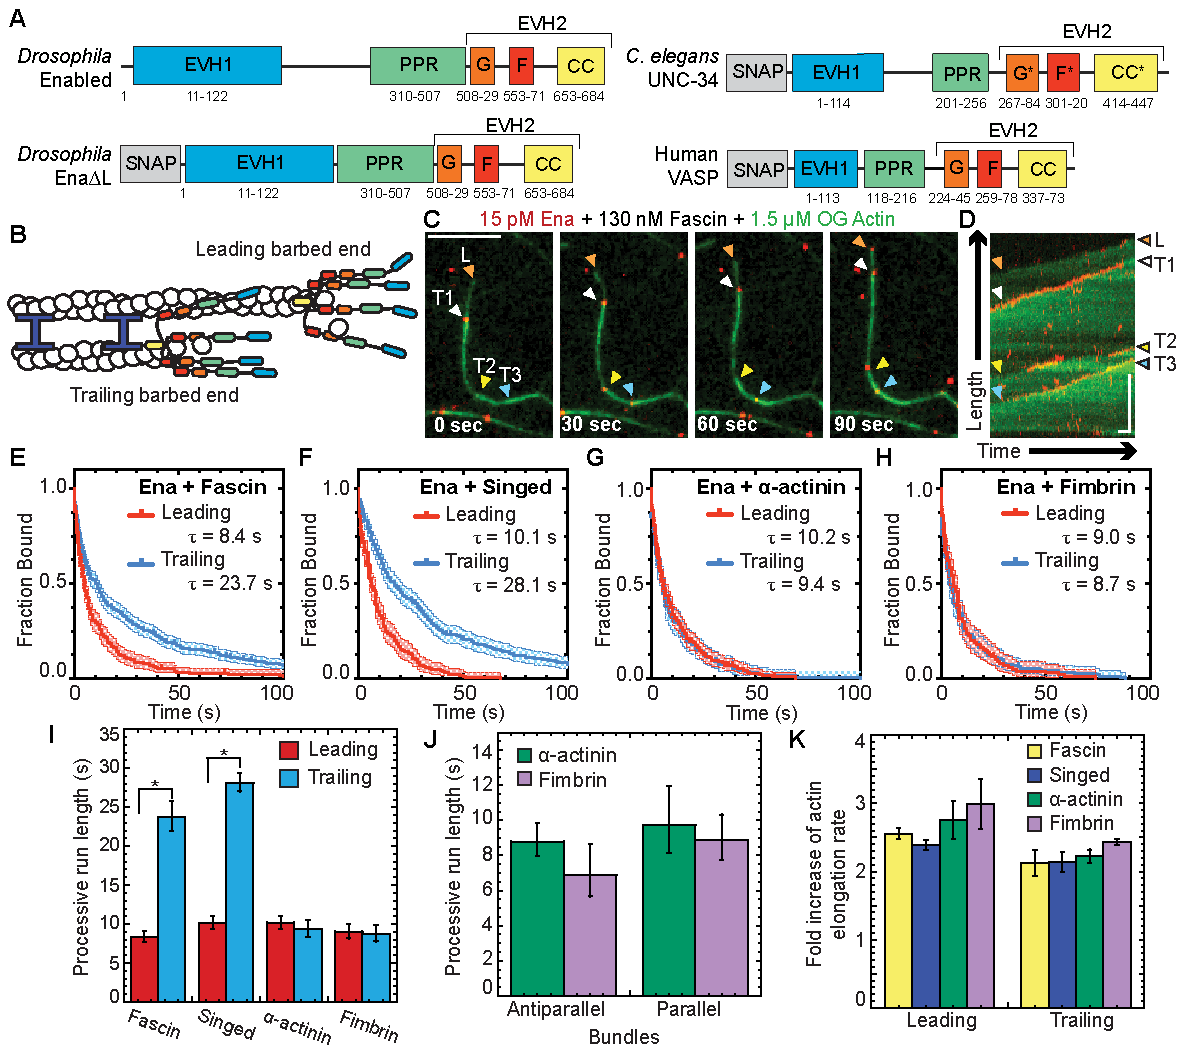
\includegraphics[width=\textwidth]{img/ch02/Figure_1_elife.pdf}
\caption[Ena has enhanced processivity on F-actin bundles formed specifically by fascin.]{\textbf{Ena has enhanced processivity on F-actin bundles formed specifically by fascin.} (A) Ena/VASP domain organization and constructs used for Ena, UNC-34, and VASP: Self-labeling tag (SNAP), Ena/VASP homology domain 1 (EVH1), polyproline region (PPR), Ena/VASP homology domain 2 (EVH2) includes G-actin binding domain (G), F-actin binding domain (F), coiled coil region (CC). *Putative domain. Two-color TIRFM visualization of 1.5 $\mu$M Mg-ATP-actin (15\% Oregon green-actin) with 15 pM SNAP(549)-Ena$\Delta$L and unlabeled 130 nM human fascin, 250 nM fly fascin Singed, 125 nM $\alpha$-actinin, or 100 nM fimbrin.  (B) Cartoon Ena/VASPs bound to leading and trailing barbed ends in a fascin bundle. (C and D) Representative experiment of OG-actin with SNAP(549)-Ena$\Delta$L and fascin. Arrows indicate leading (orange), 1st trailing (white), 2nd trailing (yellow) and 3rd trailing (blue) barbed ends. (C) Merged time-lapse micrographs. Scale bar, 5 $\mu$m. (D) Merged kymograph of filament length (scale bar, 5 $\mu$m) over time (time bar, 10 s).}
\label{fig:ena-bundlers}
\end{figure}

% Continues caption on next page. Requires package ccaption.
\begin{figure}[!htb]
  \contcaption{(continued) (E-H) Kaplan-Meier curves representing average processive run lengths ($\tau$) for Ena with (E) fascin, (F) Singed, (G) $\alpha$-actinin, or (H) fimbrin on leading (red) and trailing (blue) barbed ends. Error bars, 95\% CI. n $\geq$ 127. (I) Average processive run lengths for leading (red) and trailing (blue) barbed ends shown in E-H for 2-filament bundles with fascin, Singed, $\alpha$-actinin, or fimbrin. P values (*$<$0.0001). Error bars, 95\% CI. (J) Average processive run lengths for antiparallel and parallel 2-filament $\alpha$-actinin (green) or fimbrin (purple) bundles. Error bars, 95\% CI. n $\geq$ 64. (K) Fold increase of barbed end elongation rates of Ena on fascin (yellow), Singed (blue), $\alpha$-actinin (green), or fimbrin (purple) bundled filaments. Error bars, SEM. n $\geq$ 5 barbed ends from at least 2 movies.}
\end{figure}

\begin{table}[hbtp]
\footnotesize
\centering 
\begin{tabulary}{1.0\textwidth}{C C C C C C C C C}
\toprule Ena\slash VASP & Bundling Protein & Leading\textsuperscript{a} (s) & Trailing\textsuperscript{a} (s) & L/T p-value\textsuperscript{b} & 1 fil.\textsuperscript{c} (s) &  1 fil.\textsuperscript{c} (s) & 1 fil.\textsuperscript{c} (s) & 1/2/$\geq$3 p-value\textsuperscript{d} \\ \midrule 
Ena Tetramer & Fascin & 8.4 [7.7,9.1] (254) & 23.7 [22.0,25.8] (511) & ${<0.0001}$ & 8.9 [7.5,10.6] (107) & 16.8 [14.3,19.7] (201) & 26.0 [23.7,28.6] (308) & ${<0.0001}$ \\ 
Ena Tetramer & Singed & 10.1 [9.4,11.0] (184) & 28.1 [27.0,29.4] (328) & ${<0.0001}$ & 10.0 [9.2,10.8] (98) & 21.7 [20.4,23.3] (155) & 32.3 [31.0,33.6] (176) & ${<0.0001}$ \\ 
Ena Tetramer & $\alpha$-actinin & 10.2 [9.5,11.1] (284) & 9.4 [8.4,10.5] (176) & 0.64 & 9.1 [8.3,10.2] (165) & 8.9 [7.7,10.6] (116) & 8.7 [7.8,9.9] (60) & 0.56 \\
Ena Tetramer & Fimbrin & 9.0 [8.2,10.0] (127) & 8.7 [7.7,10.0] (183) & 0.91 & 8.2 [7.1,9.8] (63) & 7.6 [6.6,9.1] (121) & 10.2 [8.6,12.6] (64) & 0.33 \\
VASP Tetramer & Fascin & 1.2 [0.9,1.6] (213) & 3.3 [3.1,3.5] (348) & ${<0.0001}$ & 1.0 [0.7,1.8] (123) & 2.6 [2.4,2.9] (207) & 4.2 [3.9,4.4] (143) & ${<0.0001}$ \\
VASP Tetramer & Singed & 1.0 [0.7,1.5] (187) & 3.5 [3.2,3.8] (463) & ${<0.0001}$ & 0.9  [0.6, 1.6] (118) & 2.8 [2.6,3.2] (224) & 4.1 [3.7,4.7] (220) & ${<0.0001}$ \\
UNC-34 Tetramer & Fascin & 1.7 [1.4,2.2] (82) & 3.7 [3.4,4.0] (266) & ${<0.0001}$ & 1.2 [0.9,1.8] (65) & 2.9 [2.7,3.3] (123) & 3.9 [3.5,4.5] (144) & ${<0.0001}$ \\
Ena Trimer & Fascin & 6.2 [5.6,6.9] (322) & 9.8 [9.2,10.4] (299) & ${<0.0001}$ & 5.3 [4.7,6.1] (151) & 8.9 [8.3,9.6] (206) & 11.2 [10.2,12.6] (93) & ${<0.0001}$ \\
Ena Dimer & Fascin & 1.3 [1.0,1.7] (376) & 1.8 [1.5,2.4] (418) & 0.01 & 1.2 [0.9,1.9] (197) & 1.5 [1.2,2.0] (261) & 2.5 [1.9,3.8] (122) & 0.03 \\
\bottomrule
\end{tabulary}
\caption[Comparison of Ena/VASP proteins' residence time on various bundled F-actin.]{\textbf{Comparison of Ena/VASP proteins' residence time on various bundled F-actin.} \\
   \textsuperscript{a} Values of average processive lifetime (s) [95\%CI] (n) where n is the number of Ena/VASP binding events measured in at least three movies for Leading or Trailing barbed ends.\\
   \textsuperscript{b} Log Rank p-value comparing Leading and Trailing average processive lifetime. \\
   \textsuperscript{c} Values of average processive lifetime (s) [95\%CI] (n) where n is the number of Ena/VASP binding events measured in at least three movies for 1 filament (fil.), 2 filaments, or greater than or equal to 3 filaments barbed ends. \\
   \textsuperscript{d} Log Rank p-value comparing 1 filament, 2 filaments, or greater than or equal to 3 filaments average processive lifetime.}
\label{tab:ena-processive}
\end{table}

\subsection{Ena's residence time is not enhanced on trailing barbed ends of fimbrin and \texorpdfstring{$\alpha$}{a}-actinin bundles}\label{ena-processive-fimbrin-aact}

To determine if diverse bundle architectures are similarly sufficient to enhance Ena's processivity on trailing barbed ends, we tested the effect of bundling proteins with distinct properties (fimbrin and $\alpha$-actinin, see introduction). First, we measured elongation rates of Ena-bound leading and trailing barbed ends of filaments bundled by human fascin, fly fascin Singed, $\alpha$-actinin, or fimbrin. Two-color TIRFM visualization of control and Ena-bound barbed ends revealed a similar fold increase in Ena-mediated actin elongation for leading (\mytilde2.2- to 3-fold) and trailing (\mytilde2- to 2.5-fold) barbed ends with all four bundling proteins (Figures \ref{fig:ena-bundlers}K, \ref{fig:bulk-elongation}, Tables \ref{tab:ena-elongation}, \ref{tab:ena-p-elongation-bundlers}). Therefore, Ena's barbed end elongation enhancement is bundling protein independent. 

\begin{figure}
\centering
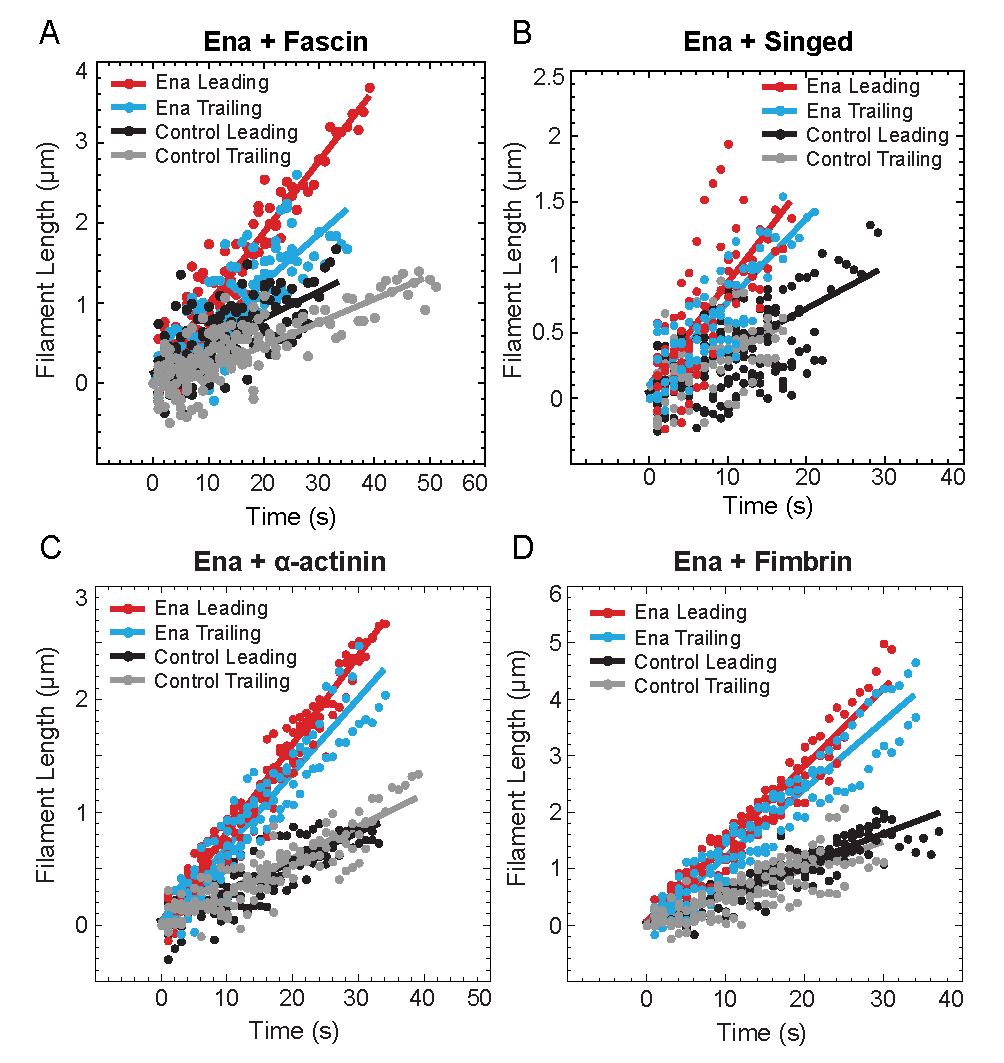
\includegraphics[width=14cm]{img/ch02/bulk_elongation_thesis.pdf}
\caption[Bulk elongation shows average elongation rates of Ena-bound and control filaments.]{\textbf{Bulk elongation show average elongation rates of Ena-bound and control filaments.} Scatter plots fit with a linear equation for the length of control filaments or Ena-bound filaments over time in the presence of 15 pM SNAP(549)-Ena$\Delta$L with either (A) 130 nM human fascin, (B) 250 nM fly fascin Singed, (C) 125 nM $\alpha$-actinin, or (D) 100 nM fimbrin. The linear fit gives the bulk elongation rate.}
\label{fig:bulk-elongation}
\end{figure}

Conversely, Ena's enhanced processivity on trailing barbed ends is specific to fascin bundles. The average processive run length on leading barbed ends with all four bundling proteins is similar, \mytilde10 sec (Figure \ref{fig:ena-bundlers}I). However, there is no enhancement of Ena's average residence time on trailing barbed ends of $\alpha$-actinin ($\tau$ = 9.4 s) or fimbrin ($\tau$ = 8.7 s) bundles (Figure \ref{fig:ena-bundlers}G-I, Table \ref{tab:ena-processive}). Therefore, F-actin bundling proteins are not universally sufficient to enhance Ena's processivity on trailing barbed ends. Although fascin exclusively forms parallel bundles, $\alpha$-actinin and fimbrin form bundles composed of filaments with mixed polarities. We therefore compared Ena's residence time on trailing barbed ends in parallel and antiparallel two-filament bundles. For both fimbrin and $\alpha$-actinin bundles, the average residence time for trailing parallel and antiparallel barbed ends is equivalent; thus, neither bundler enhances Ena's processivity (Figures \ref{fig:ena-bundlers}J, Table \ref{tab:ena-parallel}). Fimbrin can bind to single filaments \citep{skau_actin_2011}, so to control for potential hindrance of Ena/VASP association with F-actin by fimbrin binding to single filaments we tested a low concentration of fimbrin that could still bundle (Figure \ref{fig:ena-low-fim}). We found that even with low concentrations of fimbrin that there was no enhancement of Ena processivity. Therefore, neither "fascin-like" filament spacing (8-10 nm) nor polarity (parallel) of actin filaments within bundles is sufficient to facilitate increased processivity on trailing barbed ends. Given that Ena's \mytilde3-fold enhancement of processivity on trailing barbed ends is specific to fascin, different bundling proteins could regulate Ena's specific activity for different F-actin networks. 

\begin{table}[hbtp]
\centering 
\begin{tabulary}{1.0\textwidth}{C C C C C C C C C}
\toprule Ena\slash VASP & Bundling ${\textup{Protein}}$ & Bound Leading\textsuperscript{a} (sub/s) & Bound Trailing\textsuperscript{a} (sub/s) & Control Leading\textsuperscript{b} (sub/s) &  Control Trailing\textsuperscript{b} (sub/s)  &  Fold Change Leading\textsuperscript{c} & Fold Change Trailing\textsuperscript{c} & n\textsuperscript{d} \\ \midrule 
Ena Tetramer & Fascin & 25.6 $\pm$0.8 & 16.8 $\pm$1.1 & 10.0 $\pm$1.0 & 7.9 $\pm$0.2 & 2.56 $\pm$0.08 & 2.1 $\pm$0.2 & 2 \\ 
Ena Tetramer & Singed & 22.4 $\pm$0.6 & 20.0 $\pm$0.1 & 10.0 $\pm$0.9 & 10.0 $\pm$0.2 & 2.24 $\pm$0.06 & 2.00 $\pm$0.02 & 2 \\ 
Ena Tetramer & ${\alpha\mhyphen\textup{actinin}}$ & 27.6 $\pm$2.7 & 25.43 $\pm$0.03 & 10.0 $\pm$0.2 & 11.5 $\pm$0.5 & 2.8 $\pm$0.3 & 2.2 $\pm$0.1 & 2 \\
Ena Tetramer & ${\textup{Fimbrin}}$ & 29.9 $\pm$3.7 & 21.9 $\pm$1.0 & 10.0     $\pm$0.1 & 9.0 $\pm$0.3 & 3.0 $\pm$0.4 & 2.43 $\pm$0.04 & 2 \\
VASP Tetramer & Fascin & 23.6 $\pm$3.9 & 18.8 $\pm$4.6 & 10.0 $\pm$1.4 & 8.0 $\pm$0.5 & 2.4 $\pm$0.4 & 2.4 $\pm$0.7 & 2 \\
${\textup{UNC}\mhyphen34}$ Tetramer & Fascin & 27.2 $\pm$2.3 & 20.2 $\pm$3.4 & 10.0 $\pm$1.8 & 8.0 $\pm$1.5 & 2.7 $\pm$0.2 & 2.7 $\pm$0.9 & 2 \\
Ena Trimer & Fascin & 17.4 $\pm$1.3 & 14.1 $\pm$0.8 & 10.0 $\pm$0.2 & 8.70 $\pm$0.05 & 1.7 $\pm$0.1 & 1.6 $\pm$0.1 & 2 \\
Ena Dimer & Fascin & 14.5 $\pm$0.2 & 14.1 $\pm$2.2 & 10.0 $\pm$0.2 & 9.8 $\pm$0.9 & 1.45 $\pm$0.02 & 1.5 $\pm$0.4 & 2 \\
\bottomrule
\end{tabulary}
\caption[Comparison of actin elongation rates with and without (control) Ena/VASP bound.]{\textbf{Comparison of actin elongation rates with and without (control) Ena/VASP bound.} \\
   \textsuperscript{a} Normalized actin elongation rate (sub/s) of Ena/VASP bound Leading or Trailing barbed ends to Control Leading.\\
   \textsuperscript{b} Normalized actin elongation rate (sub/s) of Ena/VASP free Leading or Trailing barbed ends to Control Leading.\\
   \textsuperscript{c} Fold change in actin elongation rate of Ena/VASP bound over Ena/VASP free Leading or Trailing barbed ends.\\
   \textsuperscript{d} n is the number of movies analyzed. Each movie had at least five filaments with at least 50 length measurements for each movie.}
\label{tab:ena-elongation}
\end{table}

\begin{table}[!htb]
\centering
\begin{tabular}{ c c c c c }
\toprule 
Leading\slash Trailing\textsuperscript{a} & Fascin & Singed & $\alpha$-actinin & Fimbrin \\
\midrule
Fascin & 1 / 1 & 0.3 / 1 & 0.6 / 0.7 & 0.4 / 0.3 \\
Singed & 0.3 / 1 & 1 / 1 & 0.4 / 0.7 & 0.3 / 0.3 \\
$\alpha$-actinin & 0.6 / 0.7 & 0.4 / 0.7 & 1 / 1 & 0.7 / 0.3 \\
Fimbrin & 0.4 / 0.3 & 0.3 / 0.3 & 0.7 / 0.3 & 1 / 1 \\
\bottomrule
\end{tabular}
\caption[p-values for comparisons of fold change in actin elongation rate with Ena on different bundling proteins for both leading and trailing filaments.]{\textbf{p-values for comparisons of fold change in actin elongation rate with Ena on different bundling proteins for both leading and trailing filaments.} \\
\textsuperscript{a} p-values from student's two-tailed t-test with unequal variance between fold change of actin elongation rates when Ena is bound to the Leading or Trailing barbed end.}
\label{tab:ena-p-elongation-bundlers}
\end{table}

\begin{figure}[ht]
\centering
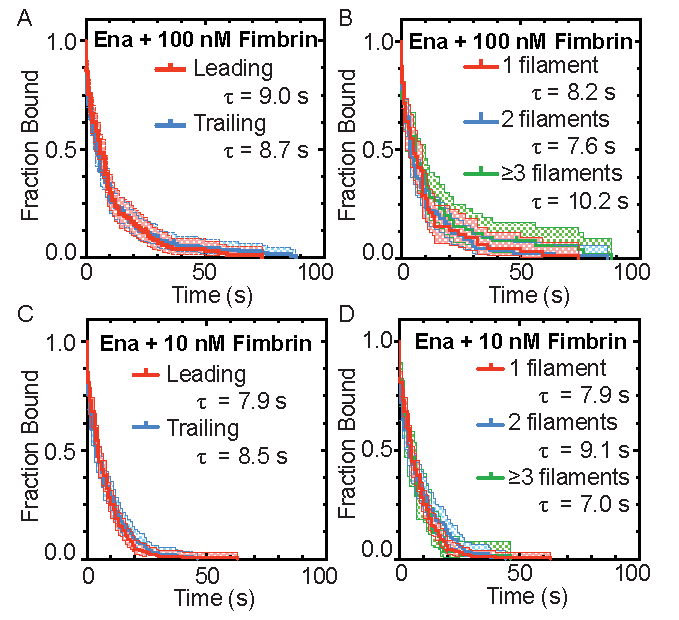
\includegraphics[width=10cm]{img/ch02/low_fimbrin.pdf}
\caption[Low concentrations of fimbrin also do not enhance Ena processivity.]{\textbf{Low concentrations of fimbrin also do not enhance Ena processivity.} Kaplan-Meier curves representing average processive run lengths ($\tau$) for Ena with (A-B) 100 nM fimbrin or (C-D) 10 nM fimbrin on (A,C) leading (red) and trailing (blue) barbed ends or further separated into (B,D) single filaments (red), or bundles with 2 (blue) and $\geq$3 (green) filaments. Error bars, 95\% CI. n $\geq$ 58.  Kaplan-Meier curve in (A) also shown in Figure \ref{fig:ena-bundlers}H.}
\label{fig:ena-low-fim}
\end{figure}

\begin{table}
\centering
\begin{tabular}{ c c c c c }
\toprule 
Ena\slash VASP & Bundling Protein & Parallel\textsuperscript{a} (s) & Antiparallel\textsuperscript{a} (s) & A/P p-value\textsuperscript{b} \\
\midrule
Ena Tetramer & Fascin & 16.8 [14.3,19.7] (201) & N/A & N/A \\
Ena Tetramer & Singed & 21.7 [20.4,23.3] (155) & N/A & N/A \\
Ena Tetramer & $\alpha$-actinin & 9.7 [8.1,12.0] (77) & 8.8 [8.0,9.8] (90) & 0.52 \\
Ena Tetramer & Fimbrin & 8.9 [7.7,10.4] (64) & 6.9 [5.7,8.7] (106) & 0.53 \\
\bottomrule
\end{tabular}
\caption[Comparison of Ena/VASP proteins' residence time on parallel and antiparallel bundled F-actin.]{\textbf{Comparison of Ena/VASP proteins' residence time on parallel and antiparallel bundled F-actin.} \\
\textsuperscript{a} Values of average processive lifetime (s) [95\%CI] (n) where n is the number of Ena/VASP binding events measured in at least three movies for parallel or antiparallel barbed ends on 2-filament bundles. Fascin results are equal to the values in 2 filaments because fascin only makes parallel bundles. \\
\textsuperscript{b} Log Rank p-value comparing average processive lifetime trailing barbed ends in parallel and antiparallel bundles.
}
\label{tab:ena-parallel}
\end{table}

\subsection{Ena's processive run length increases with bundle size}\label{ena-bundle-size}

Filopodia are composed of \mytilde10-30 actin filaments bundled by fascin \citep{svitkina_mechanism_2003,faix_making_2006}, suggesting an avidity mechanism where enhanced processivity depends on Ena simultaneously associating with a barbed end and sides of neighboring filaments. To test whether the number of filaments in a fascin bundle positively correlates with processive run length, we determined the dependence of Ena's enhanced processivity on fascin bundle size (Figure \ref{fig:ena-filaments}A). Average run lengths on trailing barbed ends (Figure \ref{fig:ena-bundlers}E-F) was thereby parsed into 2-filament bundles or 3- or more filament bundles for both human and fly fascin (Figure \ref{fig:ena-filaments}B-D, Table \ref{tab:ena-processive}). Ena's average residence time on trailing barbed ends of a 2-filament bundle ($\tau_{fascin}$ = 16.8 s, $\tau_{Singed}$ = 21.7 s) is \mytilde2-fold longer than on single filament barbed ends ($\tau_{fascin}$ = 8.9 s, $\tau_{Singed}$ = 10.0 s). Furthermore, there is an additional \mytilde1.5-fold increase in processivity when Ena is bound to trailing barbed ends of 3- or more filament bundles ($\tau_{fascin}$ = 26.0 s, $\tau_{Singed}$ = 32.2 s) (Figure \ref{fig:ena-filaments}D). Therefore, consistent with an avidity effect, Ena's processivity increases with the number of fascin-bundled filaments. 

\begin{figure}
\centering
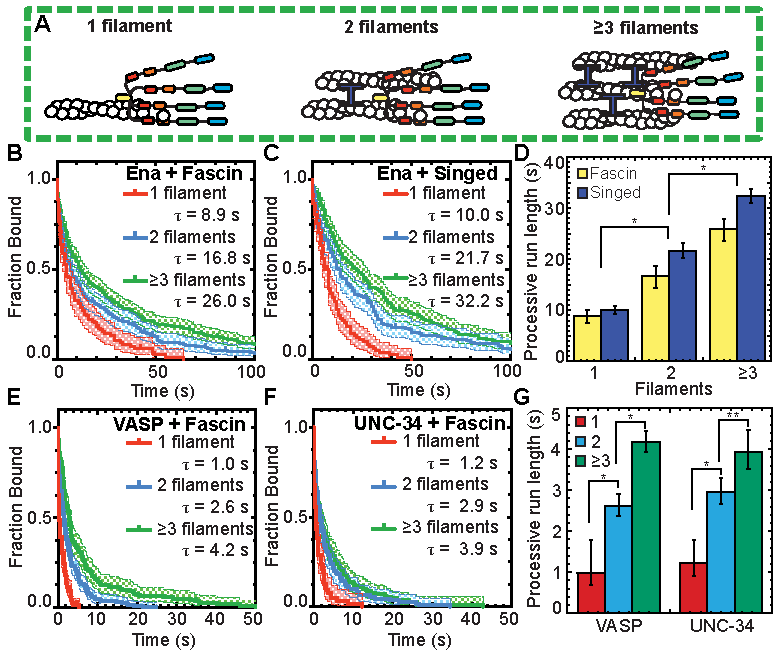
\includegraphics[width=\textwidth]{img/ch02/Figure_2_elife.pdf}
\caption[Ena/VASP's processive run length increases with the number of filaments in a fascin bundle.]{\textbf{Ena/VASP's processive run length increases with the number of filaments in a fascin bundle.} (A) Cartoons of Ena/VASP on a single filament and 2- and 3-filament fascin bundles. (B-G) Two-color TIRFM visualization of 1.5 $\mu$M Mg-ATP-actin (15\% Oregon green-actin) with fly SNAP(549)-Ena$\Delta$L (red), human SNAP(549)-VASP or worm SNAP(549)-UNC-34 and unlabeled 130 nM human fascin or 250 nM Singed as indicated. (B and C) Kaplan-Meier curves representing average processive run lengths ($\tau$) for 15 pM Ena with (B) fascin or (C) Singed on single filaments (red), or bundles with 2 (blue) and $\geq$3 (green)  filaments. Error bars, 95\% CI. n $\geq$ 98. (D) Average processive run lengths for increasing number of filaments in fascin (yellow) or Singed (blue) bundles shown in B and C. Error bars, 95\% CI. P values (*$<$0.0001). (E and F) Kaplan-Meier curves representing run lengths ($\tau$) for (E) 25 pM VASP or (F) 18 pM UNC-34 with fascin on single filaments (red), or bundles with 2 (blue) and $\geq$3 (green) filaments. Error bars, 95\% CI. n $\geq$ 60. (G) VASP and UNC-34 average processive run lengths for increasing number of filaments in fascin bundles shown in E and F. Error bars, 95\% CI. P values (*$<$0.0001).}
\label{fig:ena-filaments}
\end{figure}

\subsection{Human VASP and worm UNC-34 also have enhanced processive properties on fascin bundles}\label{vasp-unc34-processive}

To determine whether enhanced processivity on fascin-bundled trailing filament barbed ends is conserved among Ena/VASP family members, we extended our analysis to human VASP and worm UNC-34 (Figure \ref{fig:ena-bundlers}A). Human VASP is a well-characterized Ena/VASP protein \citep{bachmann_evh2_1999,chereau_understanding_2006,breitsprecher_clustering_2008,pasic_ena/vasp_2008,hansen_vasp_2010}, whereas UNC-34 had not yet been biochemically characterized in vitro despite multiple in vivo studies \citep{sheffield_c._2007,fleming_role_2010,havrylenko_wave_2015}. 

For our initial characterization of the three homologs, we measured the affinity for barbed ends and effect on actin elongation for Ena, VASP, and UNC-34. Initially, the effect of Ena/VASP homologs on actin elongation rates and their apparent affinity (Kd, app) for barbed ends was determined by single-color TIRFM visualization of spontaneous assembly of 1.5 $\mu$M Mg-ATP-actin (15\% Oregon Green) over a range of concentrations for each unlabeled Ena/VASP homolog (Figure \ref{fig:ena-homologs}A-F). All three Ena/VASP homologs increase actin elongation by a similar amount, \mytilde1.6- to \mytilde2.7-fold, at or near saturating conditions but have somewhat varying affinities for actin filament barbed ends ranging from 3.2 nM (Ena) to 6.7 nM (UNC-34) to 12.2 nM (VASP) (Figure \ref{fig:ena-homologs}F). Likewise, bulk seeded pyrene actin assembly assays also show that all three Ena/VASP homologs increase actin elongation rates by similar amounts, and fits of assembly rate over a range of Ena/VASP concentrations revealed apparent affinities for barbed ends ranging from 0.7 nM (Ena) to 10.2 nM (UNC-34) to 10.8 nM (VASP) (Figure \ref{fig:ena-homologs}G-H). We then used two-color TIRFM visualizations of red-labeled Ena, VASP, and UNC-34 on fascin bundles to measure actin elongation rates of Ena/VASP-bound leading and trailing barbed ends (Figure \ref{fig:ena-homologs}I). All three Ena/VASP homologs similarly increase actin elongation \mytilde2- to 3-fold on both leading and trailing barbed ends (Figure \ref{fig:ena-homologs}J, Tables \ref{tab:ena-p-elongation-bundlers}, \ref{tab:ena-p-elongation-homologs}). Enhancement of actin elongation rates by Ena and VASP are similar to previously reported values \citep{hansen_vasp_2010,winkelman_ena/vasp_2014,bruhmann_distinct_2017} and the actin elongation properties of UNC-34 are in good agreement with the other homologs. Therefore, though Ena, VASP, and UNC-34 vary in their barbed end affinity, they all similarly increase the actin elongation rate of both leading and trailing barbed ends of fascin-bundled filaments.

\begin{figure}
\centering
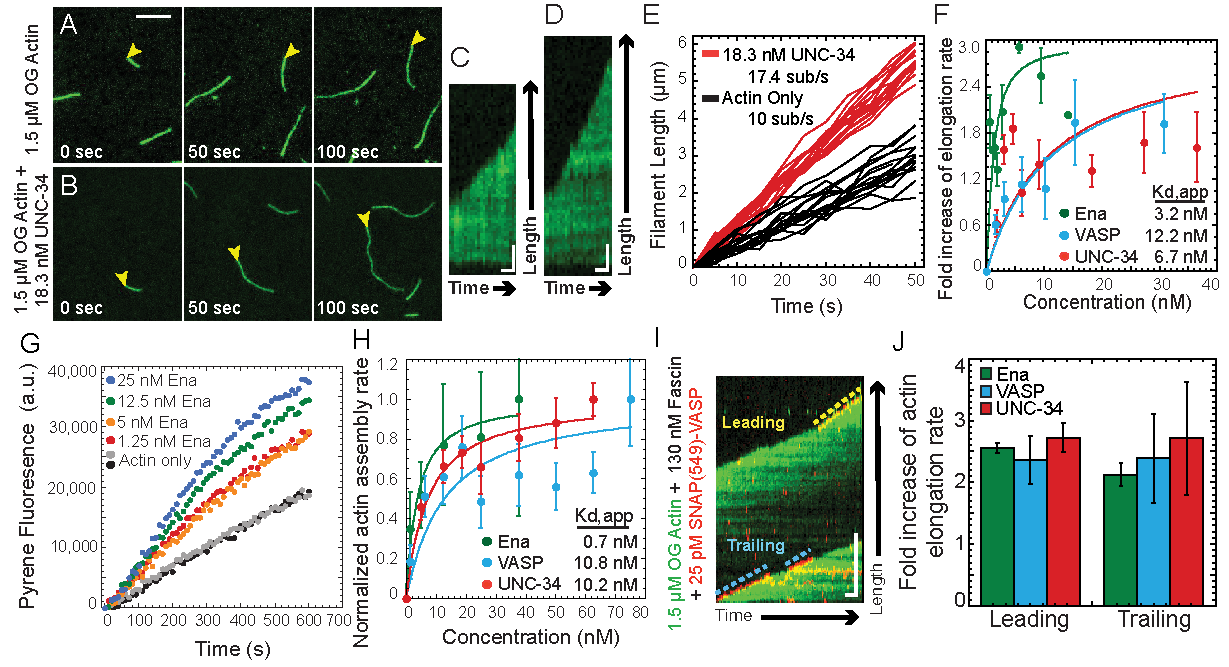
\includegraphics[width=\textwidth]{img/ch02/Supp_Figure_1.pdf}
\caption[Ena/VASP homologs have generally conserved processive actin elongation properties.]{\textbf{Ena/VASP homologs have generally conserved processive actin elongation properties.} (A-F) Single-color TIRFM of the spontaneous assembly of 1.5 $\mu$M Mg-ATP-actin (15\% Oregon Green) with worm UNC-34, fly Ena, and human VASP. (A and B) Time-lapse micrographs (scale bar, 5 $\mu$m), and (C and D) corresponding kymographs (scale bar, 1 $\mu$m; time bar, 5 s) for (A and C) actin alone or with (B and D) 18 nM UNC-34. Yellow arrowheads indicate barbed ends. (E) Length of individual filaments over time for actin only (black) and UNC-34 (red). (F) Fold increase in elongation rate over increasing concentration of Ena (green), VASP (blue), and UNC-34 (red). Curve fits revealed the indicated apparent dissociation constants (Kd, app) of Ena/VASP for the barbed end. $n \geq 5$ filaments for at least 2 movies. (G and H) Seeded assembly: addition of 0.5 $\mu$M Mg-ATP-actin monomers (20\% pyrene-labeled) to the barbed end of 0.5 $\mu$M preassembled actin filaments. (G) Time course of seeded assembly alone (black and gray) or with a range of Ena concentrations. (H) Dependence of the initial barbed end assembly rate on Ena/VASP concentration. Curve fits revealed the indicated apparent dissociation constants (Kd, app) of Ena/VASP for the barbed end. Error, SEM. $n \geq 3$. (I and J) Two-color TIRFM visualization of 1.5 $\mu$M Mg-ATP-actin (15\% Oregon Green) with 25 pM SNAP(549)-VASP, 18 pM SNAP(549)-UNC-34 or 15 pM SNAP(549)-Ena, and unlabeled 130 nM human fascin. (I) Kymograph of leading and trailing barbed ends of a fascin bundle with SNAP(549)-VASP (red) and OG actin (green). Dashed blue (trailing) and yellow (leading) lines indicate bound VASP. Scale bar, 5 $\mu$m. Time bar, 10 s. (J) Average elongation rate of leading and trailing filament barbed ends on fascin bundles with actin alone, Ena, VASP, or UNC-34. Error bars, SEM. $n \geq 5$ filaments for at least 2 movies. Elongation rate for Ena in (J) also shown in Figure \ref{fig:ena-bundlers}K.}
\label{fig:ena-homologs}
\end{figure}

\begin{table}[!htb]
\centering
\begin{tabular}{ c c c c c c }
\toprule 
Leading\slash Trailing\textsuperscript{a} & Ena\textsubscript{Tetramer} & VASP & UNC-34 & Ena\textsubscript{Trimer} & Ena\textsubscript{Dimer} \\
\midrule
Ena\textsubscript{Tetramer} & 1 / 1 & 0.7 / 0.8 & 0.6 / 0.6 & \underline{0.05} / 0.2 & \underline{0.03} / 0.3 \\
VASP & 0.7 / 0.8 & 1 / 1 & 0.5 / 0.8 & 0.3 / 0.5 & 0.3 / 0.4 \\
UNC-34 & 0.6 / 0.6 & 0.5 / 0.8 & 1 / 1 & 0.09 / 0.4 & 0.1 / 0.4 \\
Ena\textsubscript{Trimer} & \underline{0.05} / 0.2 & 0.3 / 0.5 & 0.09 / 0.4 & 1 / 1 & 0.3 / 0.8 \\
Ena\textsubscript{Dimer} & \underline{0.03} / 0.3 & 0.3 / 0.4 & 0.1 / 0.4 & 0.3 / 0.8 & 1 / 1 \\
\bottomrule
\end{tabular}
\caption[p-values for comparisons of fold change in actin elongation rate with different Ena/VASPs on both leading and trailing filaments of fascin bundles.]{\textbf{p-values for comparisons of fold change in actin elongation rate with different Ena/VASPs on both leading and trailing filaments of fascin bundles.} \\
\textsuperscript{a} p-values from student's two-tailed t-test with unequal variance between fold change of actin elongation rates when Ena/VASP is bound to the Leading or Trailing barbed end. Underlining shows p-values $\leq0.05$.}
\label{tab:ena-p-elongation-homologs}
\end{table}

To test if different Ena/VASP homologs have similarly enhanced processive properties on fascin bundles, two-color TIRFM visualization of 1.5 $\mu$M Mg-ATP-actin (15\% Oregon Green) was used to quantify the processive run lengths of fluorescently labeled VASP and UNC-34 on fascin bundles (Figure \ref{fig:ena-filaments}E-G). The average residence time of both VASP (1.0 s) and UNC-34 (1.2 s) on single filament barbed ends is \mytilde9-fold shorter than Ena (8.9 s), as expected from lower apparent affinities for barbed ends and previously reported values \citep{hansen_vasp_2010}. Yet, like Ena, both VASP and UNC-34 have \mytilde2.5-fold longer processive run lengths on trailing barbed ends of 2-filament bundles ($\tau_{VASP}$ = 2.6 s, $\tau_{UNC-34}$ = 2.9 s), with an additional \mytilde1.5-fold increase on trailing barbed ends of 3- or more filament bundles ($\tau_{VASP}$ = 4.2 s, $\tau_{UNC-34}$ = 3.9 s) (Figure \ref{fig:ena-filaments}E–G, Table \ref{tab:ena-processive}). Therefore, enhanced processivity on fascin-bundled trailing barbed ends is conserved from worms to flies to humans, suggesting that enhanced processivity is important for Ena/VASP's activity in cells. 

\begin{figure}
\centering
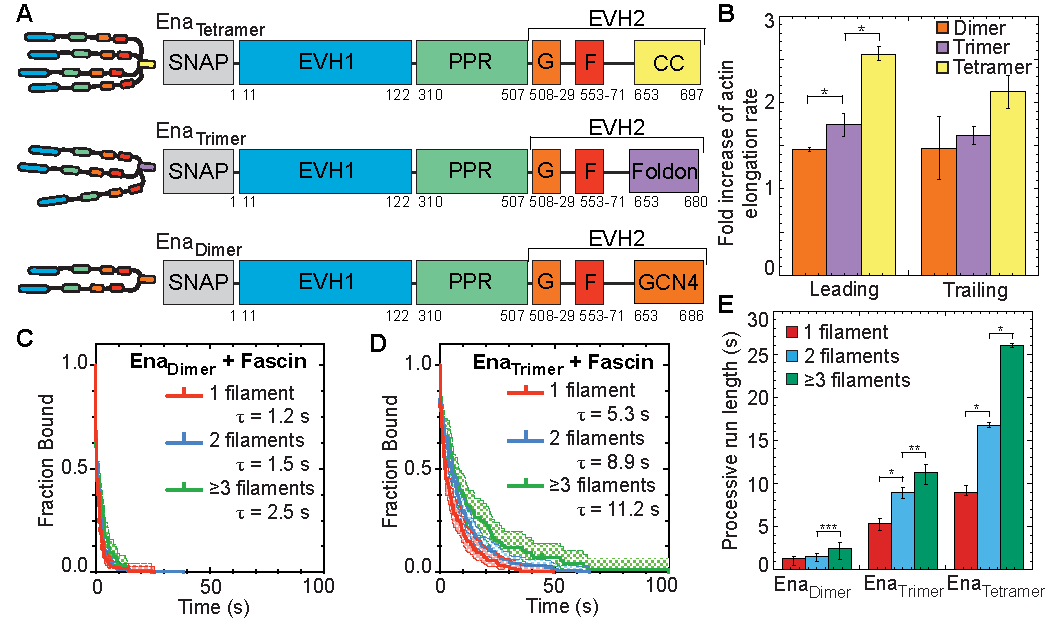
\includegraphics[width=\textwidth]{img/ch02/Figure_3_elife.pdf}
\caption[Ena's processive run length increases with the number of Ena ‘arms'.]{\textbf{Ena's processive run length increases with the number of Ena ‘arms'.} (A) Cartoon and domain organizations of Ena\textsubscript{Tetramer}, Ena\textsubscript{Trimer}, and Ena\textsubscript{Dimer}. (B-E) Two-color TIRFM visualization of 1.5 $\mu$M Mg-ATP-actin (15\% Alexa 488-actin) with indicated SNAP(549)-Ena construct and 130 nM fascin. (B) Fold increase of barbed end elongation rates of Ena\textsubscript{Dimer} (orange), Ena\textsubscript{Trimer} (purple), and Ena\textsubscript{Tetramer} (yellow). Error bars, SEM. n $\geq$ 5 barbed ends from at least 2 movies. P values (*$\leq$0.05) (C and D) Kaplan-Meier curves representing average processive run lengths ($\tau$) for (C) 50 pM MBP-SNAP(549)-Ena$\Delta$L$\Delta$CC-GCN4 or (D) 70 pM MBP-SNAP(549)-Ena$\Delta$L$\Delta$CC-Foldon with fascin on single filaments (red) or bundles with 2 (blue) and $\geq$3 (green) filaments. Error bars, 95\% CI. n $\geq$ 93. (E) Average processive run length for increasing number of Ena "arms" on single filaments (red), or fascin bundles with 2 (blue) and $\geq$3 (green) filaments shown in C and D. Error bars, 95\% CI. P values (*$<$0.05, **$<$0.0001). Ena\textsubscript{Tetramer} data in (B) and (E) was also reported in \ref{fig:ena-bundlers}K and \ref{fig:ena-filaments}D respectively. }
\label{fig:ena-arms}
\end{figure}

\subsection{Enhanced elongation and processive run length increases with the number of Ena arms}\label{ena-processive-arms}

Wildtype Ena is a tetrameric protein \citep{kuhnel_vasp_2004, winkelman_ena/vasp_2014}, with four arms that could facilitate simultaneous association with a barbed end, neighboring actin filaments, and/or actin monomers for processive elongation. Since we observed that Ena's average processive run length increases with number of fascin-bundled filaments (Figure \ref{fig:ena-filaments}), we investigated the importance of Ena's oligomeric state by measuring actin elongation and processive properties of dimeric and trimeric Ena. Dimer and trimer constructs were formed by replacing Ena's coiled-coil tetramerization domain with a GCN4 dimerization domain \citep{harbury_switch_1993} or a Foldon trimerization domain (Figure \ref{fig:ena-arms}A) \citep{guthe_very_2004, papanikolopoulou_formation_2004}; and the oligomeric state was verified by gel filtration and multi-angle light scattering (Figure \ref{fig:ena-sizes}A-C). Two-color TIRFM was used to visualize 1.5 $\mu$M Mg-ATP-actin (15\% Alexa-488 labeled) with SNAP(549)-Ena$\Delta$L$\Delta$CC-GCN4 (referred to as Ena\textsubscript{Dimer}) or SNAP(549)-Ena$\Delta$L$\Delta$CC-Foldon (referred to as Ena\textsubscript{Trimer}) on fascin bundles. First, we measured actin elongation rates of Ena-bound leading and trailing barbed ends (Figure \ref{fig:ena-arms}B, Tables \ref{tab:ena-elongation}, \ref{tab:ena-p-elongation-homologs}). While all constructs increase actin's elongation rate on both leading and trailing filaments, the fold increase is positively correlated with the number of Ena arms. Ena\textsubscript{Tetramer} has the largest enhancement of actin elongation (2.56-fold leading, 2.1-fold trailing), followed by Ena\textsubscript{Trimer} (1.74-fold leading, 1.62-fold trailing), and then Ena\textsubscript{Dimer} (1.45-fold leading, 1.46-fold trailing). 

\begin{figure}
\centering
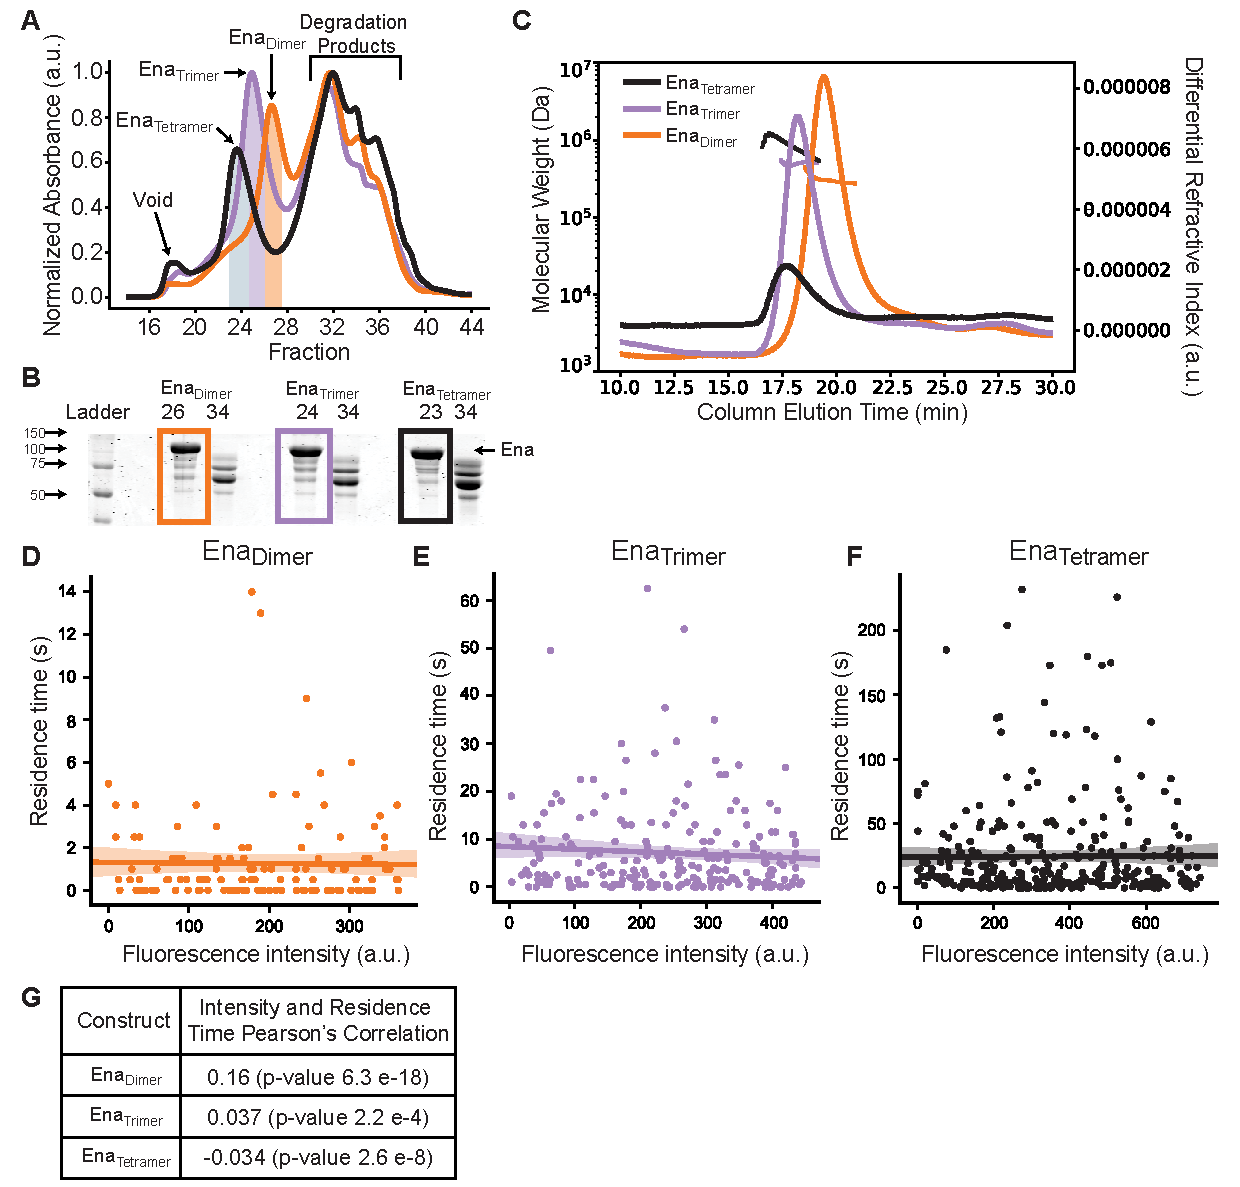
\includegraphics[width=\textwidth]{img/ch02/Supp_Figure_2_PNAS.pdf}
\caption[Ena constructs have the predicted oligomerization state.]{\textbf{Ena constructs have the predicted oligomerization state.} (A) UV traces for Ena\textsubscript{Dimer} (orange), Ena\textsubscript{Trimer} (purple), and Ena\textsubscript{Tetramer} (black) from size exclusion gel filtration using a Sepharose 6 Increase column. Peaks are labeled and fractions collected are shaded. (B) The 12.5\% SDS-PAGE of fractions from A. Fractions showing each construct are boxed. (C) Size exclusion chromatography followed by multi-angle light scattering (SEC-MALS) was used to determine the relative size of Ena\textsubscript{Dimer} (orange), Ena\textsubscript{Trimer} (purple), and Ena\textsubscript{Tetramer} (black). Dependence of (D) Ena\textsubscript{Dimer}, (E) Ena\textsubscript{Trimer}, or (F) Ena\textsubscript{Tetramer} processive run length on its respective fluorescence intensity for an individual movie. Linear correlation fit shown with 95\% CI shaded. (G) Values for the Pearson's correlation of the Ena construct fluorescence intensity and its residence time for all movies analyzed. There is no correlation between an Ena construct's intensity and its bound lifetime.}
\label{fig:ena-sizes}
\end{figure}

Similar to actin elongation rates, average processive run length is also positively correlated with the number of Ena arms (Figure \ref{fig:ena-arms}C-E). Remarkably, although reduced \mytilde10-fold compared to Ena\textsubscript{Tetramer}, Ena\textsubscript{Dimer} does remain processively associated with single filament ($\tau$ = 1.2 s), 2-filament trailing ($\tau$ = 1.5 s), and 3- or more filament trailing ($\tau$ = 2.5 s) barbed ends (Figure \ref{fig:ena-arms}C,E, Movie S3, Table \ref{tab:ena-processive}). Ena\textsubscript{Trimer} has intermediate processivity on single filament ($\tau$ = 5.3 s), 2-filament trailing ($\tau$ = 8.9 s), and 3- or more filament trailing ($\tau$ = 11.2 s) barbed ends (Figure \ref{fig:ena-arms}D,E, Table \ref{tab:ena-processive}). For each construct, the fluorescence intensity is not correlated with run length (Figure \ref{fig:ena-sizes}D-G), indicating that processive activity is not affected by Ena construct multimerization. Ena\textsubscript{Trimer}'s processive run lengths are similar to the residence time of Ena\textsubscript{Tetramer} on single filaments but are not comparably enhanced on trailing barbed ends (Figure \ref{fig:ena-arms}E). Therefore, Ena\textsubscript{Dimer} is sufficient for processive elongation, Ena\textsubscript{Trimer} is necessary for longer processive runs on single filaments, but Ena\textsubscript{Tetramer} is necessary for the longest processive runs on trailing barbed ends of fascin bundles (Figure \ref{fig:ena-arms}E). Interestingly, the avidity effect of multiple filaments in a fascin bundle is apparent even with fewer arms than the wildtype tetramer. The positive correlation between processive elongation and Ena arms is consistent with a recent study on chimeric human VASP with \textit{Dictyostelium} GAB domains on single actin filaments \citep{bruhmann_distinct_2017}. 

\begin{figure}
\centering
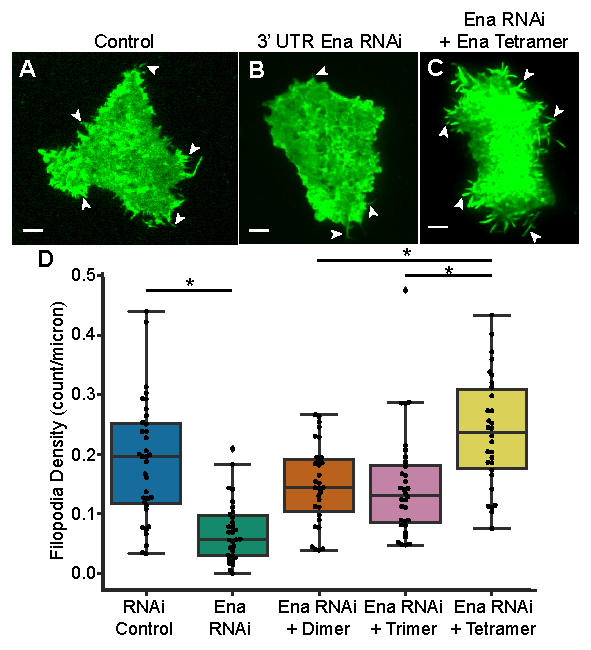
\includegraphics[width=5in]{img/ch02/Figure_4_elife.pdf}
\caption[Tetrameric Ena is necessary for proper filopodia density.]{\textbf{Tetrameric Ena is necessary for proper filopodia density.} (A-C) Representative fluorescent micrographs of D16 cells with GFP-actin for (A) control treatment, (B) Ena 3' UTR RNAi, and (C) RNAi with transfection of mCherry-Ena\textsubscript{Tetramer}. White arrows indicate representative filopodia. (D) Boxplot of filopodia density, number of filopodia per micron of cell perimeter, for control cells, Ena 3'UTR RNAi, and RNAi transfected with mCherry-Ena$\Delta$CC-GCN4 (Ena\textsubscript{Dimer}), mCherry-Ena$\Delta$CC-Foldon (Ena\textsubscript{Trimer}), and mCherry-Ena\textsubscript{Tetramer}. n = 3 with at least 10 cells for each experiment. P values (*$<$0.0005).}
\label{fig:ena-cells}
\end{figure}

\subsection{Tetrameric Ena is more efficient at forming filopodia in \textit{Drosophila} culture cells}\label{ena-fly-cells}

Ena\textsubscript{Tetramer} is significantly better at processive actin filament assembly than either Ena\textsubscript{Dimer} or Ena\textsubscript{Trimer}, where Ena\textsubscript{Tetramer} increases the actin elongation rate \mytilde2- to 2.5-fold and remains processively associated with trailing barbed ends of fascin bundles for \mytilde25 sec (Figure \ref{fig:ena-arms}B,E). To determine whether WT Ena\textsubscript{Tetramer} is therefore necessary for proper function in cells, we evaluated the ability of Ena oligomerization constructs to facilitate filopodia in ML-DmD16-c3 \textit{Drosophila} culture cells, derived from third instar larval wing discs (Figure \ref{fig:ena-cells}). We knocked down endogenous Ena with dsRNAi against the 3'UTR and then expressed mCherry-Ena (referred to as mCherry-Ena\textsubscript{Tetramer}), mCherry-Ena$\Delta$CC-GCN4 (referred to as mCherry-Ena\textsubscript{Dimer}) or mCherry-Ena$\Delta$CC-Foldon (referred to as mCherry-Ena\textsubscript{Trimer}) constructs from a constitutive pIZ plasmid (Figure \ref{fig:ena-cells}A-C). The activity of the different Ena constructs was determined by quantifying filopodia density, the number of filopodia per perimeter of the cell (Figure \ref{fig:ena-cells}D). Compared to control cells (0.19 $\pm$ 0.06 filopodia/micron), RNAi treated cells without exogenous Ena have a 2.7-fold decrease in filopodia density (0.07 $\pm$ 0.03 filopodia/micron). Strikingly, mCherry-Ena\textsubscript{Tetramer} forms significantly more filopodia (0.24 $\pm$ 0.05 filopodia/micron) compared to mCherry-Ena\textsubscript{Trimer} (0.15 $\pm$ 0.05 filopodia/micron) and mCherry-Ena\textsubscript{Dimer} (0.15 $\pm$ 0.04 filopodia/micron). There was no correlation between filopodia density and GFP-actin fluorescence or mCherry fluorescence (Figure \ref{fig:ena-expression}). Therefore, Ena tetramers facilitate the production of significantly more filopodia than dimer and trimer constructs following knockdown of endogenous Ena.

\begin{figure}
\centering
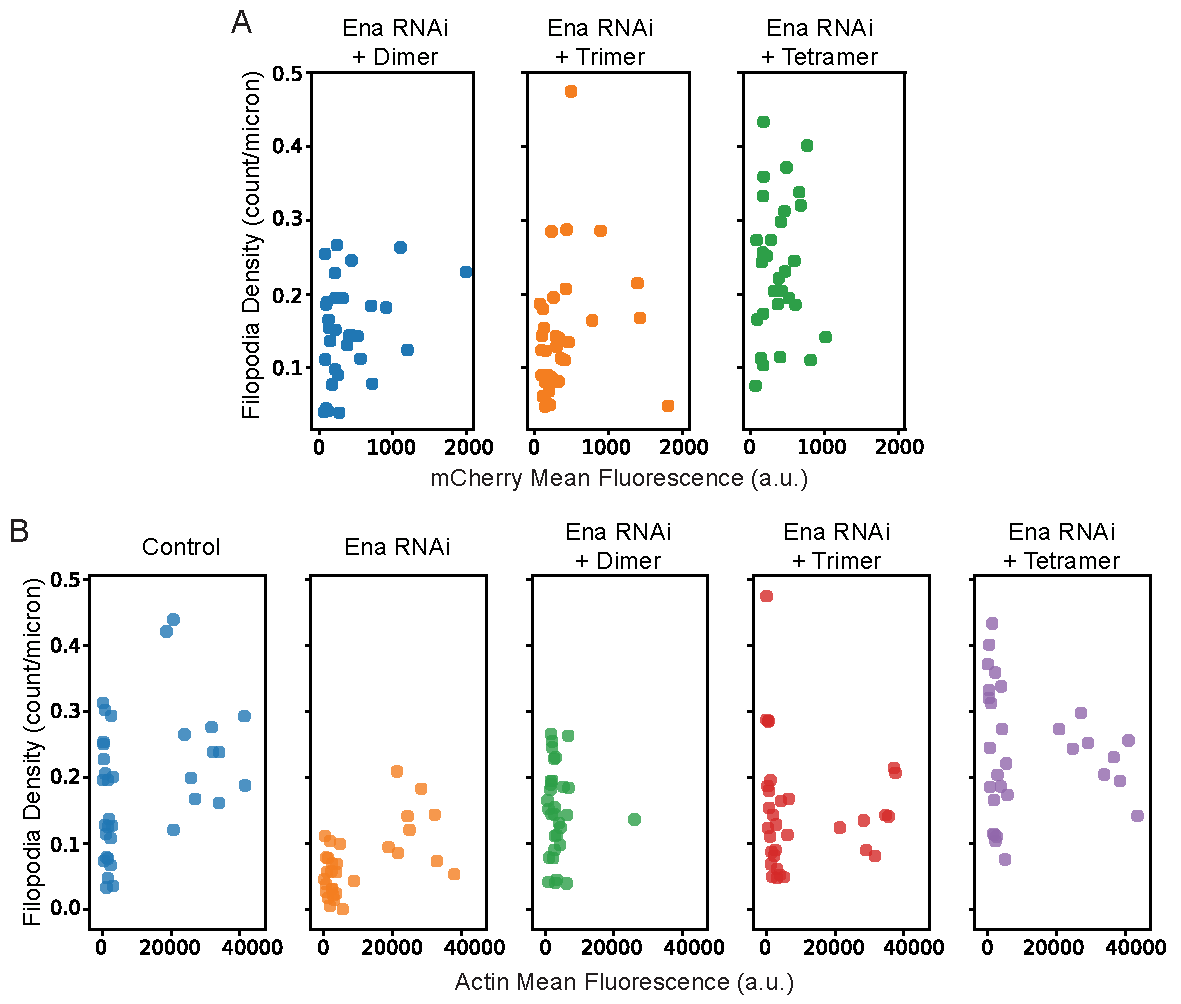
\includegraphics[width=6in]{img/ch02/Supp_Figure_3_PNAS.pdf}
\caption[D16 culture cell expression is independent of construct.]{\textbf{D16 culture cell expression is independent of construct.} (A) Dependence of filopodia density on mCherry fluorescence of RNAi treated cells transfected with mCherry-Ena\textsubscript{Dimer}, mCherry-Ena\textsubscript{Trimer}, or mCherry-Ena\textsubscript{Tetramer}. (B) Dependence of filopodia density on the GFP-actin fluorescence intensity for control or RNAi treated control and mCherry-Ena\textsubscript{Dimer}, mCherry-Ena\textsubscript{Trimer}, or mCherry-Ena\textsubscript{Tetramer} transfected cells.}
\label{fig:ena-expression}
\end{figure}

\subsection{Kinetic model of Ena shows a direct correlation between processivity and both bundle size and Ena oligomerization}\label{ena-model}

We observed that Ena's processivity depends on the number of filaments in a fascin bundle (Figure \ref{fig:ena-filaments}D) and number of Ena arms (Figure \ref{fig:ena-arms}E). Therefore, it is likely that the underlying molecular mechanism for Ena's increased processivity on trailing barbed ends depends on Ena's ability to simultaneously bind to an elongating barbed end and sides of filaments via its multiple arms (Figure \ref{fig:ena-bundlers}B). To investigate this avidity effect, we developed a kinetic model of Ena with varying number of arms, $N$, binding bundles composed of varying number of actin filaments, $n$ (Figure \ref{fig:ena-model}A, \ref{fig:ena-si-model}A). 

\begin{figure}
\centering
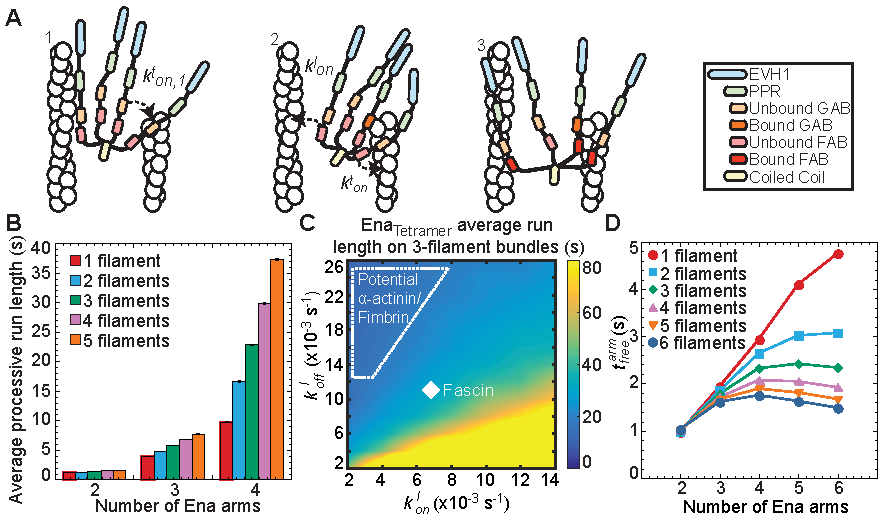
\includegraphics[width=\textwidth]{img/ch02/Figure_5_elife.pdf}
\caption[Kinetic model of Ena/VASP on actin bundles shows processivity positively correlates with both number of Ena arms and bundle size.]{\textbf{Kinetic model of Ena/VASP on actin bundles shows processivity positively correlates with both number of Ena arms and bundle size.} (A) Modeling schematics showing (from left to right). [1] An Ena arm's GAB domain binds the trailing barbed end with binding rate $k^{t}_{on,1}$. [2] Once the GAB domain is bound, the FAB domains from the other arms bind to sides of either the trailing filament ($k^{t}_{on}$) or leading filaments ($k^{l}_{on}$). [3] Arms can be bound to the trailing filament, while others bind leading filaments. (B) Bar graph of the average processive run length as a function of number of Ena arms and bundle size. Error bars, SEM. (C) Heat map showing average Ena run length in the case of 3-filament bundles and four Ena arms, with systematic variations of $k^{l}_{on}$ and $k^{l}_{off}$. Diamond denotes optimized rates for fascin bundles and region within dotted line shows potential rates for $\alpha$-actinin and fimbrin. (D) Average time between binding events ($\tau_{free}^{arm}$) for varying arm number and bundle size.}
\label{fig:ena-model}
\end{figure}

Our model considers binding and unbinding kinetics of all $N$ Ena arms on various binding sites of individual actin filaments in a bundle, which together dictate the kinetics of the Ena “molecule” as a whole (Figure \ref{fig:ena-model}A). An Ena arm initially binds to the trailing barbed end with an on rate of $k_{on,1}^{t}$ and unbinds with an off rate of $k_{off,1}^t$ (Figure \ref{fig:ena-model}A1). The remaining Ena arms are available to bind and unbind to the side of the trailing filament with a rate $k_{on}^{t}$ and $k_{off}^{t}$ or to the side of other filaments in the bundle with a rate $k_{on}^{l}$ and $k_{off}^{l}$ (Figure \ref{fig:ena-model}A2-3). A Monte Carlo algorithm was used to integrate rates of binding and unbinding of Ena arms over time as described in the SI. The model parameter $k_{on,1}^{t}$ was 0.007 s\textsuperscript{-1}, estimated using the TIRFM measured off rate of 0.109 s\textsuperscript{-1} for Ena, and an equilibrium constant of Ena for the barbed end of 0.8 nM \citep{winkelman_ena/vasp_2014}. We therefore considered the local concentration of Ena near the barbed end as 50 pM. The other model parameters were optimized using TIRFM off rates for $N\in(2,3,4)$ and $n\in(1,2,\geq3)$ (Figure \ref{fig:ena-arms}E), as described in the Supplementary Information. 

\begin{figure}
\centering
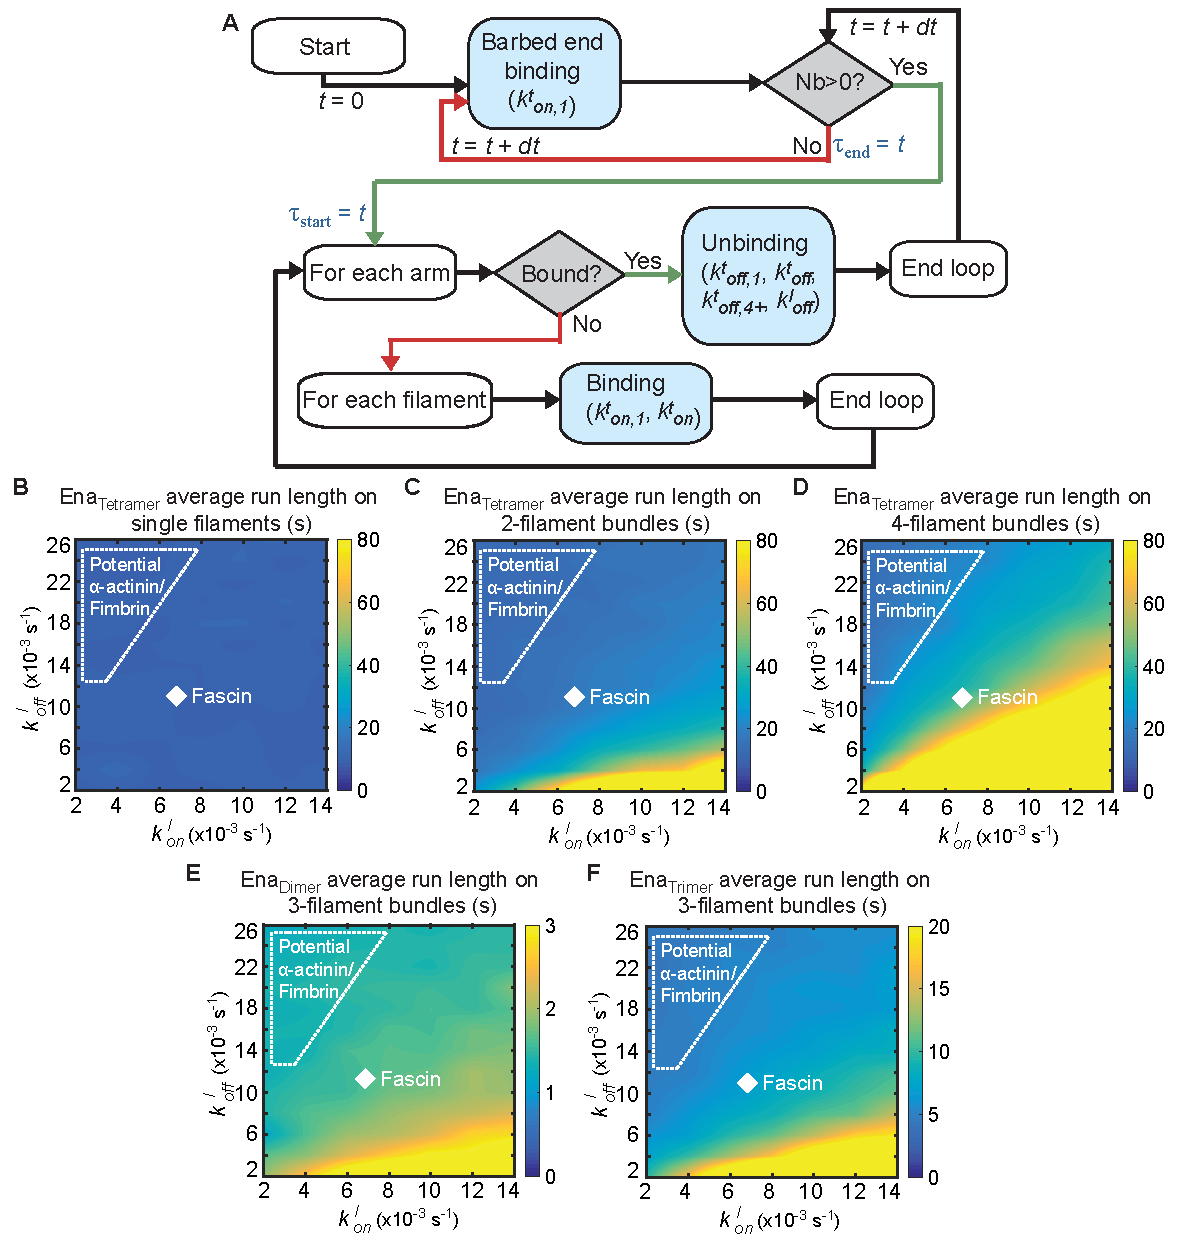
\includegraphics[width=\textwidth]{img/ch02/Supp_Figure_4_PNAS.pdf}
\caption[Kinetic model can explore different parameter spaces.]{\textbf{Kinetic model can explore different parameter spaces.} (A) Diagram showing the key steps in the algorithm. Nb represents the number of arms bound at time $t$. $\tau_{start}$ and $\tau_{end}$ mark the start and end of Ena "molecule" binding events. The processive run length $\tau$ is estimated as the average of the difference $\tau_{end} - \tau_{start}$ across several events. }
\label{fig:ena-si-model}
\end{figure}

% Continues caption on next page. Requires package ccaption.
\begin{figure}[!htb]
  \contcaption{(continued) (B – F) Heat maps showing average Ena processive run length with systematic variations of $k^{l}_{on}$ and $k^{l}_{off}$. Heat maps of average processive run length for (B) single filaments (C) 2-filament bundles or (D) 4-filament bundles with four Ena arms. These are comparable to Figure \ref{fig:ena-model}C with 3-filament bundles. Heat maps of average processive run length for 3-filament bundles with (E) two or (F) three Ena arms.}
\end{figure}

We used the model to characterize Ena's processive run length at the trailing barbed end. Increasing both the number of filaments in a bundle and the number of Ena arms increases Ena's processive run length, which strongly supports the avidity hypothesis. The modeling results are also in excellent agreement with the trends observed from our TIRFM data (Figure \ref{fig:ena-model}B). Using the model, we tested conditions over a range of both $k_{on}^{l}$ and $k_{off}^{l}$ to mimic $\alpha$-actinin and fimbrin bundles (Figure \ref{fig:ena-bundlers}I), where Ena processivity is not enhanced on trailing barbed ends (Figure \ref{fig:ena-si-model}B-F). The model shows a broad regime that results in the same average processive run length on both leading and trailing barbed ends (Figure \ref{fig:ena-model}C, dashed region). This indicates that differences between bundlers could be due to an effect on Ena's association and dissociation rates caused by differences in how CH domain bundlers and fascin bind F-actin. 

Finally, we used the model to estimate rates of Ena-mediated filament elongation. While at least one Ena arm associates with the barbed end, its other arms undergo binding and dissociation events. When free, an arm can bind G-actin from solution and transfer it to the barbed end. The elongation rate of the Ena bound filament should be proportional to the average time that individual arms are free. From the model, the average time that individual arms remain unbound while the Ena molecule is in the bound state, $\tau_{free}^{arm}$, increases with $N$, and decreases with $n$ (Figure \ref{fig:ena-model}D). This result is consistent with the TIRFM data for the fold increase of actin elongation rate due to Ena on the leading ($n=1$ in the model) and trailing barbed ends ($n>1$ in the model) (Figure \ref{fig:ena-bundlers}K, 3B).

\section{Discussion}\label{ch02-discussion}

\subsection{Ena's processivity is enhanced specifically on fascin bundles}\label{ena-discuss-specific-fascin}

Ena/VASP proteins are important processive actin elongation factors that are localized to diverse F-actin networks composed of filaments bundled by different crosslinking proteins, including fascin, fimbrin, and $\alpha$-actinin. Previously, we found that Ena takes \mytilde3-fold longer processive runs on trailing barbed ends of fascin-bundled F-actin \citep{winkelman_ena/vasp_2014}. Here we investigated the mechanism and conservation of Ena/VASP's processivity at the barbed end of single filaments and filaments bundled by different crosslinking proteins, as well as the physiological relevance of Ena/VASP tetramerization.

We found that although fly Ena's processivity is enhanced \mytilde3-fold on trailing barbed ends in fascin bundles, there is no processivity enhancement on trailing barbed ends of $\alpha$-actinin or fimbrin bundles (Figure \ref{fig:ena-bundlers}I). Fimbrin and $\alpha$-actinin use two CH domains to bundle F-actin, whereas fascin uses $\beta$-trefoil domains. Though the exact mechanism for Ena's specificity for fascin bundles remains unclear, we suggest several hypotheses. First, fascin could hold the trailing filament in a specific register with respect to the leading filament, allowing for easier Ena/VASP binding. Second, fascin's strong cooperativity \citep{yamakita_phosphorylation_1996,winkelman_fascin-_2016} could promote more rapid bundling, thereby promoting longer processive runs by keeping trailing barbed ends closer to sides of leading filaments. Third, it is also possible that Ena weakly associates with fascin, although no interaction has yet been detected. If Ena does associate with fascin, it would need to be carefully tuned because a strong interaction could pull Ena from the barbed end. 

The fourth hypothesis is based off of a result from our kinetic model, which revealed a broad region of Ena binding kinetics to sides of bundled filaments ($k_{on}^{l}$ and $k_{off}^{l}$) that could explain Ena's lack of enhanced processivity on fimbrin and $\alpha$-actinin bundles (Figure \ref{fig:ena-model}B). We used a bulk sedimentation assay to test if there is a difference in Ena's F-actin binding in the presence and absence of fascin. We used two different constructs to test the affinity, GABFAB and EVH2 (Figure \ref{fig:sedimentation}A). GABFAB contains the GAB and FAB domains and is a monomeric protein while EVH2 contains the GAB, FAB, and CC domains and is a tetramer. We saw no significant difference in either the GABFAB (Figure \ref{fig:sedimentation}B-C) or EVH2 F-actin binding (Figure \ref{fig:sedimentation}D-E). These results suggests that if there is a difference in FAB binding to the sides of bundled filaments that it cannot be measured in a bulk steady-state assay. It is also possible that Ena's on and off rates are affected by competition between Ena and the CH domain bundling proteins for similar binding sites on sides of actin filaments. 

Further studies of how fascin forms F-actin networks differently than $\alpha$-actinin and fimbrin will be required to fully elucidate the underlying molecular mechanism. However, this important observation reveals for the first time that bundling proteins and the F-actin networks they form can differentially regulate the activity of processive actin assembly factors, thereby providing a mechanism to allow Ena/VASP proteins to facilitate the assembly of diverse bundled networks with different dynamics in cells. Understanding how different bundling proteins associate with and help form specific F-actin networks in cells will therefore be of critical importance.

\begin{figure}
\centering
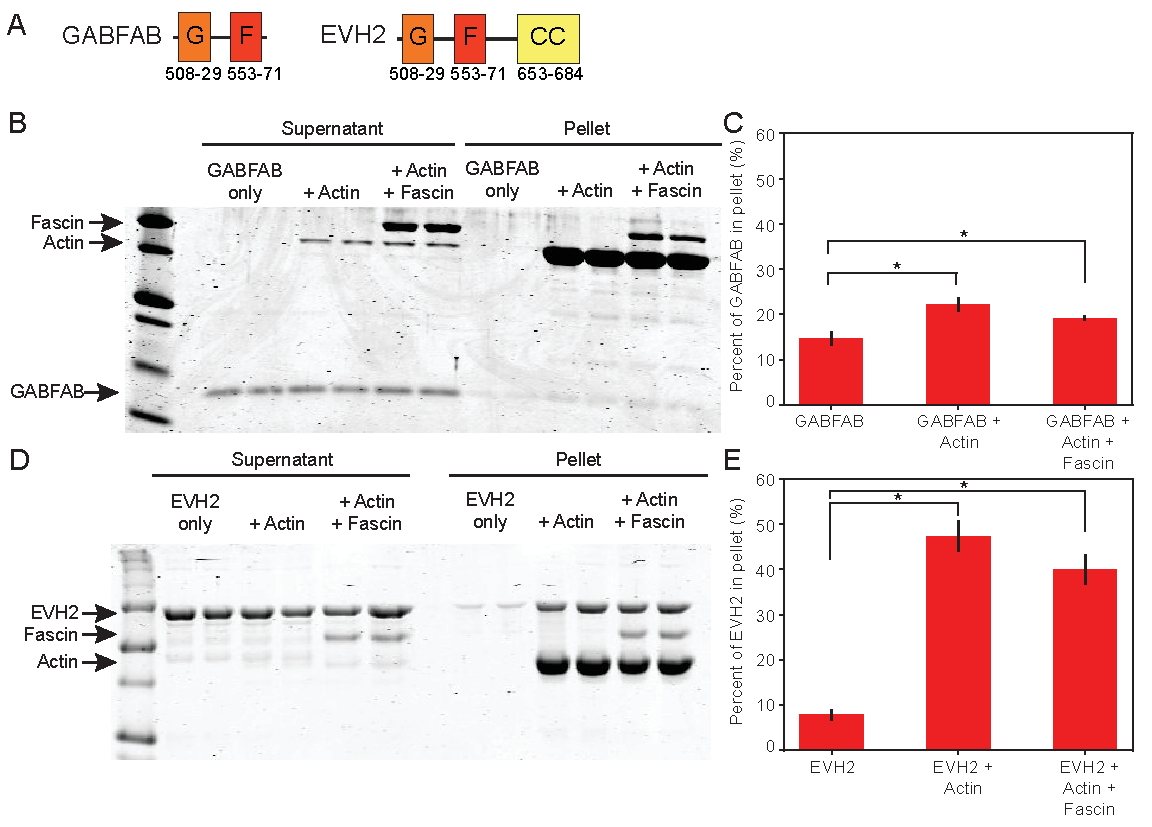
\includegraphics[width=\textwidth]{img/ch02/sedimentation_thesis.pdf}
\caption[GABFAB and EVH2 bind similarly to single filaments and fascin bundles in bulk sedimentation.]{\textbf{GABFAB and EVH2 bind similarly to single filaments and fascin bundles in bulk sedimentation.} (A) Domain organization for constructs used in sedimentation. G-actin binding domain (G), F-actin binding domain (F), coiled coil region (CC). (B) 15\% SDS-PAGE gel showing supernatant (left) and pellet (right) for the specified combination of 5 $\mu$M GABFAB, 5 $\mu$M actin, and 1 $\mu$M fascin. The reactions were done in duplicate. (C) Percent of GABFAB found in pellet for GABFAB alone, GABFAB with actin, and GABFAB with actin and fascin. Error bars, SEM. n = 8. P values (* $<0.05$). (D) 12.5\% SDS-PAGE gel showing supernatant (left) and pellet (right) for specified combinations of 2.5 $\mu$M EVH2, 5 $\mu$M actin, and 1 $\mu$M fascin. The reactions were done in duplicate. (E) Percent of EVH2 found in pellet for EVH2 alone, EVH2 with actin, and EVH2 with actin and fascin. Error bars, SEM. n = 8. P values (* $<0.05$).}
\label{fig:sedimentation}
\end{figure}

\subsection{The mechanism of tetrameric Ena acting on fascin bundles for filopodia formation}\label{filopodia-mechanism}

Given that Ena localizes to filopodia with fascin, lamellipodia with fimbrin, and stress fibers with $\alpha$-actinin, sensitivity to diverse bundles could play an important role in regulating Ena activity in cells. Filopodia are unique amongst these networks with long, straight filaments that emerge from a network capped by capping proteins. Lamellipodia have short, branched filaments and stress fibers are contractile, bipolar networks. Thus, filopodia are the ideal network for enhanced Ena/VASP processivity facilitating elongation of longer filaments that requires stronger competition against capping protein to form a protrusive network. The increased residence time on trailing barbed ends could play a critical role in a feedback mechanism between Ena and fascin in emerging filopodia \citep{winkelman_ena/vasp_2014}. Ena/VASP-associated barbed ends elongate faster, assembling longer actin filaments that contain more fascin binding sites, which subsequently enhance Ena/VASP's processivity. Trailing barbed ends that have longer Ena processive runs can catch up to the leading barbed end, allowing all filaments to reach the same length and resulting in mature filopodia with uniform thickness and aligned barbed ends.
 
\subsection{Avidity promotes enhanced Ena processivity on fascin bundles.}\label{avidity-processivity}

We hypothesize that avidity between multiple actin filaments in a fascin bundle and multiple Ena arms promotes the formation of long filopodia filaments. We investigated the avidity effect by testing how the number of filaments in a fascin bundle and number of Ena arms affects Ena's processive run length. Our results strongly indicate that avidity plays a major role, as there is a \mytilde2-fold increase in Ena's residence time on trailing barbed ends in 2-filament bundles and an additional \mytilde1.5-fold increase on bundles with 3- or more filaments compared to single filament barbed ends (Figure \ref{fig:ena-filaments}B-D). Similarly, the residence time of both VASP and UNC-34 is longer on trailing barbed ends and is correlated with number of actin filaments in a fascin bundle (Figure \ref{fig:ena-filaments}E-G). Furthermore, the residence time of Ena\textsubscript{Trimer} and Ena\textsubscript{Tetramer} is \mytilde4.5- and \mytilde10-fold longer than Ena\textsubscript{Dimer} on fascin bundles with 3- or more filaments (Figure \ref{fig:ena-arms}C-E). A recent study measuring processive elongation using chimeric human VASP with Dictyostelium FAB domains on single filaments \citep{bruhmann_distinct_2017} supports our conclusions that enhanced elongation and processive run length are positively correlated with the number of Ena arms. Observing this positive correlation under more physiological conditions, a construct using Ena's unmodified EVH2 domains and on fascin bundles, indicates that these properties are relevant for Ena's activity in cells and specifically for filopodia. 

We further tested the avidity hypothesis by developing a kinetic model that incorporates Ena with differing number of arms binding to single or multiple filaments (Figure \ref{fig:ena-model}). Previous models have focused exclusively on modeling the kinetics of Ena/VASP-mediated barbed end elongation of single actin filaments \citep{hansen_vasp_2010, breitsprecher_molecular_2011, bruhmann_distinct_2017}. As predicted by these models, VASP-mediated single filament elongation rates were shown to increase linearly with the number of VASP arms in solution \citep{breitsprecher_molecular_2011}. However, this model overlooks the binding kinetics of arms that are not associated with the barbed end. Hence, we developed a kinetic model that explicitly incorporates the binding and unbinding rates of each Ena arm on multiple filaments (Figure \ref{fig:ena-model}A). After an Ena arm binds to the barbed end ($k_{on,1}^{t}$), the remaining arm(s) are free to bind to the side of the leading filament(s) ($k_{on}^{l}$) or the trailing filament ($k_{on}^{t}$). We quantified the processive run length for various numbers of bundled filaments and Ena arms. 

The model demonstrates that the avidity effect of Ena emerges from an effective increase in local concentration of F-actin that allows for more FAB binding sites and from multiple Ena arms with available FAB domains. The avidity effect results in longer residence times near the trailing barbed end. Importantly, if an arm dissociates from the trailing barbed end, Ena will continue to processively elongate the barbed end and not diffuse away given that other arms' FAB domains are associated with nearby actin filaments. Furthermore, our model that includes multiple arms binding to multiple actin filaments still has a linear correlation of elongation rates with number of Ena arms on single filaments (Figure \ref{fig:ena-model}D), as predicted by a previous model \citep{breitsprecher_molecular_2011}. The $\tau_{free}^{arm}$ is linear with respect to increasing additional Ena arms on single filaments, but with increasing number of filaments there are diminishing returns by adding more Ena arms. $\tau_{free}^{arm}$ peaks at a tetramer on larger bundles, which gives an additional argument of why a tetramer of Ena/VASP is evolutionarily preferred. We also observe that an Ena tetramer is more efficient at forming filopodia in \textit{Drosophila} culture cells compared to dimer and trimer constructs (Figure \ref{fig:ena-cells}). Since the tetramer has increased residence time on trailing barbed ends and increases actin's elongation rate above the dimer and trimer, this suggests that the tetramer is necessary for proper actin elongation rates and competition with capping protein to allow for the formation of the correct number of filopodia. 

\section{Materials and Methods}\label{ch02-materials-methods}

\subsection{Total internal reflection fluorescence microscopy (TIRFM)}\label{ena-mm-tirf}

TIRFM images were collected at 250 ms-1 s intervals with a cellTIRF 4Line system (Olympus, Center Valley, PA) fitted to an Olympus IX-71 microscope with through-the-objective TIRF illumination and an iXon EMCCD camera (Andor Technology, Belfast, UK). Mg-ATP-actin (15\% Oregon Green or Alexa 488-labeled) was mixed with polymerization TIRF buffer [10 mM imidazole (pH 7.0), 50 mM KCl, 1 mM MgCl\textsubscript{2}, 1 mM EGTA, 50 mM DTT, 0.2 mM ATP, 50 $\mu$M CaCl\textsubscript{2}, 15 mM glucose, 20 $\mu$g/mL catalase, 100 $\mu$g/mL glucose oxidase, and 0.5\% (400 centipoise) methylcellulose] to induce F-actin assembly and any additional actin binding proteins. This mixture was transferred to a flow cell for imaging at room temperature. For two color TIRFM, we cyclically imaged labeled actin (1 frame, 488 nm excitation for 50ms) and SNAP(549)-Ena/VASP (1 frame, 561 nm excitation for 50ms) \citep{winkelman_ena/vasp_2014}.

\subsection{D16 cell culture}\label{ena-mm-cell-culture}

ML-DmD16-c3 (DGRC, Bloomington, IN) cells were cultured in Schneider's Media with 10\% Fetal Bovine Serum (Gibco, Waltham, MA), Anti-Anti (Gibco, Waltham, MA), and 10 $\mu$g/mL recombinant human insulin (Gibco, Waltham, MA), transfected with FugeneHD (Promega, Madison, WI), and imaged on extracellular matrix (ECM) coated glass-bottom dishes after 48–72 hr. ECM was harvested from ML-DmD17-c3 (DGRC, Bloomington, IN) \citep{currie_using_2011}. All imaging was performed on a total internal reflection fluorescence (TIRF) system mounted on an inverted microscope (Ti-E, Nikon, Tokyo, Japan) using a 100X/1.49NA oil immersion TIRF objective driven by Nikon Elements software. Images were captured using an Orca-Flash 4.0 (Hamamatsu, Hamamatsu, Japan) and were processed for brightness and contrast using ImageJ \citep{schneider_nih_2012} analysis. We quantified $>$30 cells using CellGeo \citep{tsygankov_cellgeo:_2014}. Filopodia were quantified with the criteria of $>$0.78 $\mu$m long and $<$0.91 $\mu$m wide. 

\subsection{Plasmid Construction}\label{ena-mm-plasmid}

Enabled (Ena) constructs were prepared by removing the 6x-His tag from the C-terminus of previously described Ena constructs [MBP-SNAP-Ena$\Delta$L or MBP-Ena$\Delta$L] \citep{winkelman_ena/vasp_2014} and insertion into a MBP containing plasmid (pet21A) by standard restriction digest and infusion (Clontech, Mountain View, CA) following PCR amplification (iProof; Bio-Rad, Hercules, California). Ena\textsubscript{Dimer} and Ena\textsubscript{Trimer} constructs were prepared by removing the coiled-coil domain and adding a Foldon domain \citep{guthe_very_2004,papanikolopoulou_formation_2004} [MBP-SNAP-Ena$\Delta$L$\Delta$CC-Foldon] or GCN4 domain \citep{harbury_switch_1993} [MBP-SNAP-Ena$\Delta$L$\Delta$CC-GCN4] from MBP-SNAP-Ena$\Delta$L. UNC-34 was cloned from worm cDNA and inserted into a pet21A vector with MBP-SNAP (New England Biolabs, Ipswich, MA) at XmaI/PacI sites, while also including a flexible linker (GGSGGS) in the forward primer sequence of SNAP constructs. Singed and VASP constructs were cloned from fly and human cDNA libraries, respectively. VASP was inserted into a MBP-SNAP and SNAP containing vector while Singed was inserted into a pGEX KT Ext plasmid containing GST with a Thrombin cleavage site at XbaI/XhoI sites. Plasmids for transfection of mCherry-Ena$\Delta$CC-GCN4 and mCherry-Ena$\Delta$CC-Foldon were cloned into a pIZ-mCherry-Ena \citep{bilancia_enabled_2014} construct using infusion (Clontech, Mountain View, CA). The RNAi was designed using Primer3Plus \citep{untergasser_primer3new_2012} targeting the 3' UTR of \textit{enabled} using forward primer 5' TAATACGACTCACTATAGGGAGACCACGTGATGGCATGTGCATAGGC 3' and reverse primer 5' TAATACGACTCACTATAGGGAGACCACTGCTGAAGACTTGCTGGTTC 3'. The 3'UTR was extracted from w1118 strain fly genome and the DNA region of interest was isolated by PCR amplification and placed in a bluescript SK vector. dsDNA was produced using PCR amplification and dsRNA was produced from the resulting dsDNA using MEGAscript T7 Transcription kit (Invitrogen, Waltham, MA).

\subsection{Protein Expression and Purification}\label{ena-mm-protein-purification}

Recombinant Ena/VASP proteins were purified by expressing in \textit{Escherichia coli} strain BL21-Codon Plus (DE3)-RP (Agilent Technologies, Santa Clara, CA) with 0.25 mM isopropyl $\beta$-D-1-thiogalactopyranoside for 16 h at 16 $^{\circ}$C. Cells were lysed with an Emulsi-Flex-C3 (Avestin, Ottawa, Canada) in extraction buffer [20 mM TRIS-HCl (pH 8.0), 200 mM NaCl, 10\% glycerol, 0.1 mM DTT] with 0.5 $\mu$M PMSF and cOmplete, EDTA-free Protease Inhibitor Cocktail (Roche, Basel, Switzerland) and were clarified. The extract was incubated for 1 h at 4 $^{\circ}$C with amylose resin (New England Biolabs, Ipswich, MA) and the beads were washed with extraction buffer followed by batch elution with elution buffer [20 mM TRIS-HCl (pH 8.0), 200 mM NaCl, 10\% glycerol, 0.1 mM DTT, 40 mM maltose]. Ena/VASP was incubated overnight without and with 1 $\mu$M TEV protease to cleave MBP and filtered on an Superdex 200 10/300 GL or Superose 6 Increase 10/300 GL column (GE Healthcare, Little Chalfont, UK) where they eluted as stable oligomers. Ena/VASP constructs were dialyzed against SNAP buffer [20 mM Hepes (pH 7.4), 200 mM KCl, 0.01\% NaN3, and 10\% Glycerol, and 0.1 mM DTT]. SEC-MALS was performed using DAWN HELEOS II and Optilab T-rEX (Wyatt Technology, Goleta, CA) with a Superdex 200 Increase 10/300 GL column and Akta FPLC (GE Healthcare, Little Chalfont, UK). SEC-MALS data was analyzed using Astra 6.0 (Wyatt Technology, Goleta, CA). SNAP-tagged proteins were labeled with BG-549 (New England Biolabs, Ipswich, MA) following the manufacturers' protocols. Concentrations of SNAP-tagged proteins were determined by densitometry of Coomassie stained bands on SDS/PAGE gels compared with standards or by absorbance at 280 nm. Ena/VASP was flash-frozen in liquid nitrogen and stored at $-80^{\circ}$C. N-terminal SNAP and MBP tags did not affect Ena/VASP's activity. Actin was purified from rabbit skeletal muscle acetone powder (Pel-Freez, Rogers, AR) or self-prepared chicken skeletal muscle acetone powder by a cycle of polymerization and depolymerization and gel filtration \citep{spudich_regulation_1971}. Gel-filtered actin was labeled with Oregon Green \citep{kuhn_real-time_2005} or Alexa 488. Human fascin, human $\alpha$-actinin IV, and \textit{S. pombe} fimbrin were expressed in bacteria and purified as described \citep{vignjevic_formation_2003,skau_fimbrin_2010,li_f-actin_2016}. Singed was purified in the same manner as previously reported for human fascin \citep{vignjevic_formation_2003} except cleavage by thrombin was done off of the column after overnight incubation. 

\subsection{Glass Preparation}\label{ena-mm-glass}

Microscope slides and coverslips (\#1.5; Fisher Scientific, Waltham, MA) were washed for 30 min with acetone and for 10 min with 95\% ethanol, were sonicated for 2 h with Helmanex III detergent (Hellma Analytics, M\"ullheim, Germany), incubated for 2 h with piranha solution (66.6\% H\textsubscript{2}SO\textsubscript{4}, 33.3\% H\textsubscript{2}O\textsubscript{2}), washed with deionized water, and dried. Glass then was incubated for 18 h with 1 mg/mL mPeg-Silane (5,000 MW) in 95\% ethanol, pH 2.0. Parallel strips of double-sided tape were placed on the coverslip to create multiple flow chambers \citep{zimmermann_vitro_2016}. 

\subsection{Calculation of Residence Time and Elongation Rates}\label{ena-mm-resi-elong-measure}

To calculate Ena/VASP's residence time on barbed ends, SNAP(549)-Ena/VASP fluorescent spots associated with the barbed end were manually tracked using MTrackJ \citep{meijering_chapter_2012} in ImageJ. Spots that did not move were not scored, because they were assumed to be adsorbed to the glass. Events that contained joined barbed ends with no clear leading or trailing barbed bend were not included in the average lifetime calculation. Residence times for single SNAP(549)-Ena$\Delta$L tetramers were determined by fitting a Kaplan-Meier \citep{kaplan_nonparametric_1958} survival curve with a single exponential equation, $f(x) = x_{0} * exp^{(-x/\tau)}$ to calculate the average lifetime. Kaplan-Meier survival curves were used to account for processive runs that started before imaging began or ends after imaging terminated. Log rank statistical significance tests were done using Prism 7 (GraphPad Software, San Diego, CA). Barbed end elongation rates were calculated by measuring filament lengths over time with ImageJ software. Multiple filament lengths were plotted over time and the distribution was fit with a linear equation using KaleidaGraph 4.5 (Synergy Software, Reading, PA). To calculate the number of filaments in a bundle the TIRFM movie was used to follow the history of the filaments. This could most accurately differentiate between two-filament bundles and three or more filament bundles. Due to photobleaching of the filaments over time the actin fluorescence was not used to determine the number of filaments within the bundle.

\subsection{Fluorescence Spectroscopy}\label{ena-mm-pyrene}

Bulk actin assembly was measured from the fluorescence of pyrene-actin with a Safire2 or Infinite M200 Pro (Tecan Systems, Inc., M\"annedorf, Switzerland) fluorescent plate reader \citep{neidt_cytokinesis_2008,zimmermann_vitro_2016}. Briefly, unlabeled Mg-ATP-actin was preassembled into seeds for 1 hour by adding 50 mM KCl, 1 mM MgCl\textsubscript{2}, 1 mM EGTA, 10 mM imidazole, pH 7.0. The assay measures the elongation rate of actin by addition of 20\% pyrene-labeled Mg-ATP-actin monomers and actin binding proteins to be assayed. Final protein concentrations are indicated in the figure legends.

\subsection{Sedimentation Assay}\label{ena-mm-sedimentation}
A stock solution of 20 $\mu$M Mg-ATP actin monomers in 10 mM imidazole (pH 7.0), 30 mM KCl, 1 mM MgCl\textsubscript{2}, 1 mM EGTA, 0.5 mM DTT, 0.2 mM ATP, and 90 $\mu$M CaCl\textsubscript{2} were assembled with the addition of any specified bundling proteins and/or Ena construct for 1 h to generate filaments. Any additional specified Ena construct was added and F-actin was then diluted to 5$mu$M final concentration for 20 min at $25^{\circ}$C and spun at 100,000 x g (high-speed) at $24^{\circ}$C. Supernatant and pellets were separated by either 15\% (GABFAB) or 12.5\% (EVH2) SDS–PAGE and stained with Coomassie blue for 30 min, destained for 16 h, and analyzed by densitometry on an Odyssey Infrared Imager (Li-Cor Biosciences, Lincoln, NE).

\section{Acknowledgements}\label{ch02-acknowledgements}

We thank Elena Solomaha of the University of Chicago BioPhysics Core Facility for performing SEC-MALS and Jonathan Winkelman for cloning VASP and UNC-34. We thank Caitlin Anderson, Katie Homa, Cristian Suarez and other members of the D.R.K. laboratory for helpful discussions. We thank the Drosophila Genomics Resource Center, supported by NIH grant 2P40OD010949, for Drosophila cells. This material is based upon work supported by the National Science Foundation Graduate Research Fellowship under Grant No. DGE-1144082 and DGE-1746045 (to A.J.H.), National Institute for Health's Molecular and Cellular Biology Training Grant T32 GM007183 (to A.J.H.), National Institute for Health's Grant RO1 GM079265 (to D.R.K.), Department of Defense Army Research Office's MURI grant W911NF1410403 (to G.A.V. and D.R.K.), and by the University of Chicago Materials Research Science and Engineering Center, funded by National Science Foundation award DMR-1420709 (to G.A.V. and D.R.K.). Acknowledgement is made to the computational resources provided by the Research Computing Center at The University of Chicago.

\section{Supplementary Information}\label{ch02-si}

\subsection{Development of kinetic model}\label{ena-si-develop-model}
In order to test, mechanistically, the hypothesis that avidity of Ena binding multiple actin filaments with multiple arms determines an increase in time spent at the trailing barbed end for fascin-crosslinked bundles, we developed a kinetic model. The model is based on a kinetic Monte Carlo algorithm that at each time step evaluates binding and unbinding probabilities of each Ena arm for each filament and, accordingly, changes the arm "state". The kinetic Monte Carlo scheme is chosen because it can, in principle, give the exact evolution of the system, in terms of bound and unbound states of each Ena arm over time, thus providing a strong approximation of the sequence of events given individual Ena arm's binding and unbinding rates, with respect to individual filaments. The kinetic model used in this work consisted of the following elementary reactions:
\begin{outline}[enumerate]
   \1 Initial binding of an arm of Ena to the barbed end of the trailing filament with a rate of $k_{on,1}^{t}$
   \1 At every subsequent step, binding and unbinding of:
      \2 an arm of Ena to the barbed end of the trailing filament, with rates $k_{on,1}^{t}$ and $k_{off,1}^{t}$
      \2 up to two other arms of Ena to the side of the trailing filament, with rates $k_{on}^{t}$ and $k_{off}^{t}$
      \2 additional arms of Ena beyond three to the side of the trailing filament, with rates $k_{on,4+}^{t}$ and $k_{off,4+}^{t}$
      \2 other arms of Ena to the sides of other filaments in the bundle, with rates $k_{on}^{l}$ and $k_{off}^{l}$
\end{outline}

In summary, once any arm is bound to the barbed end of the trailing filament, the Ena "molecule" is considered to be in the bound state. The Ena molecule unbinds only when none of its arms are bound to any of the filaments in the bundle. Thus, after initiation of the bound state for an Ena molecule, the arm bound to the barbed end can unbind and bind multiple times before the molecule unbinds.
The model was made efficient by only simulating events involving binding and unbinding of the Ena molecule to the barbed end of a trailing filament. Further, we did not intend to calculate the binding rate of the Ena molecule using the model, and instead optimized the model parameters based on TIRFM data (see below) for calculating the unbinding rates of Ena molecules, and predicting the kinetics of individual Ena arms while the molecule was bound. This gave rise to the following possible scenarios while the Ena molecule is in the bound state.
\begin{outline}[enumerate]
   \1 Only one arm is bound to either
      \2 the barbed end
      \2 the side of the trailing filament
      \2 the side of another filament in the bundle
   \1 Two or more arms are bound
      \2 one to the barbed end, others to the side of the same filament
      \2 one to the barbed end, others to the side of another filament
      \2 one to the barbed end, others to the sides of the same and other filament(s)
      \2 some to the side of the same filament and the remaining to the side of another filament
      \2 all to the side of the same filament
      \2 all to the side of another filament
\end{outline}

\subsubsection{Model parameters.}\label{ena-si-parameters}
Since Ena is a homotetramer, all arms in this work are structurally identical to each other. Hence, not all of the eight kinetic rate constants $k_{on,1}^{t}$, $k_{off,1}^{t}$, $k_{on}^{t}$, $k_{off}^{t}$, $k_{on,4+}^{t}$, $k_{off,4+}^{t}$,  $k_{on}^{l}$ and $k_{off}^{l}$ in the model (Figure \ref{fig:ena-model}A) are independent. We set $k_{on,1}^{t}$ = 0.007, estimated using the TIRFM measured off rate of 0.109 s\textsuperscript{-1} for Ena, and an equilibrium constant of Ena for the barbed end of 0.8 nM \citep{winkelman_ena/vasp_2014}. The model assumes that binding rates of the rest of the arms to sides of filaments are identical ($k_{on}^{t} = k_{on,4+}^{t} = k_{on}^{l}$), consistent with the idea that avidity results from binding and unbinding of multiple Ena arms to multiple filaments, rather than from different kinetics of individual arms.  The corresponding unbinding rates were, however, assumed to be different owing to the following reasons. An arm bound to the barbed end interacts with the barbed end of the filament through its GAB domain and potentially its FAB domain, while an arm bound to the side of a filament interacts only through its FAB domain. Thus, $k_{off,1}^{t}$ is considered an independent parameter.  The number of FAB domain binding sites available on the trailing filament can be assumed to be less than those on leading filaments since it is the shortest filament in the bundle. Thus, $k_{off}^{t}$ and $k_{off}^{l}$ are \textit{a priori} considered to be distinct parameters. Our TIRFM data (Figure \ref{fig:ena-arms}B) suggests that the fold increase in processive run length between a trimer and a tetramer binding to a single filament is smaller than the fold increase between a dimer and a trimer. Thus, the fourth arm binding to the same filament is assumed to have different unbinding kinetics represented using the rates $k_{off,4+}^{t}$. This translates to having an upper limit on the number of arms that can simultaneously bind to a given filament.

\subsubsection{Optimization procedure for parameter estimation}\label{ena-si-optimization}

With the above assumptions, the number of undetermined parameters to be estimated reduces to five: $k_{on,1}^{t}$, $k_{on}^{t}$, $k_{off}^{t}$, $k_{off,4+}^{t}$ and $k_{off}^{l}$. These parameters were estimated using all 9 data points for the processive run length data in Figure \ref{fig:ena-arms}B using the Levenberg-Marquardt algorithm implemented in the MATLAB\textsuperscript{\textregistered} function "fsolve". Let $\tau(n,N)$ represent the processive run length of Ena with $N$ arms on the trailing barbed end of a bundle consisting of $n$ actin filaments. The rate ratio vector $y$ is defined as
\begin{equation}\label{eqn:ratio-vector}
\begin{split}
y = [\frac{\tau(1,4)}{\tau(1,2)}, \frac{\tau(1,3)}{\tau(1,2)}, \frac{\tau(2,4)}{\tau(1,4)}, \frac{\tau(2,3)}{\tau(1,3)}, \frac{\tau(2,2)}{\tau(1,2)}, 
 \frac{\tau(4,4)}{\tau(1,4)}, \frac{\tau(4,3)}{\tau(1,3)}, \frac{\tau(4,2)}{\tau(1,2)}] 
\end{split}
\end{equation}
the error was then defined as
\begin{equation}\label{eqn:error}
error=[(y_{model}-y_{TIRFM})/y_{TIRFM}]^{2}
\end{equation}
and minimized iteratively using the five undetermined parameters. For each iteration, the kinetic model was solved for each pair of $N\in(2,3,4)$ and $n\in(1,2,4)$ and the corresponding average processive run length (defined below) was calculated. The TIRFM data for $n\geq 3$ in Figure \ref{fig:ena-arms}E, corresponding to three or more filaments in the bundle, was considered to be equivalent to $n=4$ in the model, consistent with our observation that most bundles in the TIRF data fell between 3 and 5 filaments for an average "large" bundle.

For computational efficiency, we adopted a two-step strategy to obtain the optimum set of parameters. In the first step, we performed error minimization using 50 distinct initial guesses for the parameters and chose six optimized parameter sets with the lowest errors. In the second step, we performed error minimization using 100 sets of initial guesses, each perturbed within $\pm$10\% of the average of these six sets from the first step. The parameter set with the least error was chosen as the final set (Table \ref{tab:model-rates}). A comparison of the rate ratio vectors from the model with corresponding data from TIRFM is shown in Table \ref{tab:model-ratios}. The optimized parameter set was found to predict rate ratios in good agreement with the corresponding ratios from TIRFM data (Figure \ref{fig:ena-arms}E).

\subsubsection{Algorithm}\label{ena-si-algorithm}
Using the values of reaction rates provided in Table \ref{tab:model-rates}, the system evolved using a Monte Carlo algorithm with a constant time-step implemented in MATLAB\textsuperscript{\textregistered}. The states of the arm binding the barbed end and the other arms binding sides of filaments was stored along corresponding columns in a \textit{state} array, with an entry of 0 representing an unbound state and 1 representing a bound state. Each row in the array corresponded to a simulation step. The identity of the filament in the bundle that each Ena arm bound to was stored in a separate \textit{filamentid} array, with filament identities ranging from 1 to $n$. 

The simulation was initialized with all arms of Ena in the unbound state. At each timestep $t + dt$, a reaction move (either binding or unbinding) and the corresponding rate constants were selected depending on the previous state of the system at timestep $t$ (Figure \ref{fig:ena-si-model}A). For example, if the barbed end was bound at timestep t, the unbinding reaction with the rate constant of $k_{off,1}^{t}$ was selected at timestep $t + dt$. $N$ random numbers were generated, one corresponding to each arm, and compared with the rate constant of the selected reaction move. The move was accepted if the random number was less than the corresponding rate constant times $dt$, and the entries \textit{state} and \textit{filamentid} arrays were updated accordingly.

\subsubsection{Model verification and predictions}\label{ena-si-predictions}

The quantities in the model with units of timesteps were converted to real time in seconds by multiplying with a single factor of $5.4374 \times 10^{-3}$ that accounted for the "timescale" and was chosen to exactly match the processive run length for a dimer on a single filament between the model (defined below) and the TIRFM data (leftmost red bar in Figure \ref{fig:ena-arms}E). For computational efficiency, we used $dt = 0.1$ s.
	Assuming that any difference in fascin, $\alpha$-actinin and fimbrin bundles due to spacing between filaments or different interactions should be reflected in the binding and unbinding kinetics, we systematically varied binding/unbinding rates $k_{on}^{l}$ and $k_{off}^{l}$ from 0.002 to 0.026 s\textsuperscript{-1}, keeping other model parameters fixed (Figure \ref{fig:ena-si-model}B-F). For a single filament, the processive run length of an Ena tetramer is independent from $k_{on}^{l}$ and $k_{off}^{l}$ as expected (Figure \ref{fig:ena-si-model}B). With more than one filament, the processive run length increases with $k_{on}^{l}$, for increasing values of $k_{off}^{l}$ below \mytilde0.010 s\textsuperscript{-1} (Figure \ref{fig:ena-si-model}C) or below \mytilde0.026 s\textsuperscript{-1}(Figure \ref{fig:ena-si-model}D). We also systematically changed $k_{on}^{l}$ and $k_{off}^{l}$ using dimers and trimers on 3-filament bundles. Similar to the Ena tetramer, the Ena trimer and dimer showed processive run lengths that increased with $k_{on}^{l}$ for values of $k_{off}^{l}$ below \mytilde0.014 s\textsuperscript{-1} (Figure \ref{fig:ena-si-model}E-F). In the tested range of values for $k_{on}^{l}$ and $k_{off}^{l}$, the maximum run length with dimers is 3 s (Figure \ref{fig:ena-si-model}E) and trimers is 20 s (Figure \ref{fig:ena-si-model}F). Our results show that the processive run length is determined by an interplay between the numbers of arms and filaments, and cross-linker effects on binding rates to sides of leading filaments.
    
\subsubsection{Definitions}\label{ena-si-definitions}

\textbf{Processive run length ($\tau$).} The Ena molecule binding was considered the beginning of a processive run event ($\tau_{start}$, Figure \ref{fig:ena-si-model}A) and unbinding of the Ena molecule ($\tau_{end}$, Figure \ref{fig:ena-si-model}A) denoted the end of a processive run event. The processive run length $\tau$ was calculated by averaging the difference ($\tau_{start}-\tau_{end}$) across all processive run events observed across 56 independent simulation runs, each consisting of a total of $2\times 10^{6}$ timesteps (equivalent to \mytilde10000 seconds).  
For the final data in Figure \ref{fig:ena-model}B, the total number of processive run events used for averaging varied depending on the number of Ena arms and number of filaments in the bundle. Based on the range in our TIRFM data (Figure \ref{fig:ena-arms}E), the number of events were in the range of \mytilde$1.6 \times 10^{5}$ for $(N=4, n=4)$ and $6.8 \times 10^{5}$ for $(N=2, n=1)$. The least number of events used in obtaining data in Figure \ref{fig:ena-model}, \mytilde$4.6 \times 10^{3}$, corresponded to $(N=6, n=6)$.

\textbf{Free arm time ($\tau_{free}^{arm}$).} During each processive run event in the model, individual Ena arms bind to and unbind from filaments independently, but according to their specific rates. The average time between consecutive binding events of an average arm was calculated and denoted as $\tau_{free}^{arm}$. A free Ena arm is available to recruit G-actin from the solution and transfer it to the barbed end with an effective rate that should be independent of the number of filaments in the bundle. Further, since each arm is identical, the effective rate should also be independent of the identity of the arm. It should be noted that in the model Ena arms do not have an identity associated with them and are only used as proxies to obtain statistics related to occupied versus unoccupied states of the barbed end and the sides of filaments. A rapid exchange of an Ena arm bound to the barbed end with an arm bound to the side of a filament is possible but not explicitly accounted for in the model. Thus, though the kinetic model does not explicitly consider filament elongation, $\tau_{free}^{arm}$ is assumed to be approximately proportional to the elongation rate through this implicit effective rate at the resolution of the model.

\clearpage
\subsection{Supplementary Tables}\label{ch02-supplementary-tables}

\begin{table}[!htb]
\centering
\begin{tabular}{ c c c c c c }
\toprule 
$k_{on,1}^{t}$ & $k_{on}^{t}=k_{on,4+}^{t}=k_{on}^{l}$ & $k_{off,1}^{t}$ & $k_{off}^{t}$ & $k_{off,4+}^{t}$ & $k_{off}^{l}$ \\
\midrule
0.007 & 0.0122 & 0.1488 & 0.0049 & 0.0055 & 0.0195 \\
\bottomrule
\end{tabular}
\caption[Final set of rate constants in the kinetic model (s\textsuperscript{-1}).]{\textbf{Final set of rate constants in the kinetic model (s\textsuperscript{-1}).}}
\label{tab:model-rates}
\end{table}

\begin{table}[!htb]
\centering
\begin{tabulary}{1.0\textwidth}{C C C C C C C C C}
\toprule 
Run length ratios & $\tau(1,4)/$ $\tau(1,2)$ & $\tau(1,3)/$ $\tau(1,2)$ & $\tau(2,4)/$ $\tau(1,4)$ & $\tau(2,3)/$ $\tau(1,3)$ & $\tau(2,2)/$ $\tau(1,2)$ & $\tau(4,4)/$ $\tau(1,4)$ & $\tau(4,3)/$ $\tau(1,3)$ & $\tau(4,2)/$ $\tau(1,2)$ \\
\midrule
$y_{model}$ & 8.3240 & 3.3356 & 1.6951 & 1.2305 & 1.0902 & 2.9064 & 1.7222 & 1.2969 \\
$y_{TIRFM}$ & 7.5727 & 4.4074 & 1.8333 & 1.6875 & 1.2489 & 2.8947 & 2.1236 & 2.0825 \\
\bottomrule
\end{tabulary}
\caption[Comparison of processive run length ratios from the model and TIRFM data.]{\textbf{Comparison of processive run length ratios defined in Eqn. \ref{eqn:ratio-vector} from the model and from TIRFM data.}}
\label{tab:model-ratios}
\end{table}

% Chapter 03
\chapter{Bundling proteins' dynamics and effects on actin binding proteins}\label{ch:abp-bundle}

\section[Abstract]{Abstract\footnotemark}

This chapter includes work from three papers that are a collaboration with Cristian Suarez, John Winkelman, Jenna Christensen, and Katie Homa in the Kovar lab to understand the role that different bundlers play when it comes to regulating other ABPs. One interest in the Kovar lab is how different proteins sort to the correct F-actin network at the correct time in the cell cycle. All F-actin networks contain at least one crosslinking protein that can bind two actin filaments together. These bundling proteins have different kinetics and facilitate different architectures of F-actin. Since bundling proteins can bind along the side of actin filaments and play an important role for a network's architecture, we thought they would be good candidates for upstream regulators of other ABP in each network. Furthermore, these bundling proteins can compete or cooperate with each other as well as other ABP to contribute to the network's architecture. 

In the first paper, in collaboration with Cristian Suarez, we were interested in how long, straight filaments of the filopodia can emerge from the dense, branched lamellipodia. We hypothesized that the bundling protein fascin found in filopodia could inhibit Arp2/3 complex branching. In a collaboration with Jon Winkelman, we were interested in studying the competition between fascin and $\alpha$-actinin that we found was intrinsically determined due to the size of the bundling proteins. Cristian Suarez and I performed electron microscopy to visualize at a higher resolution the transition state between fascin and $\alpha$-actinin domains. For the third paper, in collaboration with Jenna Christensen and Katie Homa, we were interested in the mechanism of how S. Pombe tropomyosin can facilitate $\alpha$-actinin to form more stable bundles. I performed TIRFM with sparsely labeled $\alpha$-actinin to measure its dynamics on F-actin in the presence or absence of tropomyosin. Cristian Suarez analyzed this TIRF data to calculate the spot density of $\alpha$-actinin.

Overall these three works contribute to understanding the role that ABPs, and more specifically bundling proteins, can effect the sorting of ABPs to different F-actin networks, potentially driving the distinct properties of each network. I have presented below the parts of the collaborations that I had a role collecting and analyzing and focus on the aspects that are relevant to my contribution. 

\footnotetext{Citations for chapter: [1] Cristian Suarez, Jonathan D. Winkelman, Alyssa J. Harker, Patrick M. McCall, Alisha N. Morganthaler, Margaret L. Gardel, David R. Kovar. Reconsitution of lamellipodia to filopodia transition using pure protein. \textit{In preparation.} [2] Jonathan D. Winkelman, Cristian Suarez, Glen M. Hocky, Alyssa J. Harker, Alisha N. Morganthaler, Jenna R. Christensen, Gregory A. Voth, James R. Bartles, and David R. Kovar. Fascin- and $\alpha$-Actinin-Bundled Networks Contain Intrinsic Structural Features that Drive Protein Sorting. \textit{Current Biology}, 26{20}:2697-2706, October 2016. [3] Jenna R. Christensen, Kaitlin E. Homa, Alisha N. Morganthaler, Cristian Suarez, Alyssa J. Harker, Meghan O'Connell, and David R. Kovar. Tropomyosin and $\alpha$-actinin cooperation inhibits fimbrin association with actin filament networks in fission yeast\textit{In preparation.}}

\section{Introduction}\label{ch03-introduction}

Many bundling proteins bind cooperatively to sides of filaments, 
meaning that once one bundling protein binds, another of the same 
protein is more likely to bind in the next available binding site 
than random chance \citep{winkelman_fascin-_2016}. This positive 
feedback mechanism facilitates bundle formation as many bundlers can
bind along the length of the two filaments. Additionally, the cooperativity allows continuous domains of the bundlers to form. We were interested in how different bundling proteins sort to different networks and can effect other ABP sorting. We looked at how fascin effects Arp2/3 complex branching, fascin and $\alpha$-actinin effect each other's localization, and tropomyosin's effect on $\alpha$-actinin binding. 

Bundling proteins have a large effect on the different architectures of 
F-actin networks. Depending on their dynamics and size they can dictate 
the orientation and spacing of filaments in an actin network as well as 
the stability of the bundles themselves. For example, filopodia and lamellipodia are spatially similar but have very distinct filament orientations \citep{blanchoin_actin_2014}. Lamellipodia filaments are branched by Arp2/3 complex and kept short by capping protein. Fimbrin localizes to the lamellipodia and crosslinks these filaments into a dense meshwork. In contrast, filopodia contain long, straight F-actin bundled primarily by fascin.  It is unclear the importance of each bundling protein is for initiating and maintaining each network to which it localizes. 

Another difference in network architecture is in stress fibers compared to filopodia. Filaments are narrowly spaced within filopodia \citep{mattila_filopodia:_2008}, while stress 
fibers have wider spacing due to the main bundling proteins fascin and 
$\alpha$-actinin, respectively. Fascin is a small globular bundling protein compared to the homodimer $\alpha$-actinin. We were interested if the intrinsic properties of the bundling proteins themselves could lead to different sorting between bundling proteins and therefore could lead to different architectures within cells. 

Recently we found that two S. Pombe bundling proteins, fimbrin and $\alpha$-actinin, can compete only in the presence of an additional side binding protein, tropomyosin \citep{christensen_competition_2017}. Tropomyosin is a coiled-coil protein that binds along the sides of F-actin and is known to stabilize F-actin as well as effect other ABP binding. The competition between fimbrin and $\alpha$-actinin in S. Pombe is interesting since fission yeast $\alpha$-actinin is an especially poor bundling protein with high dynamics. Additionally in cells, we see that tropomyosin and alpha-actinin localize to the cytokinetic ring where fimbrin mainly localizes to endocytic actin patches. That tropomyosin can bolster $\alpha$-actinin’s bundling properties and competition against fimbrin could be important for the different network architectures and how different ABPs are sorted. 

\section{Results}\label{bundlers-results}

\subsection{Fascin reduces Arp2/3 complex branch density}
Long, straight filaments are found in filopodia which emerge from a dense, branched F-actin network. The actin branches are formed by Arp2/3 complex and are kept short by capping protein. We were interested in what factors control the sorting between these two networks that are spatially close together but architecturally distinct. We wanted to test our hypothesis that fascin plays a role in reducing Arp2/3 complex branching. To see fascin's effect on Arp2/3 complex we used two color TIRFM to visualize Arp2/3 branches in the presence and absence of red-labeled fascin (Figure \ref{fig:fascin_branching}A-B). We then measured branch density in the presence and absence of fascin, normalized to control branch density in the absence of fascin and for the number of filaments in a bundle (Figure \ref{fig:fascin_branching}D). In order to account for small branches that would be nucleated on the sides of fascin-bundled mother filaments and then quickly incorporated into the bundle, we photobleached the actin. This way we could visualize all new growth of actin filaments (Figure \ref{fig:fascin_branching}C). We see a 2-fold decrease in branch density in the presence of fascin. Therefore, fascin could contribute to the lack of Arp2/3 complex mediated branch formation on filopodia F-actin, but cannot completely block branching alone so other factors must be contributing. 

\begin{figure}
\centering
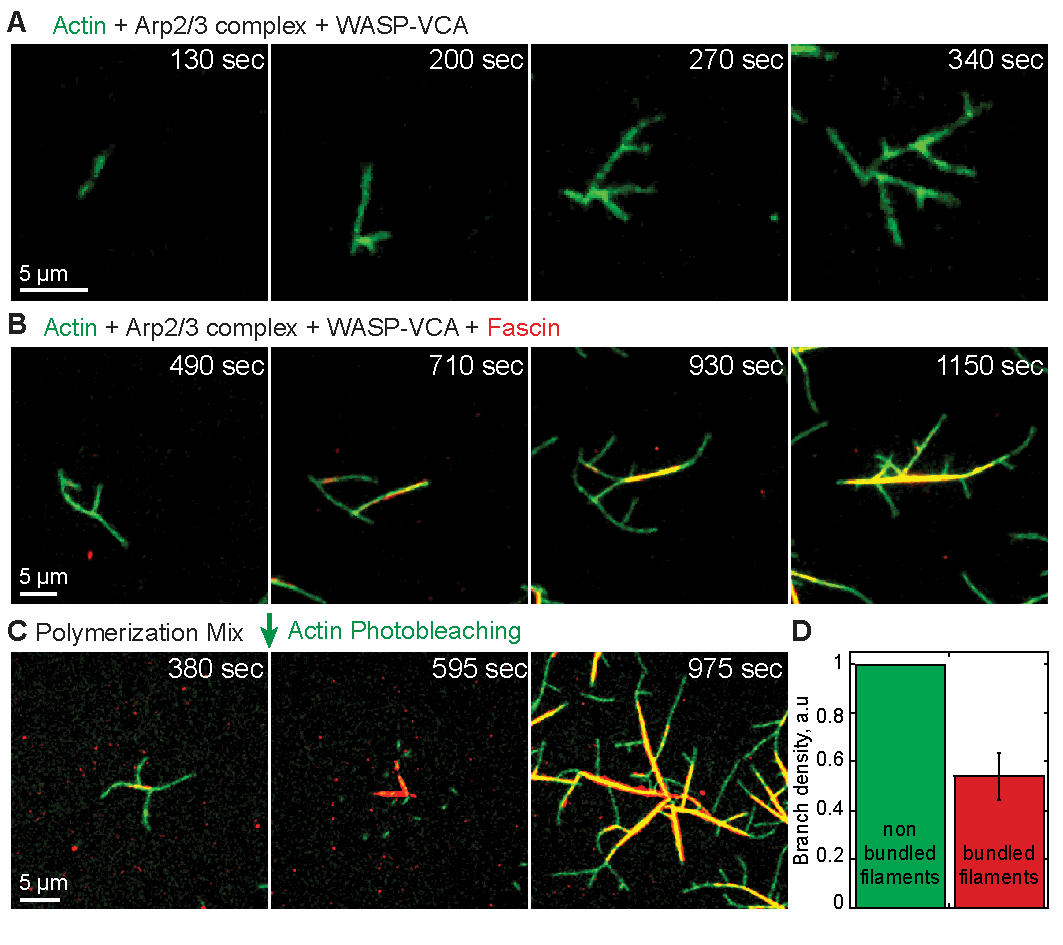
\includegraphics[width=\textwidth]{img/ch03/Thesis_branching.pdf}
\caption[Fascin reduces Arp2/3 complex-mediated branch density]{\textbf{Fascin reduces Arp2/3 complex-mediated branch density} (A) Arp2/3 complex-mediated actin polymerization. Conditions: 1.5 $\mu$M Oregon green-actin + 93 nM Arp2/3 complex + 300 nM WASP-VCA.
(B - C) Arp2/3 complex-mediated actin polymerization in absence (A) or presence (B and C) of fascin visualized by TIRFM. (C) Actin fluorescence is photobleached at t = 380 sec. Conditions: 1.5 $\mu$M Oregon Green-actin + 50 nM Arp2/3 complex + 100 nM WASP-VCA + 500 nM TMR-fascin. (D) Branch density from individual actin filaments and bundled filaments. Error bar, SE. n = 3. \textbf{Figure modified from Suarez et al. in preparation.}}
\label{fig:fascin_branching}
\end{figure}

\subsection{Fascin and \texorpdfstring{$\alpha$}{alpha}-actinin sort to distinct domains}
Fascin and $\alpha$-actinin sort to different domains \textit{in vitro}. The two bundling proteins fascin and $\alpha$-actinin have very different structures (Figure \ref{fig:em_fascin_aact}A). Fascin is a small globular protein containing  four $\beta$-trefoil domains. In contrast, $\alpha$-actinin forms a long homodimer using four spectrin repeats and binds to actin using CH domains. We originally observed fascin and $\alpha$-actinin sorting to distinct domains using TIRFM; however, we were interested in seeing the transition state between the bundling domains at a higher resolution. Therefore, we performed negative-stain electron microscopy (EM) to visualize pre-formed actin filaments mixed with either fascin or $\alpha$-actinin alone or both bundling proteins (Figure \ref{fig:em_fascin_aact}B). With fascin alone we see narrowly spaced filaments with an interfilament distance of \mytilde8 nm (Figure \ref{fig:em_fascin_aact}D) and a transverse repeat of \mytilde35 nm, which corresponds with one turn of F-actin. $\alpha$-actinin bundles alone have wider spaced filaments (\mytilde32 nm) with a similar transverse repeat of \mytilde35 nm (Figure \ref{fig:em_fascin_aact}C-D). As expected, when both bundlers are mixed together each domain has the characteristics of the respective bundler. The fascin domain is narrow (8 nm) and the $\alpha$-actinin domain is widely spaced (32 nm) (Figure \ref{fig:em_fascin_aact}C-D). We also observe a transition area (142$\pm$53 nm) between the two domains where the filaments become more widely spaced as you transition from a fascin domain to an $\alpha$-actinin domain (Figure \ref{fig:em_fascin_aact}B). 

\begin{figure}
\centering
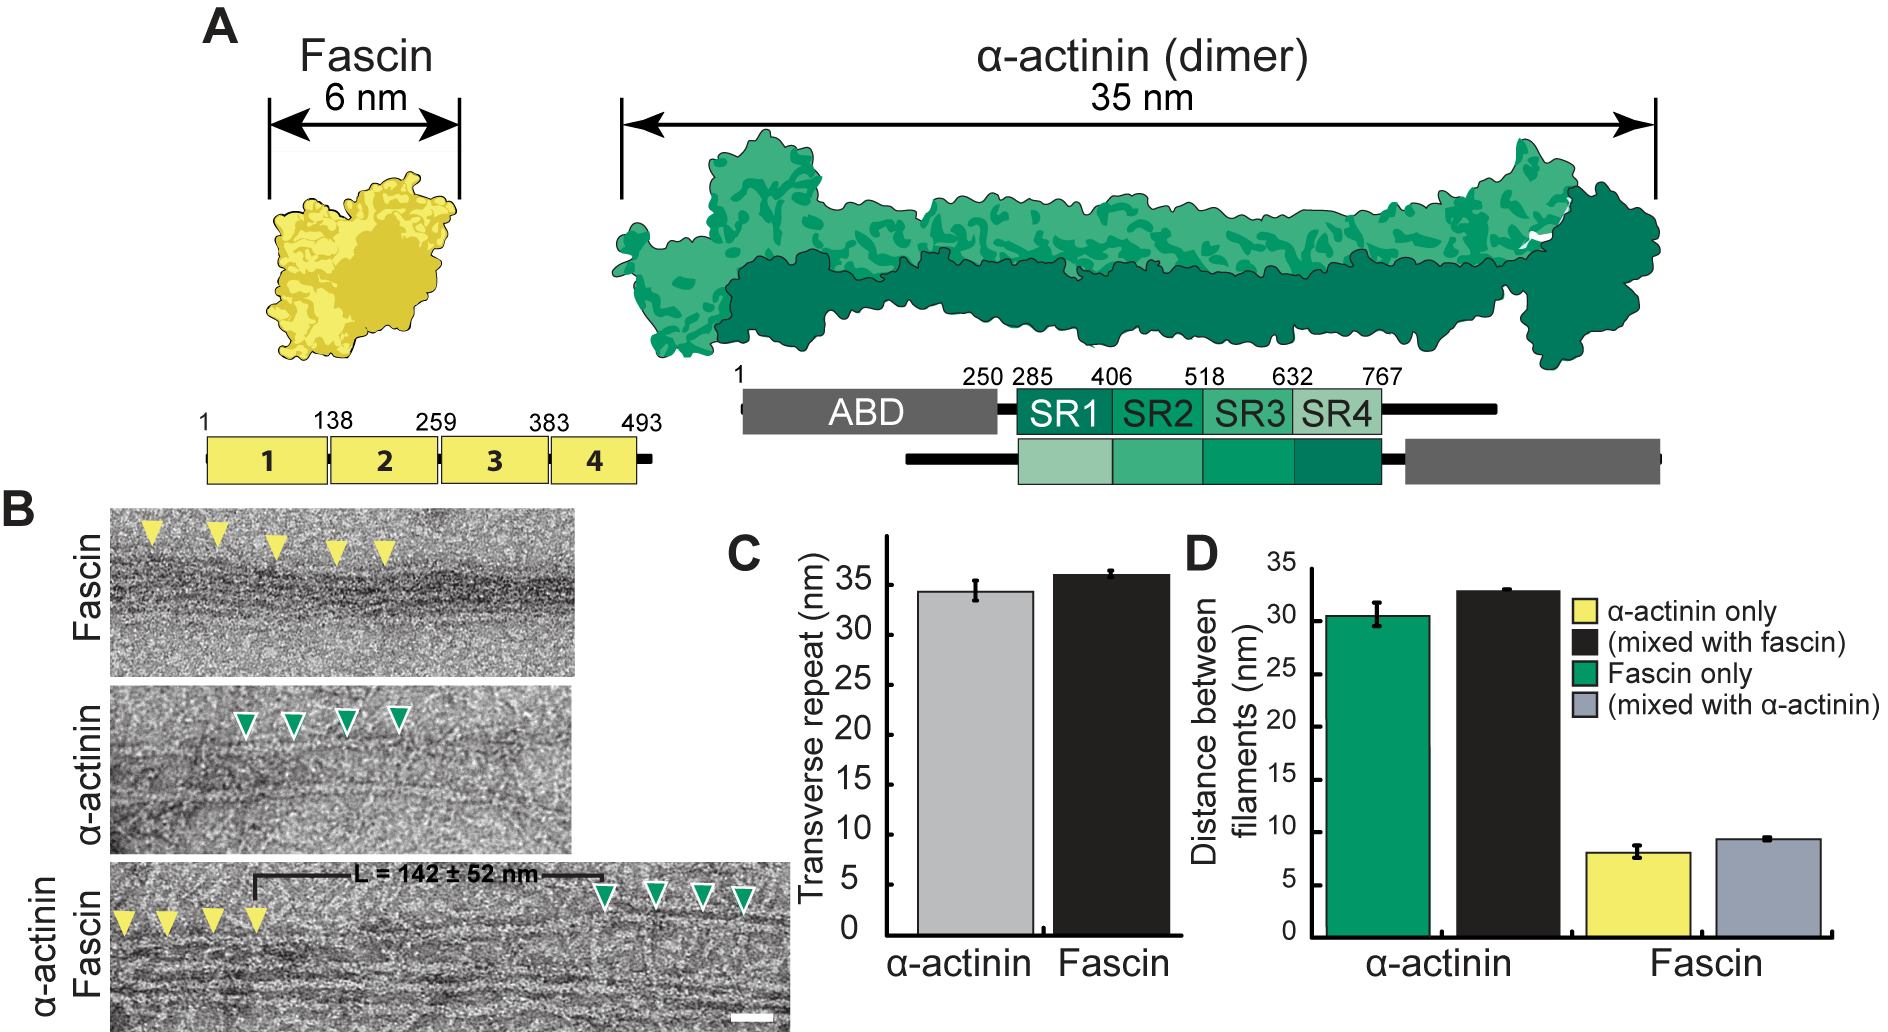
\includegraphics[width=14cm]{img/ch03/Thesis_EM_fig.png}
\caption[Fascin and \texorpdfstring{$\alpha$}{alpha}-actinin sort to different domains with different interfilament spacing.]{\textbf{Fascin and $\alpha$-actinin sort to different domains with different interfilament spacing.} (A) Structural fold (top) and domain organizations (bottom) showing the four $\beta$-trefoil domains of fascin (PDB 3P53; \citep{jansen_mechanism_2011}) (left) and an $\alpha$-actinin dimer (PDB 1SJJ; {liu a 3D}) (right). ABD, Actin-binding domain; SR, spectrin repeat. (F–H) Electron microscopy (EM) of F-actin bundles negatively stained with uranyl acetate, which were formed from 1.5 $\mu$M actin.(F) Micrographs of bundles with 1 $\mu$M fascin (top), 800 nM $\alpha$-actinin (middle) or both (1 $\mu$M $\alpha$-actinin 0.25 $\mu$M fascin (bottom). Yellow and green arrowheads indicate fascin and $\alpha$-actinin molecules. L is length of transition zone. Scale bar = 30 nm. (G) Distance of transverse repeat in fascin and $\alpha$-actinin bundles. Error bars indicate SEM; $n\geq10$ bundles. (H) Distance between filaments in a fascin and $\alpha$-actinin bundles. Error bars indicate SEM; $n\geq8$ bundles. Figure adapted from \citep{winkelman_fascin-_2016}. \textbf{EM in collaboration with Cristian Suarez. Figure modified from \citep{winkelman_fascin-_2016}}}
\label{fig:em_fascin_aact}
\end{figure}

%check fold values
\subsection{Tropomyosin effects \texorpdfstring{$\alpha$}{a}-actinin dynamics}
We have observed that S. Pombe tropomyosin, Cdc8, allows $\alpha$-actinin, Ain1, to form more stable bundles \citep{christensen_competition_2017}?. Fimbrin, Fim1 can compete either tropomyosin and $\alpha$-actinin off of F-actin. However, We recently discovered that, together, $\alpha$-actinin and tropomyosin are able to outcompete fimbrin. However, together both of these proteins are able to withstand fimbrin. To understand the mechansims of how this cooperation occurs we measured the dynamics of single-molecules of $\alpha$-actinin in the presence and absence of tropomyosin. We found that in the presence of tropomyosin, $\alpha$-actinin is more dynamic. There are 3-fold more binding events on F-actin when tropomyosin is present. Therefore, tropomyosin is enhancing $\alpha$-actinin's association with F-actin and subsequently improving $\alpha$-actinin's bundling properties. 


\begin{figure}
\centering
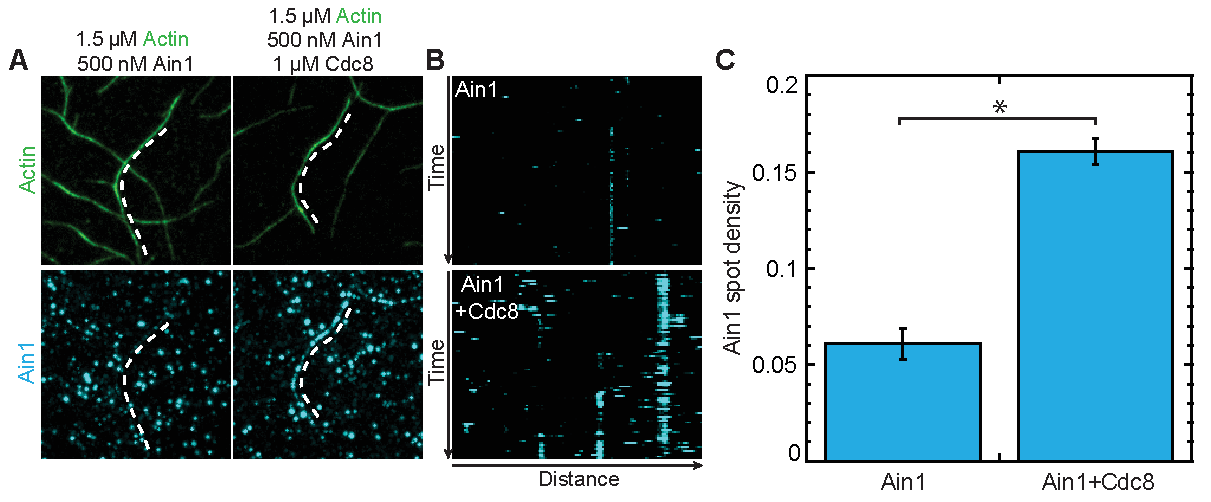
\includegraphics[width=\textwidth]{img/ch03/Thesis_aact_dynamics.pdf}
\caption[Tropomyosin increases \texorpdfstring{$\alpha$}{alpha}-actinin dynamics.]{\textbf{Tropomyosin increases $\alpha$-actinin dynamics.} TIRFM visualization of 1.5 $\mu$M Mg-ATP-actin (10\% Alexa 488-actin) with 500 nM 0.5\% TMR labeled $\alpha$-actinin Ain1, and 1 $\mu$M unlabeled tropomyosin Cdc8. (A) Time-lapse micrographs of actin or sparsely labeled $\alpha$-actinin. Dotted line denotes bundle in both channels. Scale bar, (B) Kymograph of actin bundle length (scale bar, ) over time (time bar, ). (C) Spot density of $\alpha$-actinin \textbf{Analysis in collaboration with Cristian Suarez. Figure modified from Christensen et al. in preparation.}}
\label{fig:tropo_aact}
\end{figure}


\section{Materials and Methods}\label{bundlers-matmeth}

% fix this specifically for this experiment
\subsection{Visualizing Arp2/3 complex branching in TIRFM}
TIRFM images were collected at 250ms-1s intervals with a cellTIRF 4Line system (Olympus, Center Valley, PA) fitted to an Olympus IX-71 microscope with through-the-objective TIRF illumination and an iXon EMCCD camera (Andor Technology, Belfast, UK). Mg-ATP-actin (15\% Oregon Green or Alexa 488 labeled) was mixed with polymerization TIRF buffer [10 mM imidazole (pH 7.0), 50 mM KCl, 1 mM MgCl\textsubscript{2}, 1 mM EGTA, 50 mM DTT, 0.2 mM ATP, 50 $\mu$M CaCl\textsubscript{2}, 15 mM glucose, 20 $\mu$g/mL catalase, 100 $\mu$g/mL glucose oxidase, and 0.5\% (400 centipoise) methylcellulose] to induce F-actin assembly and any additional actin binding proteins. This mixture was transferred to a flow cell for imaging at room temperature. For two color TIRFM, we cyclically imaged labeled actin (1 frame, 488 nm excitation for 50ms) and SNAP(549)-Ena/VASP (1 frame, 561 nm excitation for 50ms) \citep{winkelman_ena/vasp_2014}.
% need lab notebook for this
\subsection{Measuring Arp2/3 complex branch density}
Branch density...

\subsection{Visualizing F-actin bundles with negative-stain electron microscopy}
Actin (1.5 $\mu$M) was polymerized with either 250–500 nM $\alpha$-actinin, 1–2 $\mu$M fascin, or both bundling proteins for 30 min. This solution was then applied to formvar- and carbon-coated 400 mesh copper grids for 1 min, washed, and negatively stained with 1\% (w/v) uranyl acetate for 1 min, blotted, and dried. Visualization of the bundles using transmission electron microscopy was performed on an FEI Tecnai G2 Spirit microscope at 120 kV. Images were captured on a Gatan 2k $\times$ 2k CCD camera. Bundle parameters were measured using ImageJ.

\subsection{\texorpdfstring{$\alpha$}{a}-actinin Dynamics in TIRFM}
TIRFM images were collected with a cellTIRF 4Line system (Olympus) fitted to an Olympus IX-71 microscope with through-the-objective TIRF illumination and an iXon EMCCD camera (Andor Technology, Belfast, UK). 1.5 $\mu$M Mg-ATP-actin (10\% Alexa 488 labeled) was mixed with polymerization TIRF buffer [10 mM imidazole (pH 7.0), 50 mM KCl, 1 mM MgCl\textsubscript{2}, 1 mM EGTA, 50 mM DTT, 0.2 mM ATP, 50 $\mu$M CaCl\textsubscript{2}, 15 mM glucose, 20 $\mu$g/mL catalase, 100 $\mu$g/mL glucose oxidase, and 0.5\% (400 centipoise) methylcellulose] to induce F-actin assembly, 0.5 $\mu$M 0.5\% TMR labeled $\alpha$-actinin, and 1 $\mu$M unlabeled tropomyosin. This mixture was transferred to a flow cell for imaging at room temperature. Once the actin had polymerized and formed bundles we imaged once in the 488 channel to visualize the labeled actin (1 frame, 488 nm excitation for 50ms) and then continuously imaged in the 561 channel to visualize the sparsely labeled $\alpha$-actinin (100 frames, 561 nm excitation for 50 ms, \mytilde110 ms interval).
To measure $\alpha$-actinin spot density, we constructed kymographs of bundles for each experiment using ImageJ. $\alpha$-actinin spots were detected in the kymograph as spots at least 4 pixels wide with fluorescence more than 1.25-fold above background fluorescence. We normalized the spot density to the length of actin filaments present in the bundle. At this end, we measure bundles length, then multiply the value by the actin fluorescence ratio between a bundle and single filament. $\alpha$-actinin spot density was determined following the formula: 
\[\rho = \frac{(n/(L\times r))}{t}\]
Where $n$ is the number of $\alpha$-actinin spots detected, $L$ the length of the bundle in $\mu$m, $r$ the actin fluorescence ratio, and $t$ the time of measurement in seconds.




% Chapter 04
\chapter{Pathogenic bacteria can affect the endogenous actin cytoskeleton}\label{ch:vibrio}

\section[Abstract]{Abstract\footnotemark}
\textit{Vibrio cholera} has multiple ways to interfere with a host cell’s actin cytoskeletal system. I collaborated on two projects to better understand the different pathways that gram-negative \textit{Vibrio} bacteria can commandeer the actin cytoskeleton. The actin cytoskeleton is an ideal target for pathogenic bacteria for diverse reasons and pathogens target the actin cytoskeleton using different methods. The actin cytoskeleton can be used to prevent or induce the pathogen's phagocytosis as well as facilitate their movement into, around, and out of host cells \citep{liverman_arp2/3-independent_2007}. 

The first collaboration with Tom Burke in the Kovar lab focused on the mechanism of actin nucleators, VopL and VopF. These \textit{Vibrio} nucleators assemble actin into unproductive filament within host cells. There were controversial mechanisms proposed for how these proteins were able to nucleate actin filaments and we presented a solution to this controversy, showing that in the presence of physiological conditions that VopL and VopF nucleate and bind to the pointed ends of F-actin. In the second collaboration with the Kudryashov lab at The Ohio State University, I used single-molecule TIRFM to visualize the effect of ACD toxin-formed actin oligomers on Ena/VASP. The Kudryashov lab had previously found that these toxic oligomers affect formin elongation \citep{heisler_acd_2015}, and in this study we expanded to other endogenous actin assembly factors. 

Overall these two works contribute to understanding mechanisms for how pathogenic bacteria can interfere with a host's actin cytoskeleton. Understanding how \textit{Vibrio} bacteria can hijack the endogenous actin system allows us to better fight the disease-causing bacteria. I have presented below the data from the collaborations that I had a role collecting and analyzing and focus on the aspects of the studies that are relevant to my contribution. 

\footnotetext{Citations for chapter: [1] Thomas A. Burke, Alyssa J. Harker, Roberto Dominguez, and David R. Kovar. The bacterial virulence factors VopL and VopF nucleate actin from the pointed end. \textit{The Journal of Cell Biology}, March 2017. [2] Elena Kudryashova, David B. Heisler, Blake Williams, Alyssa J. Harker, Kyle Shafer, Margot E. Quinlan, David R. Kovar, Dimitrios Vavylonis, and Dmitri S. Kudryashov. Actin Cross-Linking Toxin Is a Universal Inhibitor of Tandem-Organized and Oliogmeric G-Actin Binding Proteins. \textit{Current biology}, 28{10}:1536-1547.e9, May 2018.}

\section{Introduction}\label{ch04-introduction}
Bacterial toxins can effectively compromise a host cell's functions with relatively few molecules, even leading to cell death. These toxins can target signaling cascades (ex. cGMP, adenylate cyclase) or inhibit other enzymes important for cellular processes such as protein synthesis \citep{henkel_toxins_2010}. As the actin cytoskeleton is important for many cellular processes, it is commonly targeted by bacterial toxins. The actin crosslinking domain (ACD) toxins of \textit{Vibrio} species and related bacterial genera are delivered to host cells by type 1 (MARTX toxin) \citep{sheahan_identification_2004} or type VI (VgrG1 toxin) secretion systems \citep{pukatzki_type_2007}. ACD catalyzes formation of actin oligomers through covalent crosslinking of Lys50 in subdomain 2 of an actin monomer with Glu270 in subdomain 3 of another actin monomer by an amide bond \citep{kudryashov_connecting_2008,kudryashova_glutamyl_2012}. This results in an oligomer that is not suitable for further actin polymerization because the two monomers are oriented similar to actin subunits along the short pitch of an actin filament, except that subdomain 2 has a major twist, disrupting the normal interface for further monomer binding \citep{kudryashov_connecting_2008}. 

Surprisingly, though there is a high concentration of actin, only a few ACD molecules are secreted into the host cell. Using \textit{in vitro} determined rates of ACD activity, it would take more than 6 months to covalently crosslink half of all the cytoplasmic actin with a single ACD molecule. This is beyond the timescale for \textit{in vivo} measurements of monolayer disruption \citep{kudryashova_glutamyl_2012, heisler_acd_2015}. In a previous collaboration with the Kudryashov lab, we found that ACD is effective not by sequestering monomers as previously thought but by using actin oligomers to target formins \citep{heisler_acd_2015}. We found that ACD formed toxic actin oligomers that blocked formin-mediated actin polymerization and nucleation. However, the mechanism of how these ACD-formed oligomers block formin activity remains unclear. 

Another way that bacteria target the actin cytoskeleton is through type III secretion factors VopF (\textit{Vibrio cholerae}) or VopL (\textit{Vibrio parahaemolyticus}) (VopL/F) \citep{tam_type_2007,liverman_arp2/3-independent_2007}. VopL/F contain three tandem WASP homology 2 (WH2) motifs followed by a VopL/F C-terminal Domain (VCD) that facilitates dimerization (Figure \ref{fig:vop}A). This places VopL/F into the class of WH2 nucleators such as cordon-bleu and Spire \citep{qualmann_new_2009}. The WH2 domain is able to bind to actin monomers in the target-binding cleft between actin subdomains 1 and 3 to facilitate actin filament nucleation \citep{namgoong_mechanism_2011}. The mechanisms of the WH2 nucleators are not as well studied as other nucleators, Arp2/3 complex and formins. 

VopL/F have a 32\% sequence identity and 72\% sequence similarity and contain the same domain organization, though two competing mechanistic models have been previously proposed. Two groups proposed that VopL nucleates actin filaments from the pointed end and then remains associated with the new filament for only a short time \citep{namgoong_mechanism_2011, yu_mechanism_2011} while a third group proposed that VopF binds to the barbed end of growing F-actin and can also sever filaments \citep{pernier_dimeric_2013}. In support for the pointed end nucleation model, the crystal structure of VopL in complex with actin was solved and showed that the VCD dimer binds to three actin monomers in an arrangement that is similar to F-actin and allows each actin subunit to bind to a WH2 motif \citep{zahm_bacterial_2013}. We set out to clear up this controversy by using single-molecule TIRFM to visualize VopL/F binding to filaments \citep{burke_bacterial_2017}. 

\section{Results}\label{ch04-results}

\subsection{Ena/VASP is inhibited by actin crosslinking toxins}\label{ena-acd-oligomers}
Our previous study showed that formin mediated elongation of F-actin is blocked by ACD oligomers in a concentration dependent manner \citep{heisler_acd_2015}. We measured the IC\textsubscript{50} of ACD oligomer inhibition of mDia1 to be 1.2 $\pm$ 0.6 nM. To further understand the mechanism of how these ACD oligomers affect actin assembly factors we measured their effect on Ena/VASP. We used two-color single-molecule TIRFM to directly visualize the assembly of 1.5 $\mu$M Mg-ATP-actin monomers (15\% Oregon green-labeled) with 15 pM fluorescently labeled SNAP(549)-Ena$\Delta$L (referred to as Ena), 3 $\mu$M Chickadee (fly profilin), and an increasing concentration of ACD oligomers (Figure \ref{fig:ena-oligomers}A-C). We measured the activity of Ena on barbed ends of actin filaments and recorded the barbed end elongation rate while Ena was bound. We found that Ena is affected by the ACD oligomers and will cap filaments, blocking growth (Figure \ref{fig:ena-oligomers}. We calculated the percentage of capped filaments over a range of ACD oligomers and found that with increasing ACD oligomers, Ena behaved more often as a capping protein than a elongation factor. We also observed that the run length of Ena was much longer when growth of the filament was stopped than while the filament was elongating. This suggests that the oligomers affect Ena's mechanism in a way to reduce the chance of its dissociation from the barbed end. 

\begin{figure}
\centering
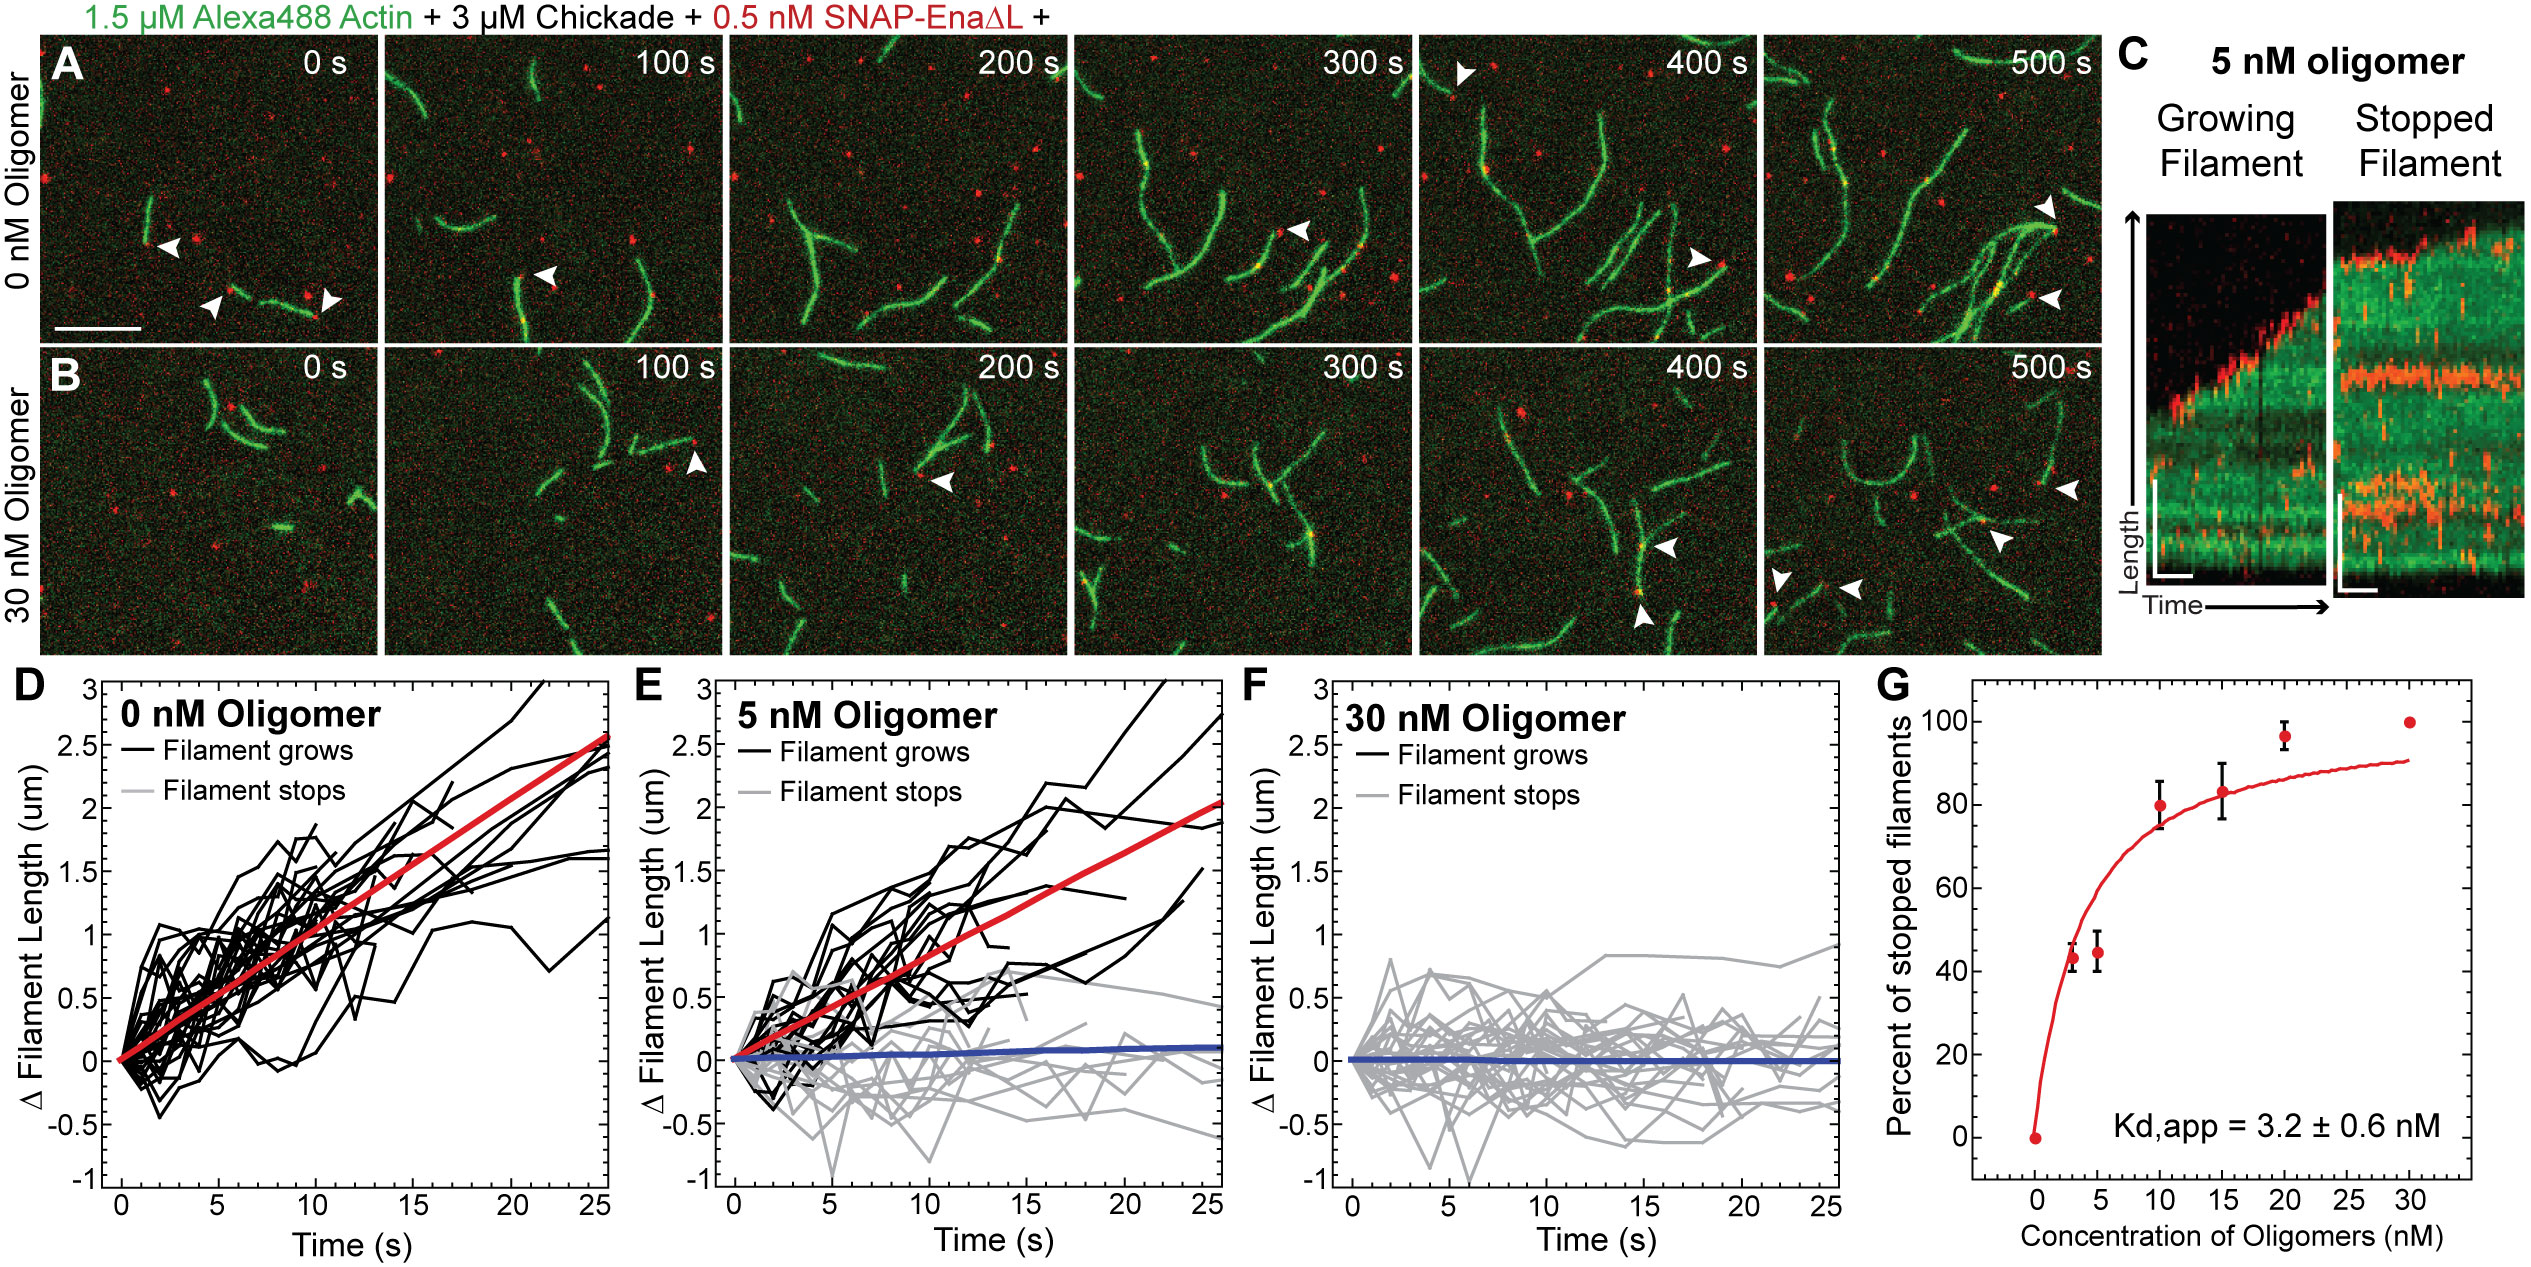
\includegraphics[width=\textwidth]{img/ch04/Oligomer_Ena_Figure.jpg}
\caption[Actin oligomers stop Ena-mediated processive filament elongation.]{\textbf{Actin oligomers stop Ena-mediated processive filament elongation.} Two color TIRFM timelapse of 1.5 $\mu$M Alexa-488 actin (green) and 0.5 nM SNAP-Ena$\Delta$L (red) in the presence of 3 $\mu$M Chickadee (fly profilin) and (A) no actin oligomers or (B) 30 nM actin oligomers. Arrows indicate Ena bound barbed ends. Scale bar, 10 $\mu$m. Kymographs of a (C) growing Ena bound filament (left) and a stopped Ena bound filament (right). Scale bar, 4 $\mu$m and 10 s. Filament elongation traces of Ena bound filaments with (D) 0 nM Oligomers, (E) 5 nM Oligomers, and (F) 30 nM Oligomers. Red fit lines show average growth rates of Ena bound growing filaments and blue fit lines show average growth rates of Ena bound stopped filaments. (G) Kd,app determined by TIRFM by percent of stopped Ena bound filaments over a range of actin oligomers. \textbf{Figure modified from \citep{kudryashova_actin_2018}}.}
\label{fig:ena-oligomers}
\end{figure}

\subsection{VopL and VopF assemble endogenous actin}\label{vops}
To investigate the molecular mechanism of VopL/F actin nucleation we wanted to directly visualize labeled VopL/F using single-molecule TIRFM. We assembled 1.5 $\mu$M Mg-ATP-actin (15\% Oregon green-labeled) in the presence of 0.2 nM 549-SNAP-VopL/F to measure the elongation rate of actin filaments and the lifetime of VopL/F bound (Figure \ref{fig:vop}E-F). We observed that in the presence of growing filaments, VopL/F nucleates actin polymerization and binds to one end of actin filament as the filament continues to elongate. Barbed end associating proteins are known to typically affect the elongation rate of F-actin while they are bound (i.e. formins \citep{kovar_molecular_2006}). Therefore, we measured the elongation rate of VopL/F bound filaments (\mytilde13.0 sub/s) and found no difference in elongation rate compared to control filaments (Figure \ref{fig:vop}B-C). We measured the residence time of VopL and VopF to understand its dynamics on ends of filaments. Kaplan-Meier plots were used to calculate the average lifetime of bound VopL/F after nucleating the actin filament. However, since there is dead time required to flow in the reaction (\mytilde20 s) and for the time required for nascent filaments to grow long enough to be seen due to the resolution of the microscope (\mytilde0.5 $\mu$m), we calculated two different residence times. The first residence time ($\tau$\textsubscript{Obs}) is from the observed timepoint where an actin filament and VopL/F protein are first visualized with TIRFM until the VopL/F protein dissociates from the filament. The second residence time ($\tau$\textsubscript{Calc}) takes into account how long before the filament is able to be visualized due to the flow delay and resolution of TIRFM. Overall we observe that both VopL and VopF bind to the end of filaments for a similar amount of time using either the observed residence time (VopL\textsubscript{Obs} $\tau$ = 35 s, VopF\textsubscript{Obs} $\tau$ = 27 s) or the calculated residence time (VopL\textsubscript{Calc} $\tau$ = 104 s, VopF\textsubscript{Calc} $\tau$ = 110 s). 

By creating kymographs of the filaments over time we see that VopL/F binds to the pointed, slow-growing end. Another way to identify the pointed end in TIRFM is by using the fluorescence intensity along a filament. Due to photobleaching, the pointed end, which has been assembled for a longer amount of time, is dimmer than the newly assembled actin at the barbed end (Figure \ref{fig:vop}F). We see using linescans that VopL/F associates with this dimmer, pointed end (Figure \ref{fig:vop}H-I). In contrast, formin mDia2, a known barbed end-binding protein, binds to the brighter barbed end (Figure \ref{fig:vop}J). Therefore, VopL/F nucleates filaments and then binds to the dimmer, pointed end of F-actin for \mytilde110 s before dissociating from the filament.

\begin{figure}
\centering
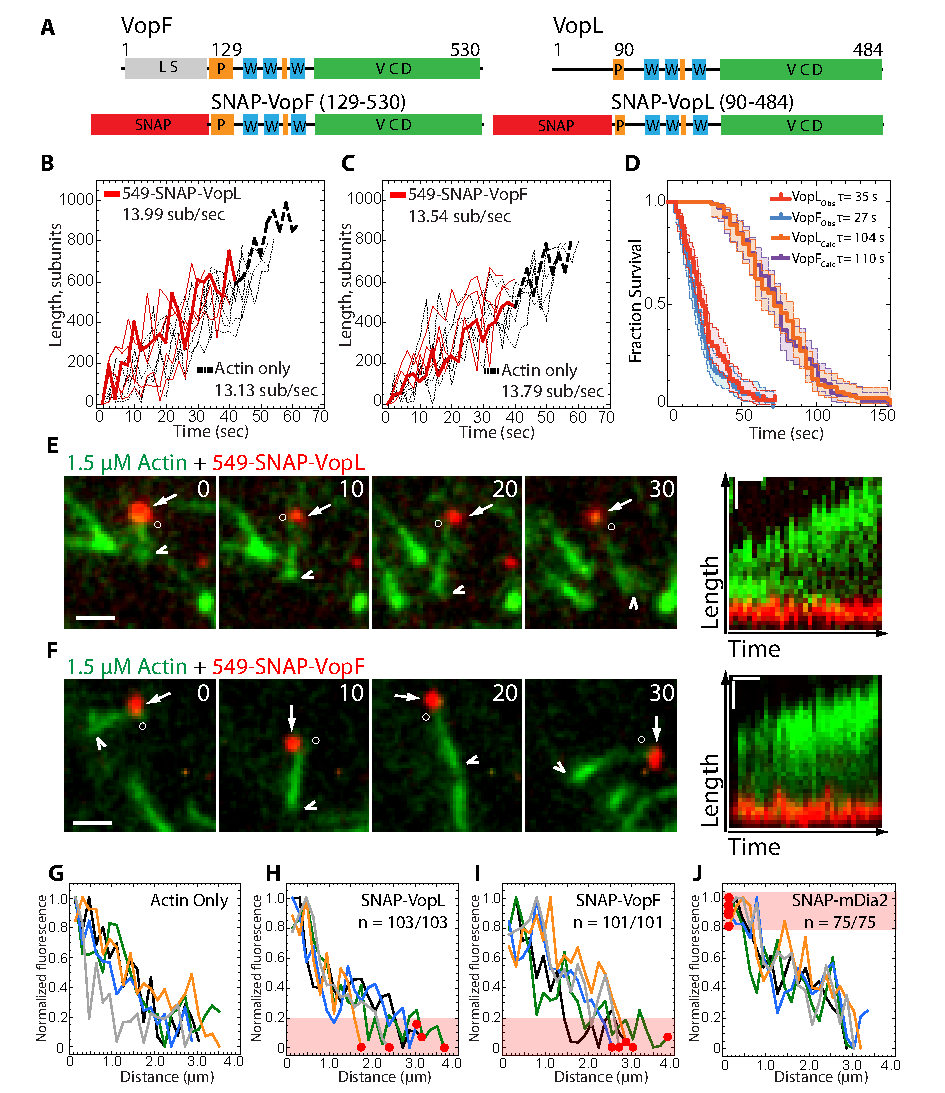
\includegraphics[width=\textwidth]{img/ch04/Thesis_Vop.pdf}
\caption[ VopL/F nucleate and then remain briefly associated with the pointed end of an actin filament.]{\textbf{ VopL/F nucleate and then remain briefly associated with the pointed end of an actin filament.} (A) Top, domain organization of VopL/F. Orange, proline-rich region (P); blue, WH2 domain (W); green, VCD dimerization domain. Bottom, VopL/F constructs used in this study with SNAP tag (red) for labeling.}
\label{fig:vop}
\end{figure}

% Continues caption on next page. Requires package ccaption.
\begin{figure}[!htb]
  \contcaption{(continued) (B–J) Slow acquisition (every 2 s, B–D) and rapid acquisition (every second, E–J) two-color TIRFM of the assembly of 1.5 $\mu$M Mg-ATP-actin (15\% Oregon green actin) with 0.2 nM 549(red)-SNAP-VopL/F. (B and C) Length of individual control (dashed black), 549-SNAP-VopL–associated (B, solid red), or 549-SNAP-VopF-associated (C, solid red) filaments over time ($n \geq 20$). (D) Kaplan–Meier curves representing the mean residence time of 549-SNAP-VopL/F on actin filaments observed (VopL\textsubscript{Obs}, VopF\textsubscript{Obs}) or assumed to have been associated because of nucleation (VopL\textsubscript{Calc}, VopF\textsubscript{Calc}). Error bars indicate 95\% CI; $n \geq 90$ events. (E and F, left) Merged timelapse micrographs (in seconds) of individual filaments. White arrowheads and open circles indicate bright and dim filament ends. White arrows indicate 549-SNAP-VopL/F. Scale Bars, 2 $\mu$m. (E and F, right) Merged kymographs of filament length (y axis; bar, 1 $\mu$m) over time (x axis; bar, 10 s) of the corresponding filaments. (G–J) Linescans of the normalized fluorescence intensity of individual actin filaments measured from their bright to dim (bleached) ends. Red dots indicate position of 549-SNAP-VopL/F or 549-SNAP-mDia2 on the filament traces, and shaded red regions indicate where 100\% of VopL/F or mDia2 are bound to the filaments (n $\geq$ 75). \textbf{TIRFM, elongation rate, and linescan analysis completed by Tom Burke. Figure modified from \citep{burke_bacterial_2017}.}}
\end{figure}

\section{Materials and Methods}\label{mat-meth-vib}
\subsection{ACD oligomer and Ena TIRFM}\label{oligo-mm-tirf}
TIRFM images were collected at 1 s intervals with a cellTIRF 4Line system (Olympus, Center Valley, PA) fitted to an Olympus IX-71 microscope with through-the-objective TIRF illumination and an iXon EMCCD camera (Andor Technology, Belfast, UK). Mg-ATP-actin (15\% Alexa 488 labeled) was mixed with polymerization TIRF buffer [10 mM imidazole (pH 7.0), 50 mM KCl, 1 mM MgCl\textsubscript{2}, 1 mM EGTA, 50 mM DTT, 0.2 mM ATP, 50 $\mu$M CaCl\textsubscript{2}, 15 mM glucose, 20 $\mu$g/mL catalase, 100 $\mu$g/mL glucose oxidase, and 0.5\% (400 centipoise) methylcellulose] to induce F-actin assembly and 0.5 nM SNAP(549)-Ena$\Delta$L, 3 $\mu$M chickadee, and the noted concentration of ACD oligomers. This mixture was transferred to a flow cell for imaging at room temperature. For two color TIRFM, we cyclically imaged labeled actin (1 frame, 488 nm excitation for 50ms) and SNAP(549)-Ena$\Delta$L (1 frame, 561 nm excitation for 50ms) \citep{winkelman_ena/vasp_2014}. 

\subsection{Analysis of Ena/VASP elongation}
Barbed end elongation rates were calculated by measuring filament lengths over time with ImageJ software. Measurements of ten filaments with at least 6 length measurements at different time points from three different movies for each condidtion were made.  Multiple filament lengths were plotted over time and the distribution was fit with a linear equation using KaleidaGraph 4.5 (Synergy Software, Reading, PA). Filaments were counted as stopped if they had an elongation rate less than 5 sub/s and growing if the elongation rate was greater than 15 sub/s. The apparent Kd was calculated using the following quadratic equation, \[f(x) = \frac{(x + m1 + 1)-\sqrt{(x+m1+1)^2-4*x*1)}}{2}\] where m1 was set equal to 1, as the data was normalized from 0 to 1 \citep{pollard_guide_2010}.

\subsection{Analysis of VopL/F lifetime}
Residence times for 549-SNAP-VopL/F on nucleated actin filaments in spontaneous TIRFM assays were determined through back-calculation by measuring the length of actin filaments immediately before the 549-SNAP-VopL/F dissociated and converting that length into total actin subunits (1 $\mu$m = 375 subunits). The subunit length was divided by the mean elongation rate of the filaments. Barbed-end elongation rates were calculated by measuring filament lengths over time with ImageJ. Residence times for single 549-SNAP-VopL/F dimers were determined by fitting a Kaplan-Meier \citep{kaplan_nonparametric_1958} survival curve with a single exponential equation, $f(x) = x_{0} * exp^{(-x/\tau)}$ to calculate the average lifetime. Kaplan-Meier survival curves were used to account for processive runs that started before imaging began or ended after imaging terminated. Log rank statistical significance tests were done using Prism 7 (GraphPad Software, San Diego, CA). We reported two average lifetimes, one from observed time bound ($\tau$\textsubscript{Obs}) and other that is calculated accounting for the dead time required to flow the reaction into the chamber (\mytilde20 s) and for the filaments to reach an observable length (\mytilde0.5 $\mu$m) ($\tau$\textsubscript{Calc}).




% Chapter 05
% chapter 05
\chapter{Conclusions and Future Directions}\label{ch:conclusions}

\section{Ena/VASP mechanisms}\label{ena-mechanism-conclusions}
Understanding the mechanism of formins and their regulation by protein binding partners as well as outside forces has taken a step forward in the last few years. Though they mechanistic understanding of Ena/VASP lags behind that of formins great progress is being made in understanding how Ena/VASP can be processive and how it is functioning within cells. There has been initial insight in how these two processive polymerases work together within cells, but much more needs to be done to understand their collaboration and concurrent regulation. These processive polymerases are mechanistically interesting to compare and contrast to understand how different proteins maintain actin filament contact as well as how they are regulated within the cell. Understanding their individual functions as well as how they work together will give a clearer picture of what is happening at filopodia and the leading edge of the cell. 

\section{Ena/VASP and bundled actin filaments}\label{ena-bundles-conclusions}
Ena/VASP making filopodia:
mechanism with convergent elongation

Different actin networks, bundling protein can regulate
Fascin specific for filopodia

\section{Actin bundling proteins and their effect on other ABPs}\label{bundler-conclusions}

As we've seen with Ena, bundling proteins 
Effect on actin nucleation: fascin slower? Or not measured so shouldn't mention

\section{Pathogenic bacteria target the host actin cytoskeleton}\label{bacteria-conclusions}

\section{Concluding Remarks}\label{final-conclusions}

% Format a LaTeX bibliography
\makebibliography

% Figures and tables, if you decide to leave them to the end
%\input{figure}
%\input{table}

\end{document}


